\chapter{Determination of the Strong Coupling Constant}
\label{sec:Fits}
The inclusive jet production cross-section at hadron colliders mainly depends on the strong coupling constant \alps for a given centre-of-mass energy. Hence the measurements of the inclusive jet cross section and jet properties provide a direct probe to measure the strong coupling constant. The measurement of \alps has been already done by various experiments such as CMS~\cite{Chatrchyan:2013txa, Chatrchyan:2013haa, Khachatryan:2014waa, CMS:2014mna, Khachatryan:2016mlc}, ATLAS~\cite{ATLAS:2015yaa}, D0~\cite{Abazov:2009nc, Abazov:2012lua}, H1~\cite{Andreev:2014wwa, Andreev:2016tgi}, and ZEUS~\cite{Abramowicz:2012jz}. In this thesis, the measurements of differential inclusive 2-jet and 3-jet event cross sections as well as the cross section ratio \ratio, as a function of \httwo are used to extract the value of the strong coupling constant at  the  scale  of  the  Z boson mass \alpsmz. The differential inclusive jet production cross section upto at NLO is given by \cite{Affolder:2001hn}:

 \begin{equation}
 \frac{d\sigma}{d(\httwo)} = \alpha_S^2(\mur)\hat{X}^{(0)}(\muf,\httwo)\big[1~\plus \alpha_S(\mur)K1(\mur, \muf,\httwo)\big]
 \label{eqn:SigmaNLO}
 \end{equation}

 where $\frac{d\sigma}{d(\httwo)}$ is the differential inclusive jet production cross section as a function of \httwo, \mur and \muf are the renormalization and factorization scales set equal to \httwo, $\alpha_S^2(\mur)\hat{X}^{(0)}(\muf,\httwo)$ is the leading order (LO) contribution to the differential inclusive jet production cross section and $\alpha_S^3(\mur)\hat{X}^{(0)}(\muf,\httwo)K1(\mur, \muf,\httwo)$ is the next-to-leading order (NLO) contribution. Equation~\ref{eqn:SigmaNLO} shows how the inclusive jet production cross section varies with $\alpha_S(\mur)$. 
 
\section{Sensitivity of Measurements to \texorpdfstring{\alpsmz}{alpha-S(M(Z))}}
\label{sec:sensitivity}
 
For a fixed choice of \mur and \muf, different input values of \alpsmz to a PDF set will lead to different theory predictions of the differential cross section distribution. This will give an estimate of the sensitivity of the theory predictions to the varying input value of \alpsmz. A comparison of the measured spectrum with the theory predictions obtained using all \alpsmz inputs will give a hint of the input value of \alpsmz for which the theory distribution has the closest matching with data. In this section, the sensitivity of the inclusive differential jet event cross sections and cross section ratio, \ratio to varying input values of \alpsmz for different PDF sets is demonstrated by plotting the ratios of data over theory predictions with central value of \alpsmz.

Figures~\ref{fig:sensitivity_2},~\ref{fig:sensitivity_3} and~\ref{fig:sensitivity_double_ratio} present the ratio of data to the theory predictions, corrected for NP effects, for all variations in \alpsmz available for the PDF sets CT10, CT14, MSTW2008, MMHT2014 and NNPDF2.3 at NLO evolution order as specified in Table~\ref{tab:nlopdfsets}, for inclusive 2-jet, inclusive 3-jet events cross section and ratio \ratio respectively. The \alpsmz value is varied in the range 0.112-0.127, 0.111-123, 0.110-0.130, 0.108-0.128 and 0.114-0.124 in steps of 0.001 for the CT10, CT14, MSTW2008, MMHT2014 and NNPDF2.3PDF sets, respectively. The error bars correspond to the total experimental uncertainty derived as quadratic sum from all uncertainty sources. The theory predictions are also corrected for EW effects for inclusive 2-jet events cross section. A small slope increasing with \httwo is visible for most PDFs in both cross sections. This effect is largely cancelled in the cross section ratio. \ratio exhibits a flat behaviour with respect to the predictions for all five PDF sets in the whole range of \httwo up to 1680 GeV. Therefore, these data can be used to determine the strong coupling constant, although only up to 1 TeV for the cross sections as long as electroweak corrections are not taken into account.

Moreover, the different sensitivity to \alpsmz caused by the leading power in \alps in the expansion of the 2-jet inclusive ($\propto\alps^2$) and the 3-jet inclusive cross section ($\propto\alps^3$), and their ratio ($\propto\alps^1$) is clearly visible from the spread between the calculations for the smallest and largest value of \alpsmz within the same PDF set when passing through Figures~\ref{fig:sensitivity_2}--\ref{fig:sensitivity_double_ratio}.  This also demonstrates the potential of ratios $R_{mn}$ with $m$-$n$ \gr 1.

\begin{figure}[!htbp]
 \begin{center}
 \hspace*{-5mm}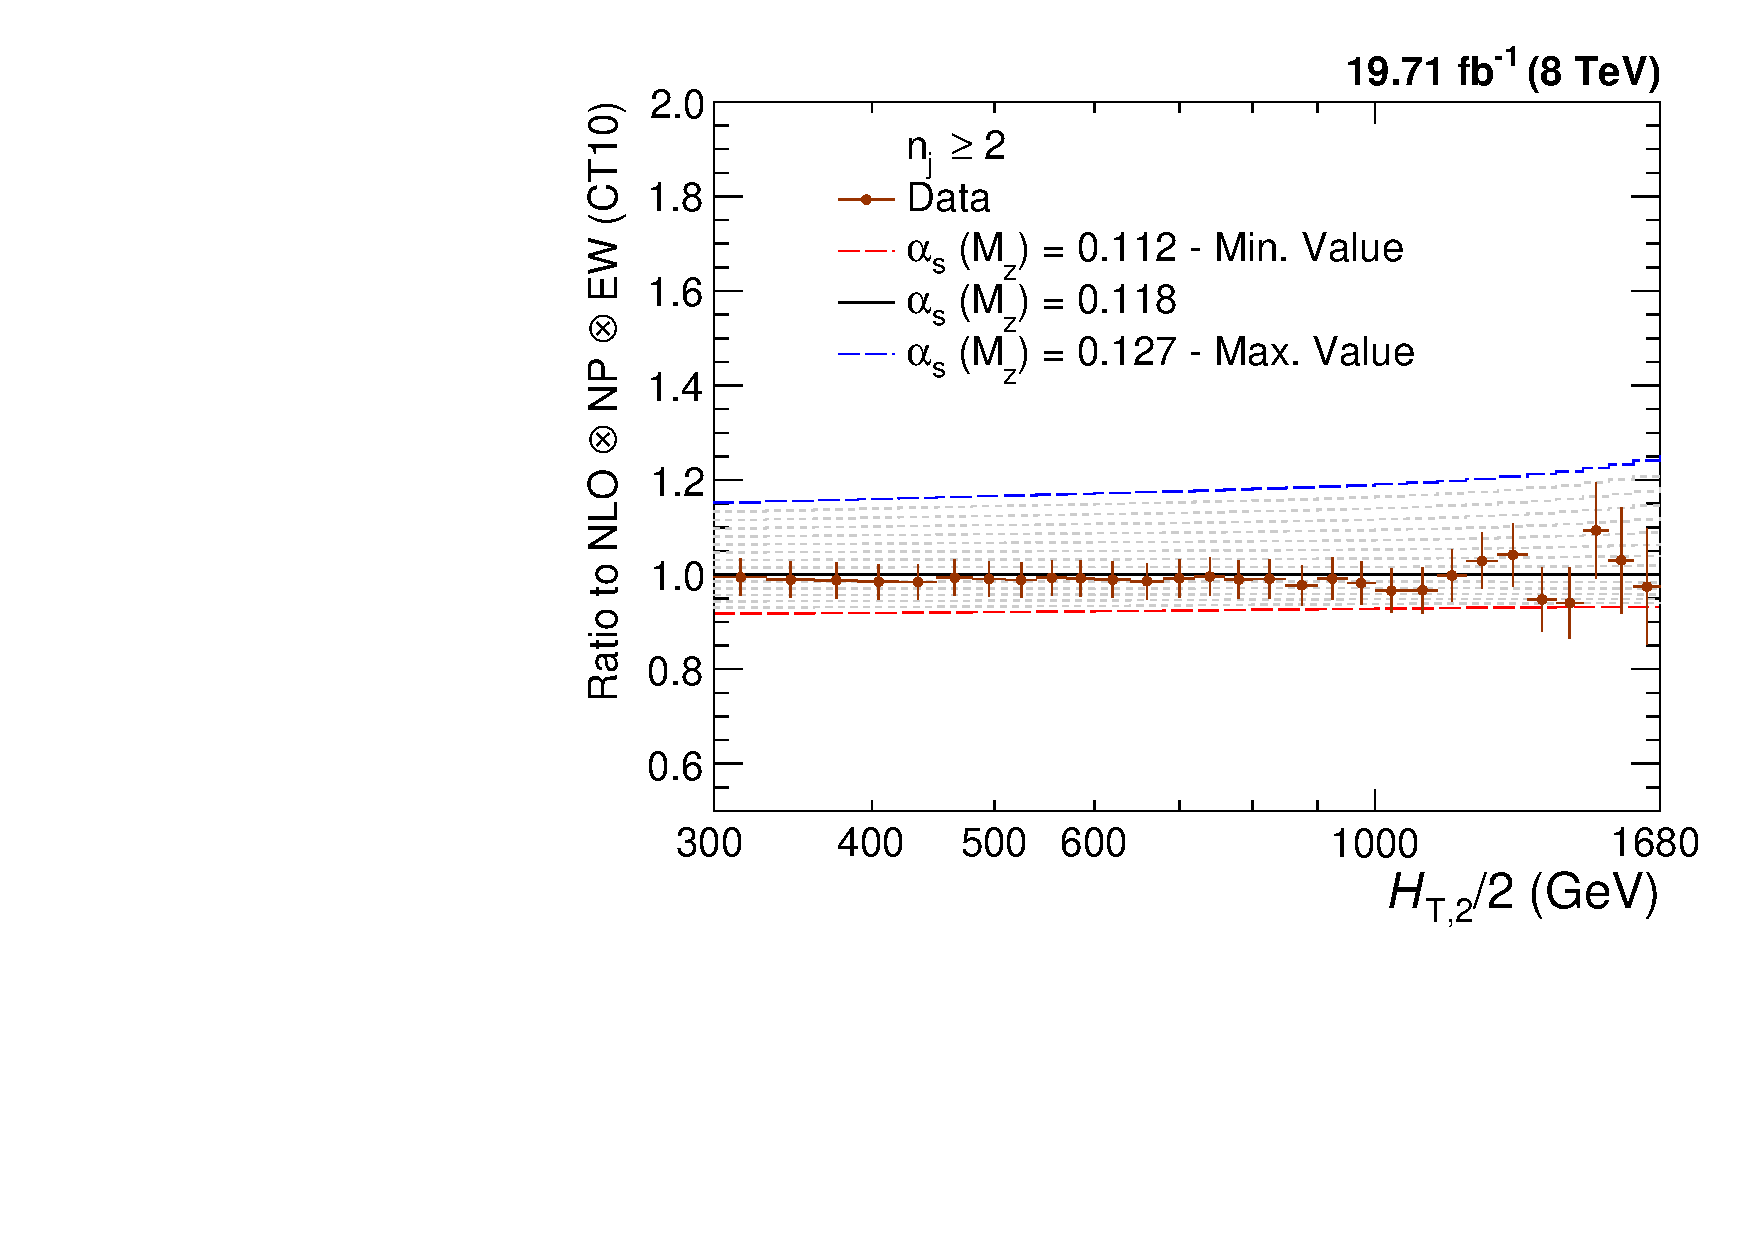
\includegraphics[width=0.51\textwidth]{Plots_HT_2_150/Sensitivity_2_ratio_NLO_CT10_EW.pdf}%
 ~~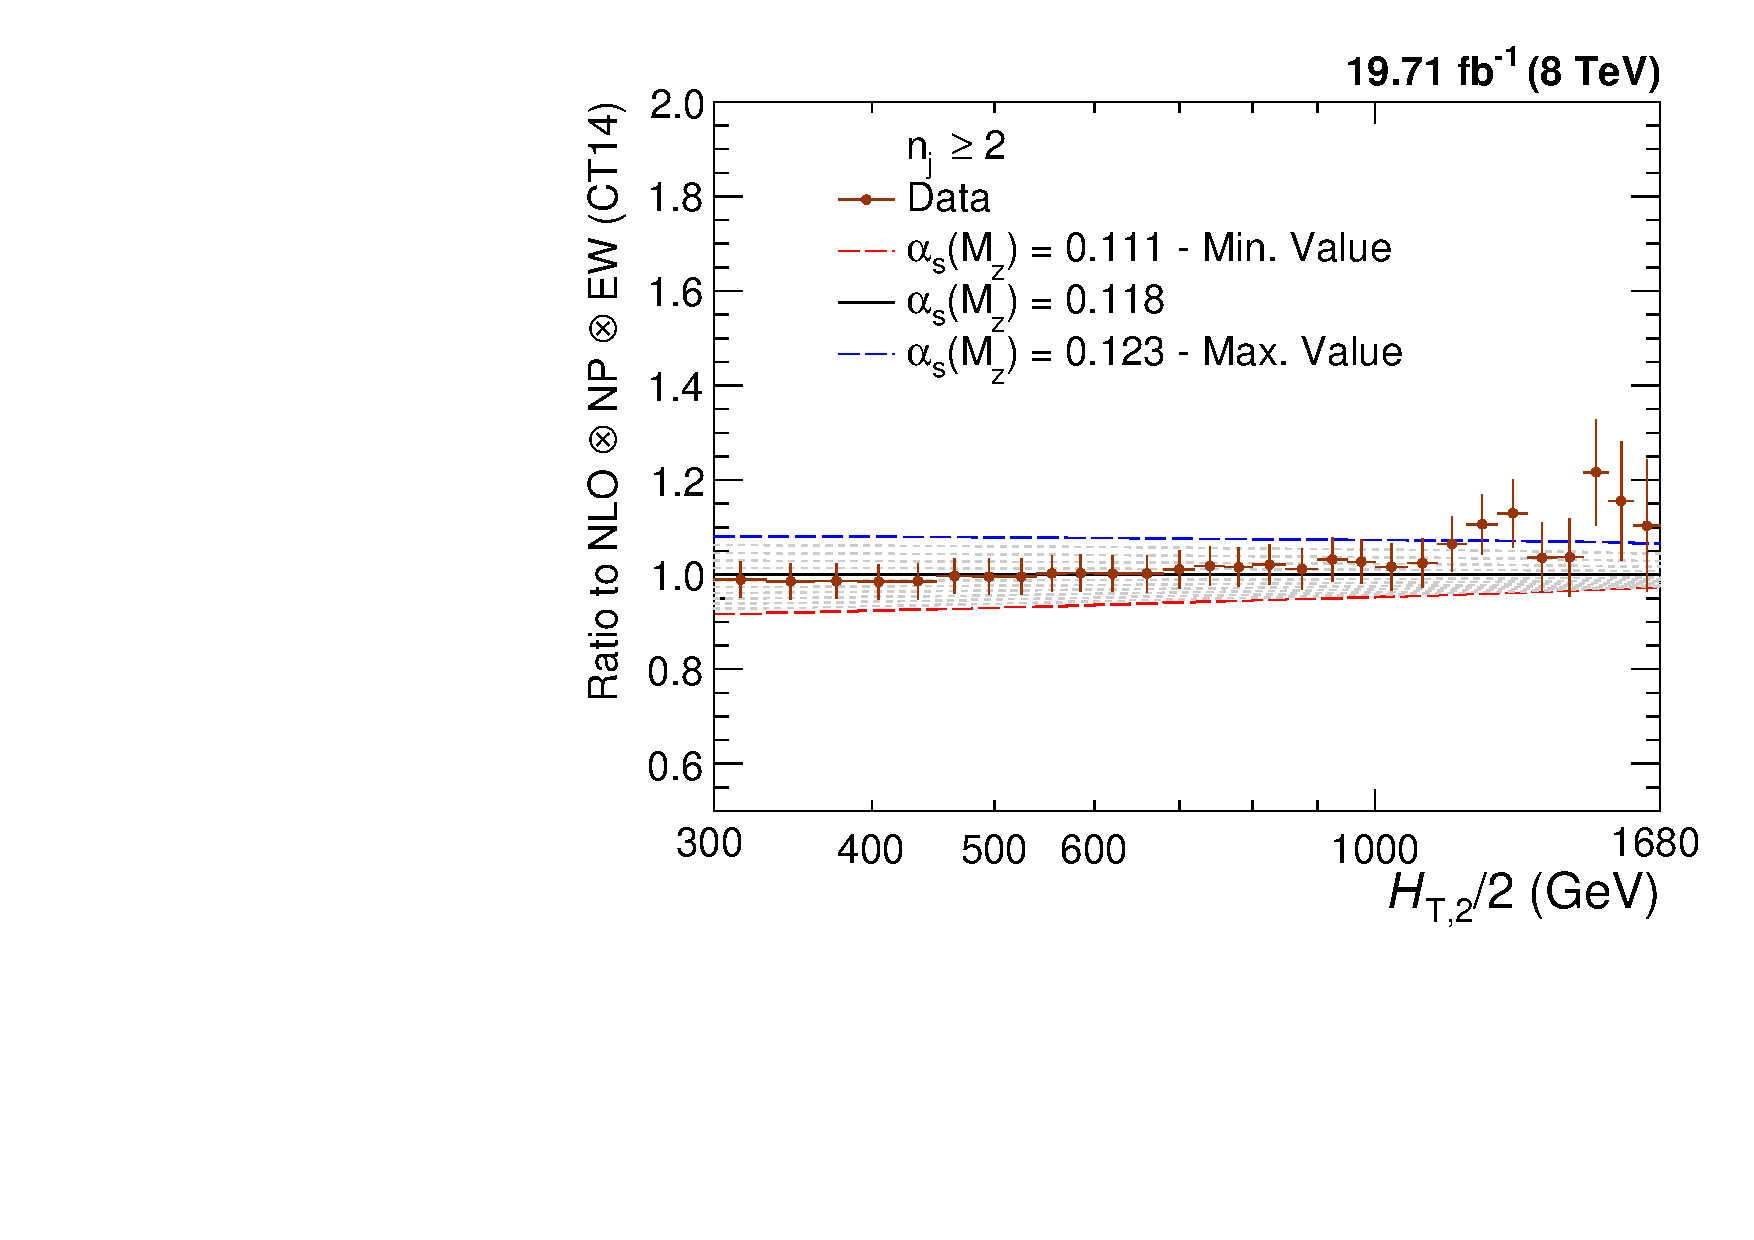
\includegraphics[width=0.51\textwidth]{Plots_HT_2_150/Sensitivity_2_ratio_NLO_CT14_EW.pdf}\\
 \vspace*{3mm}
 \hspace*{-5mm}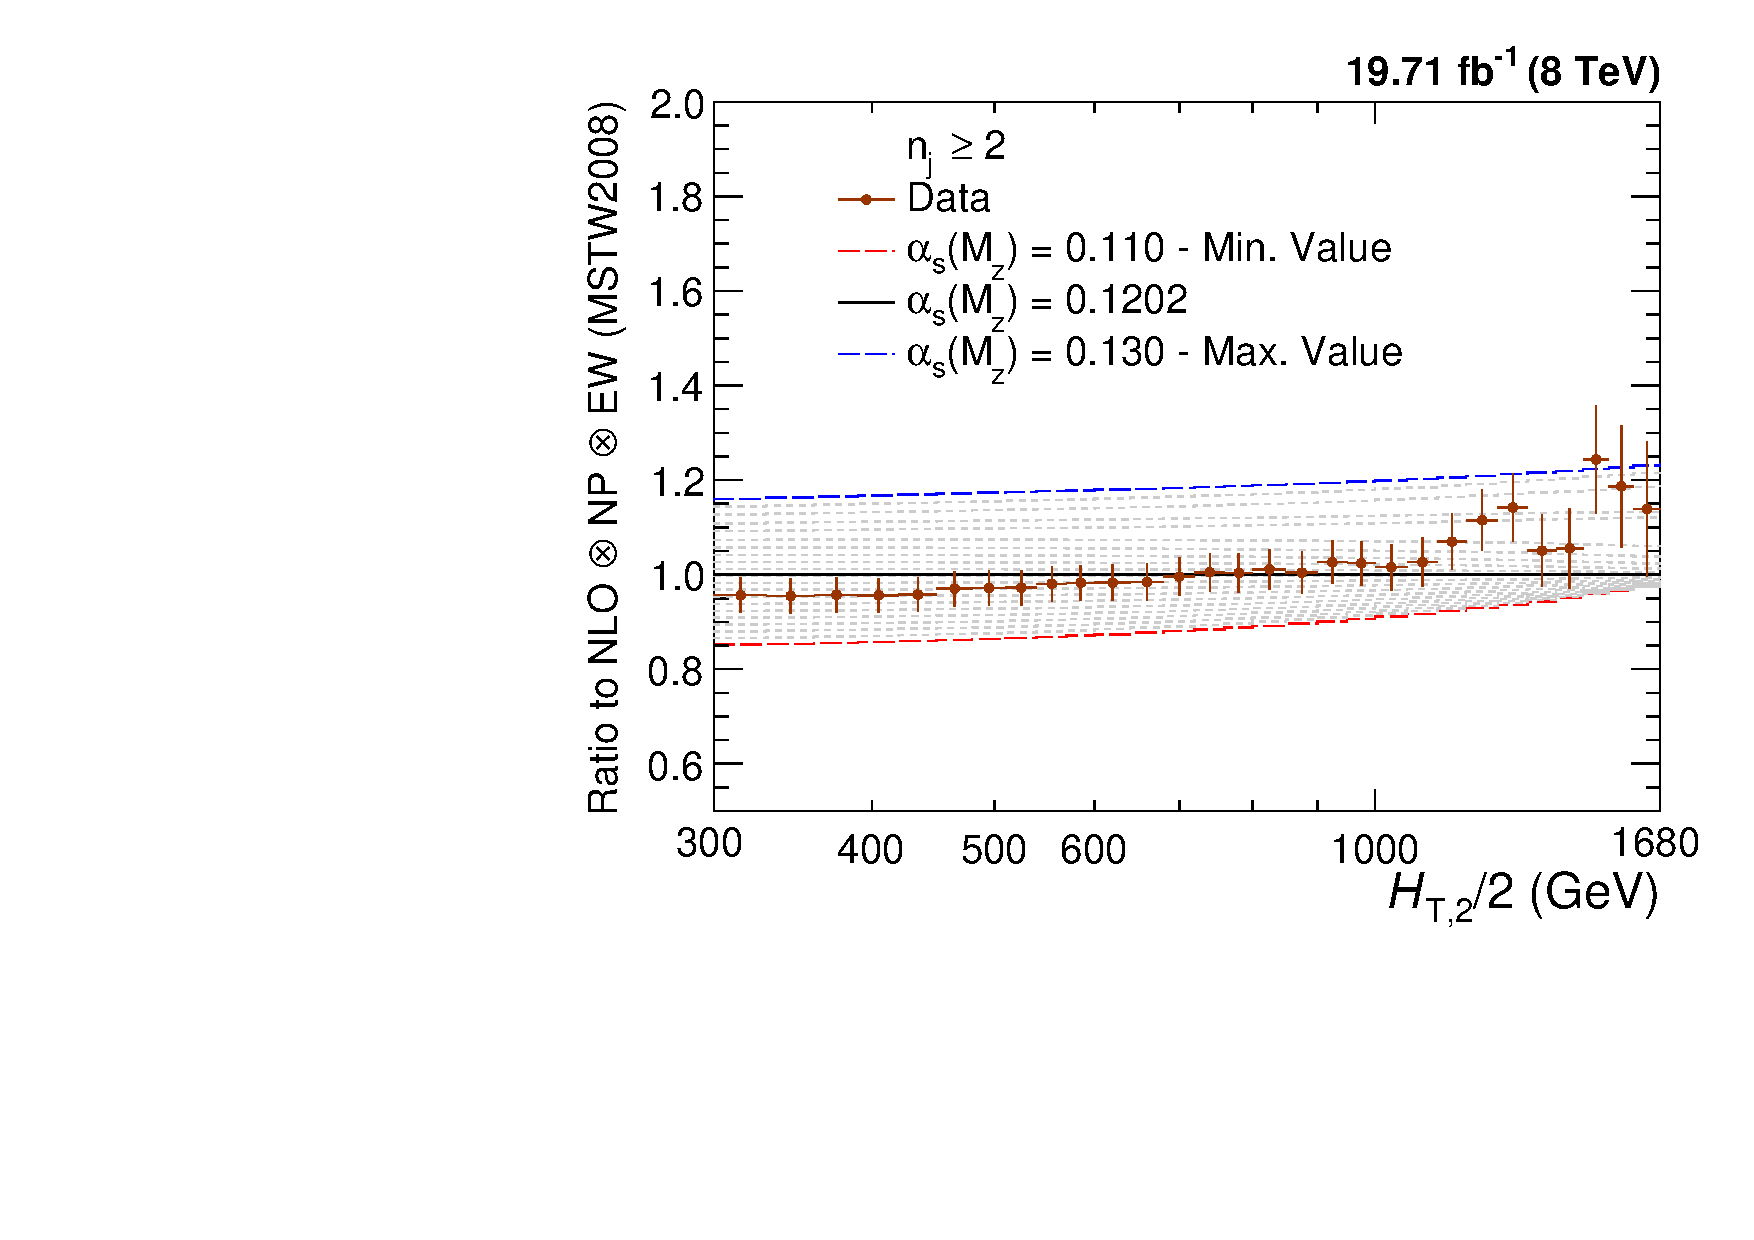
\includegraphics[width=0.51\textwidth]{Plots_HT_2_150/Sensitivity_2_ratio_NLO_MSTW2008_EW.pdf}%
 ~~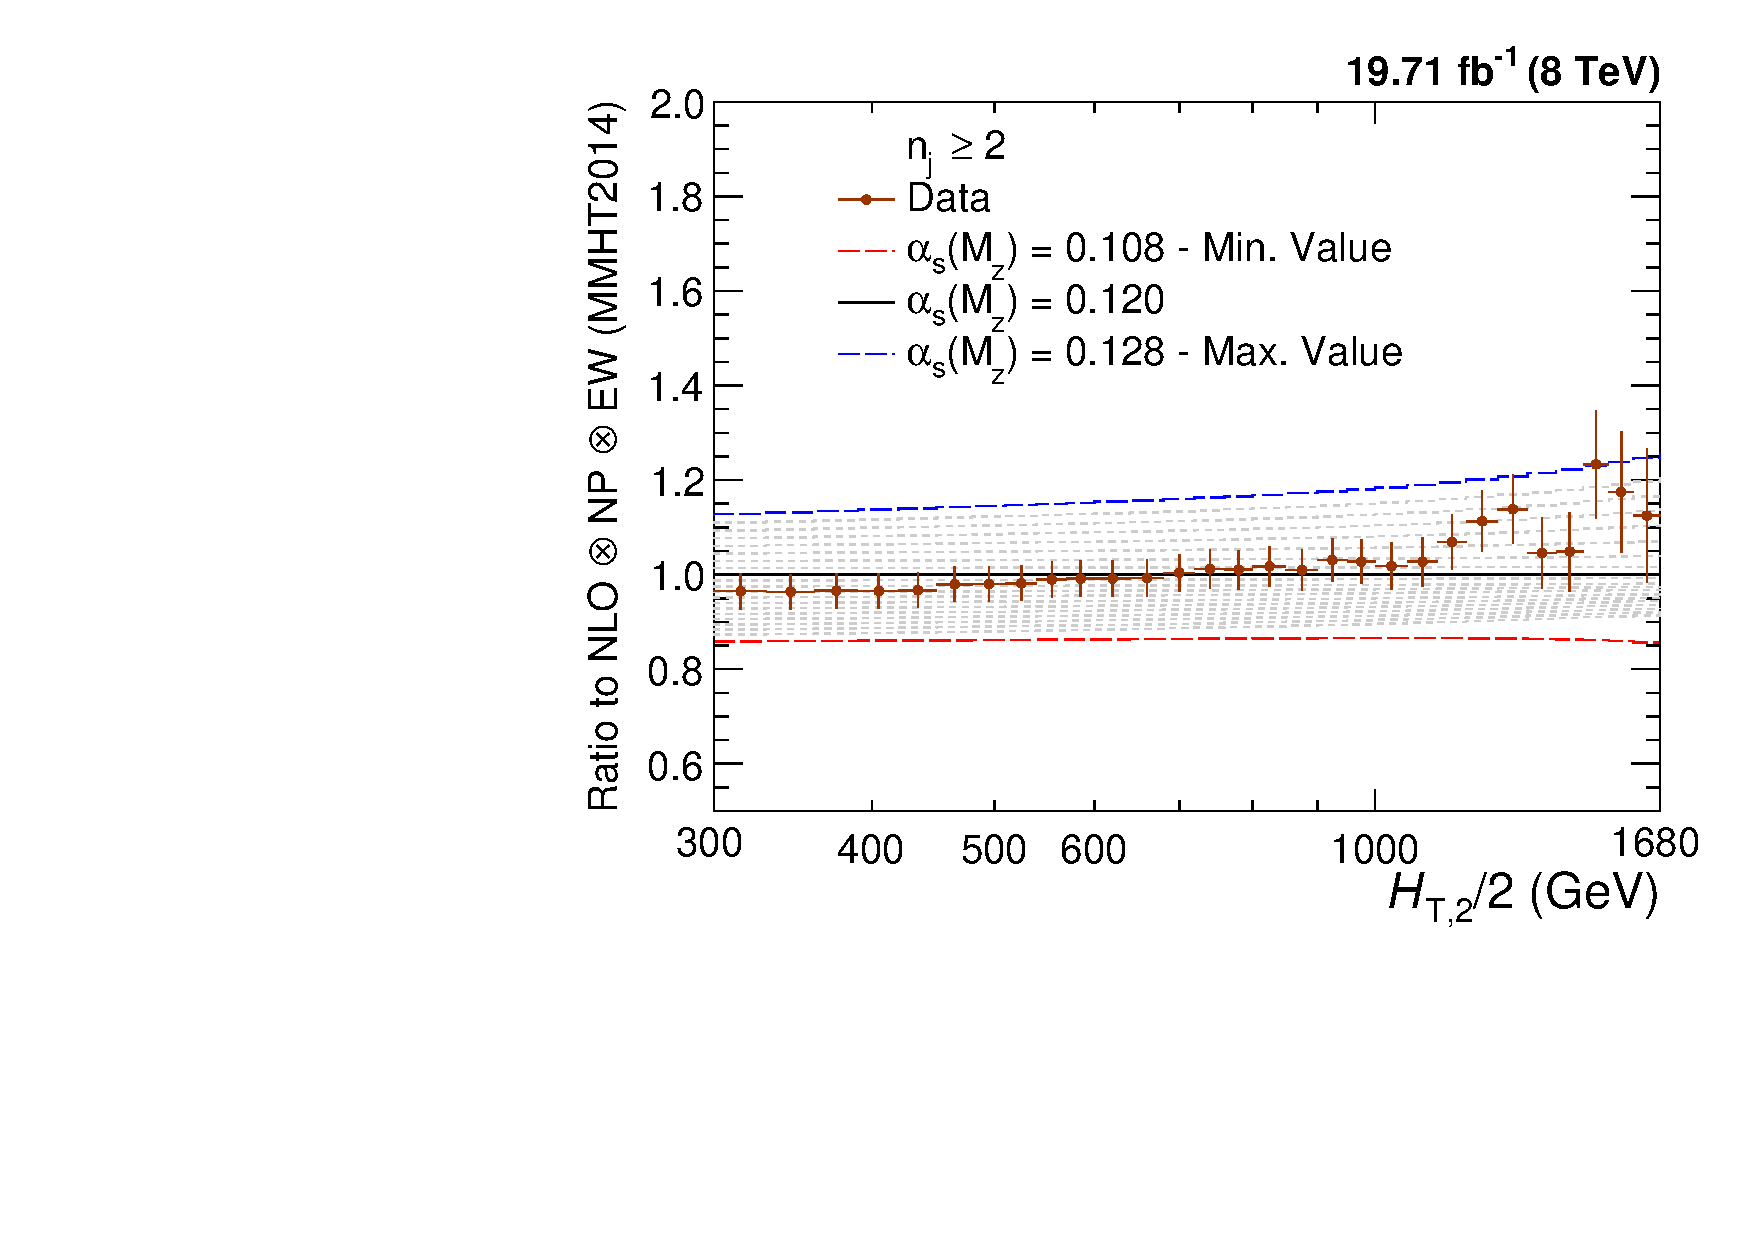
\includegraphics[width=0.51\textwidth]{Plots_HT_2_150/Sensitivity_2_ratio_NLO_MMHT2014_EW.pdf}\\
 \vspace*{3mm}
 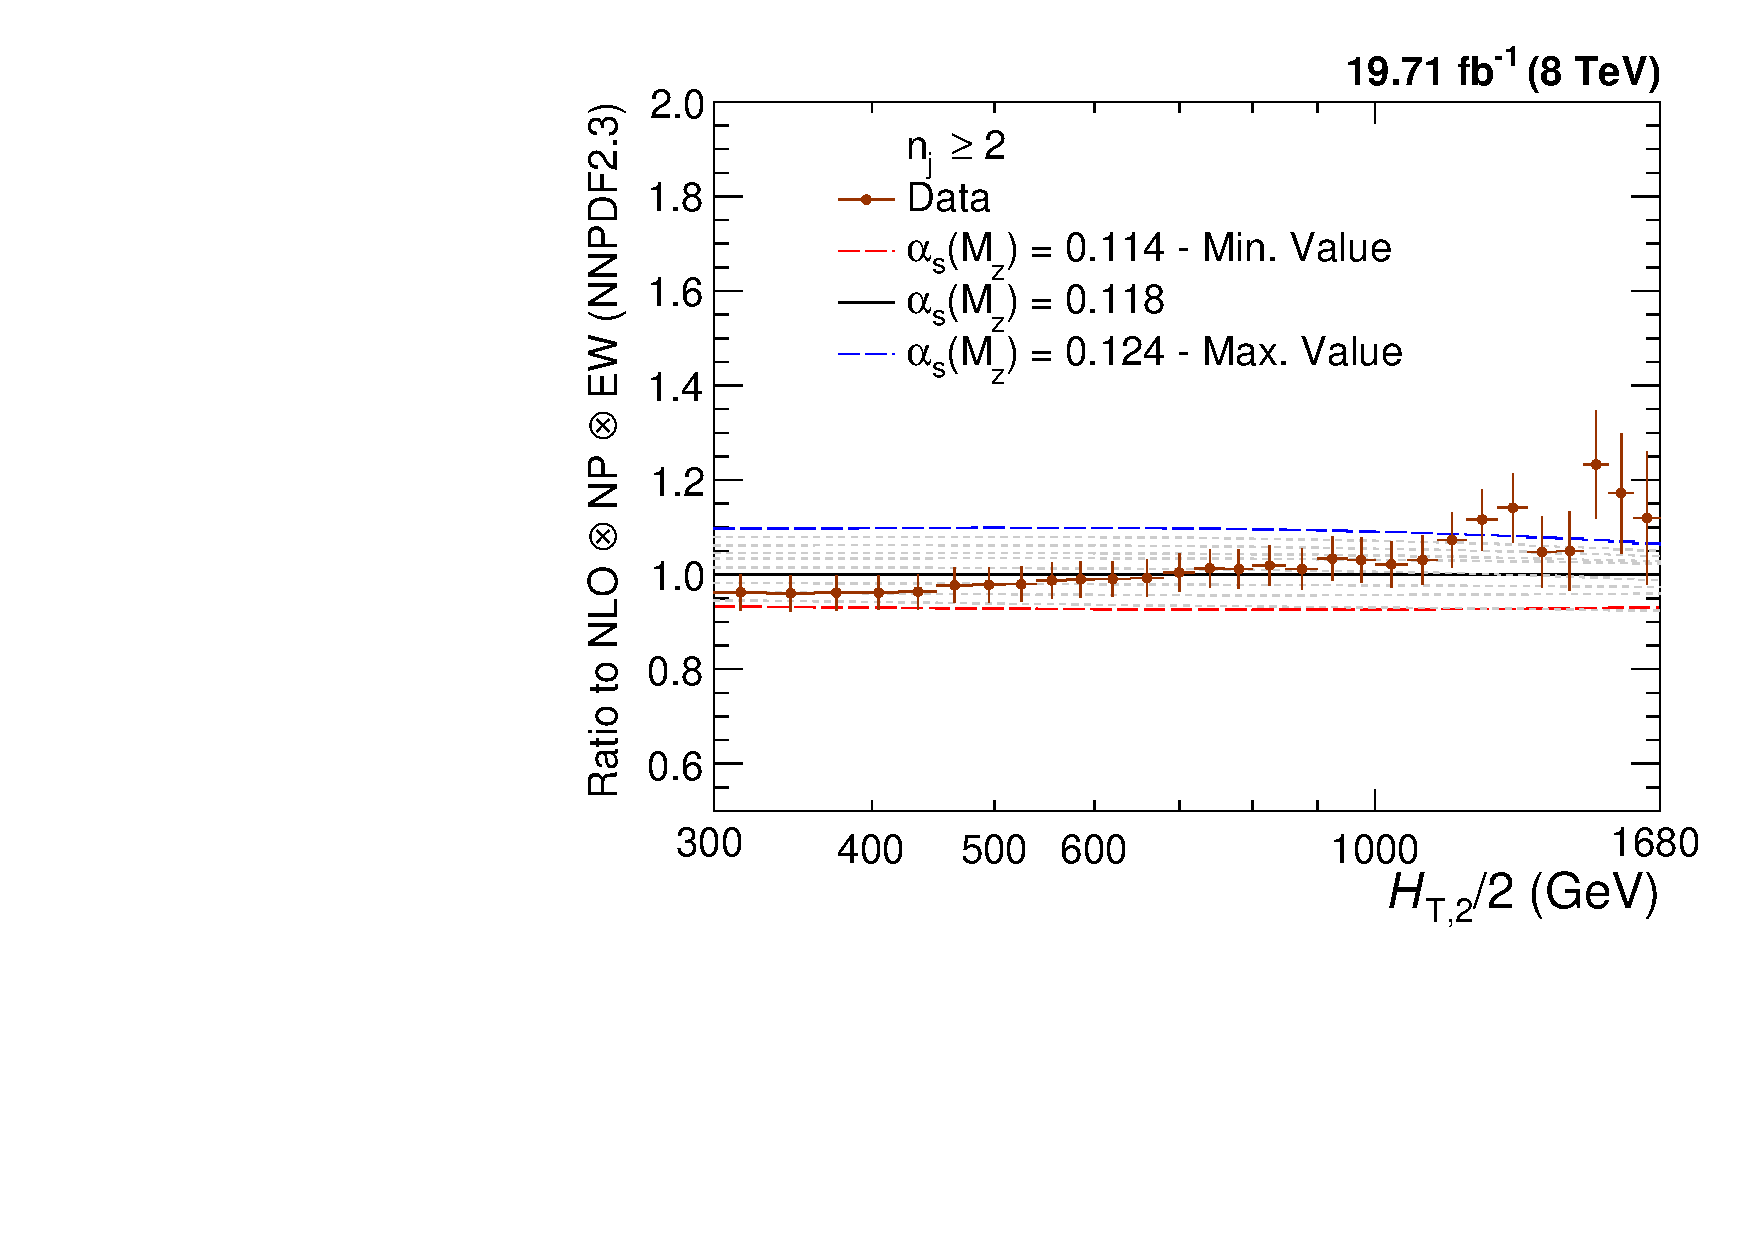
\includegraphics[width=0.51\textwidth]{Plots_HT_2_150/Sensitivity_2_ratio_NLO_NNPDF23_EW.pdf}
 \caption{Ratio of the inclusive 2-jet differential cross section to theory predictions using the CT10 (top left), the CT14 (top right), the MSTW2008 (middle left), the MMHT2014 (middle right) and NNPDF2.3 (bottom) NLO PDF sets for a series of values of \alpsmz. The \alpsmz value is varied in the range 0.112-0.127, 0.111-123, 0.110-0.130, 0.108-0.128 and 0.114-0.124 in steps of 0.001 for the CT10, CT14, MSTW2008, MMHT2014 and NNPDF2.3 NLO PDF sets, respectively. The error bars correspond to the total experimental uncertainty. The theory predictions are corrected for non-perturbative (NP) and electroweak (EW) effects.}
 \label{fig:sensitivity_2}
 \end{center}
\end{figure}

\begin{figure}[!htbp]
 \begin{center}
 \hspace*{-5mm}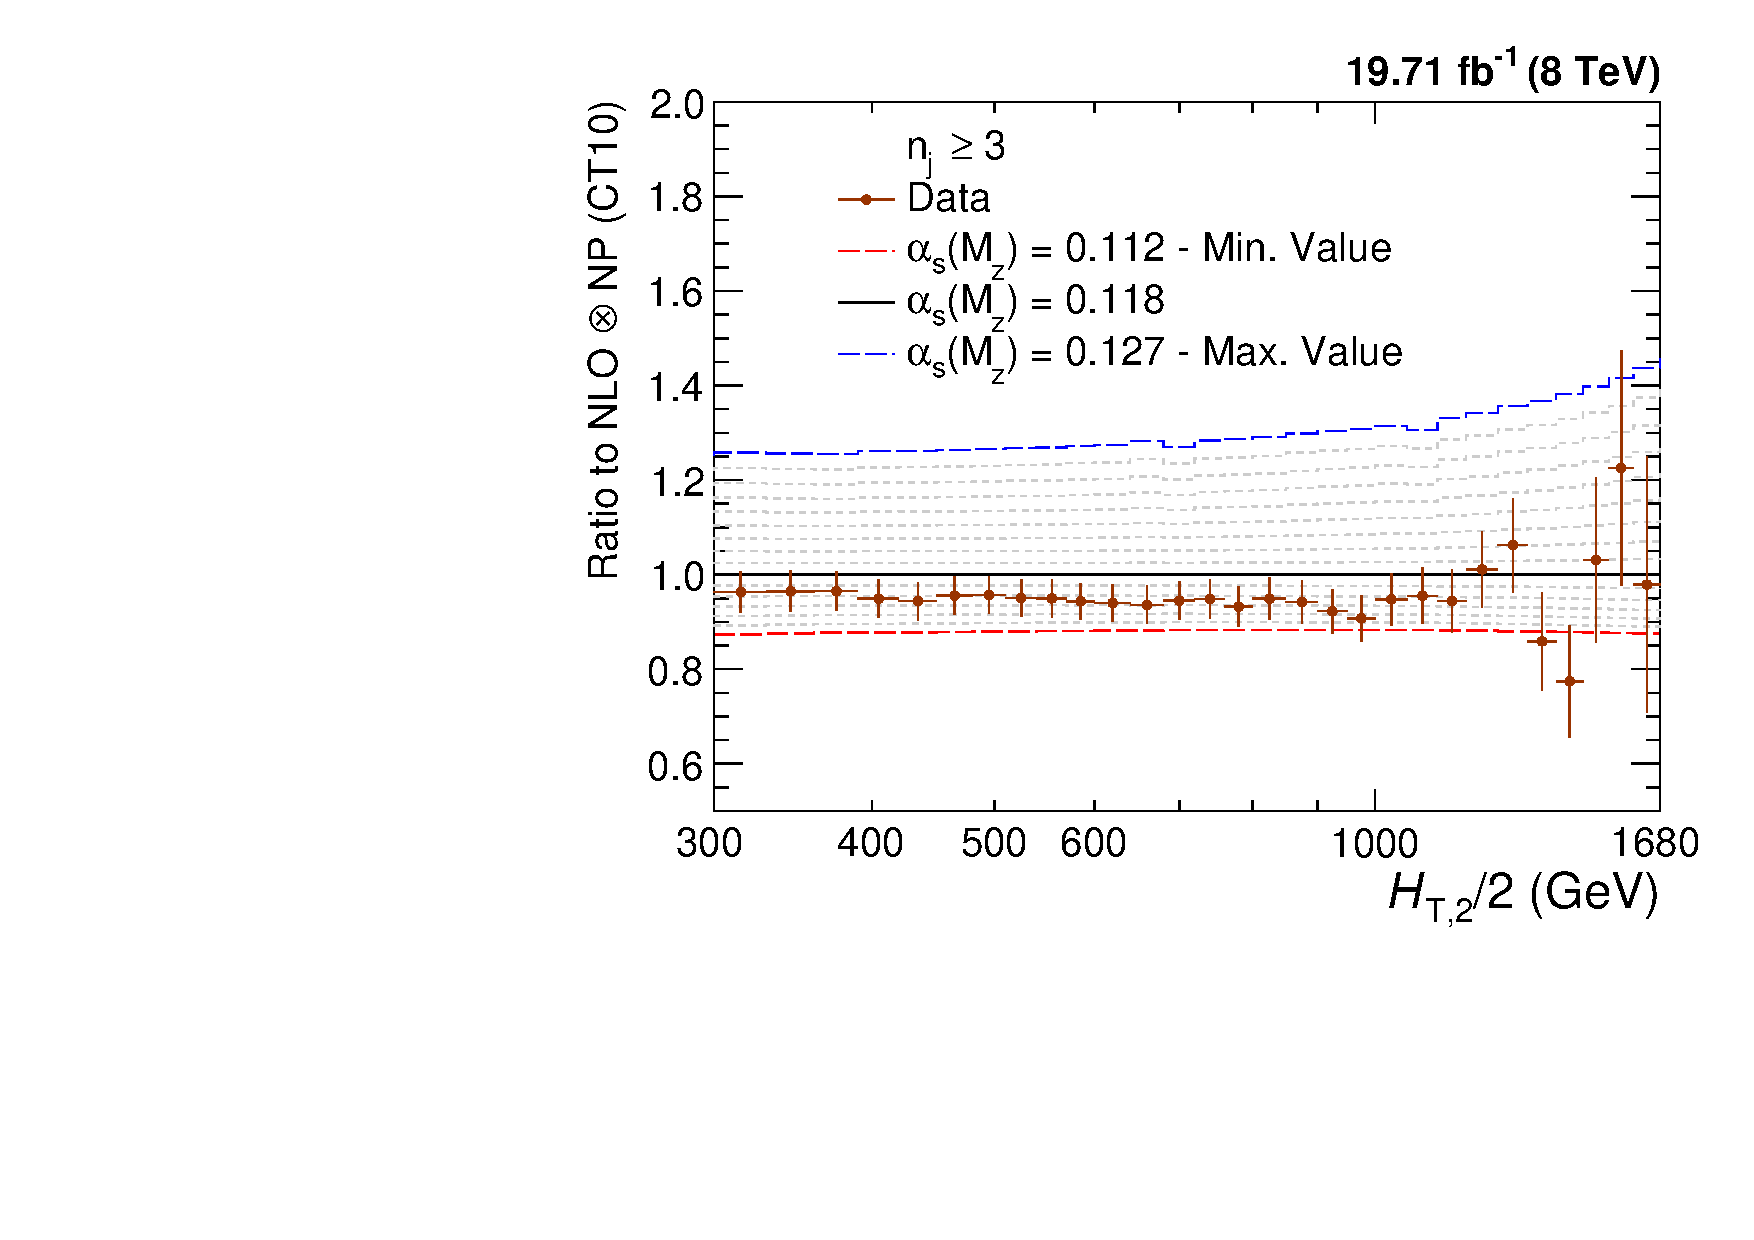
\includegraphics[width=0.51\textwidth]{Plots_HT_2_150/Sensitivity_3_ratio_NLO_CT10.pdf}%
 ~~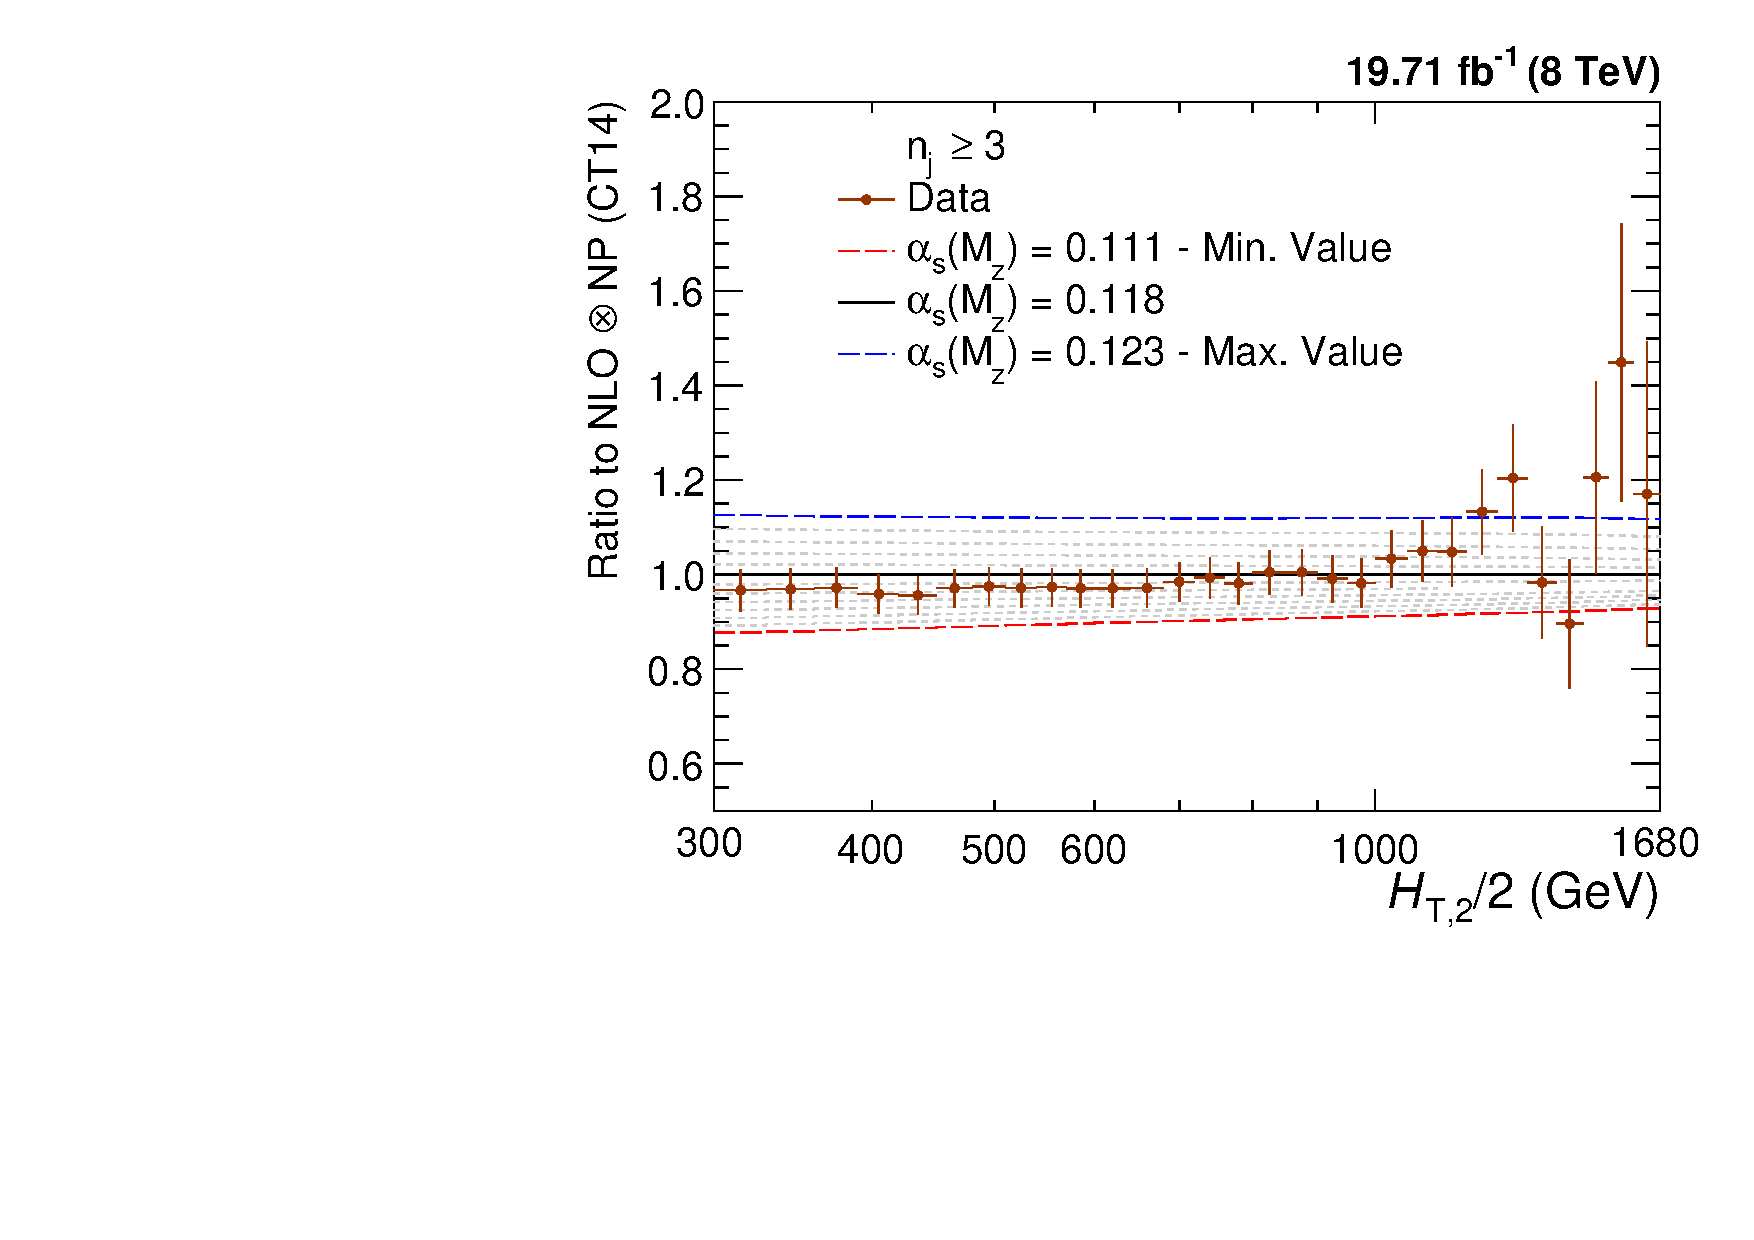
\includegraphics[width=0.51\textwidth]{Plots_HT_2_150/Sensitivity_3_ratio_NLO_CT14.pdf}\\
 \vspace*{3mm}
 \hspace*{-5mm}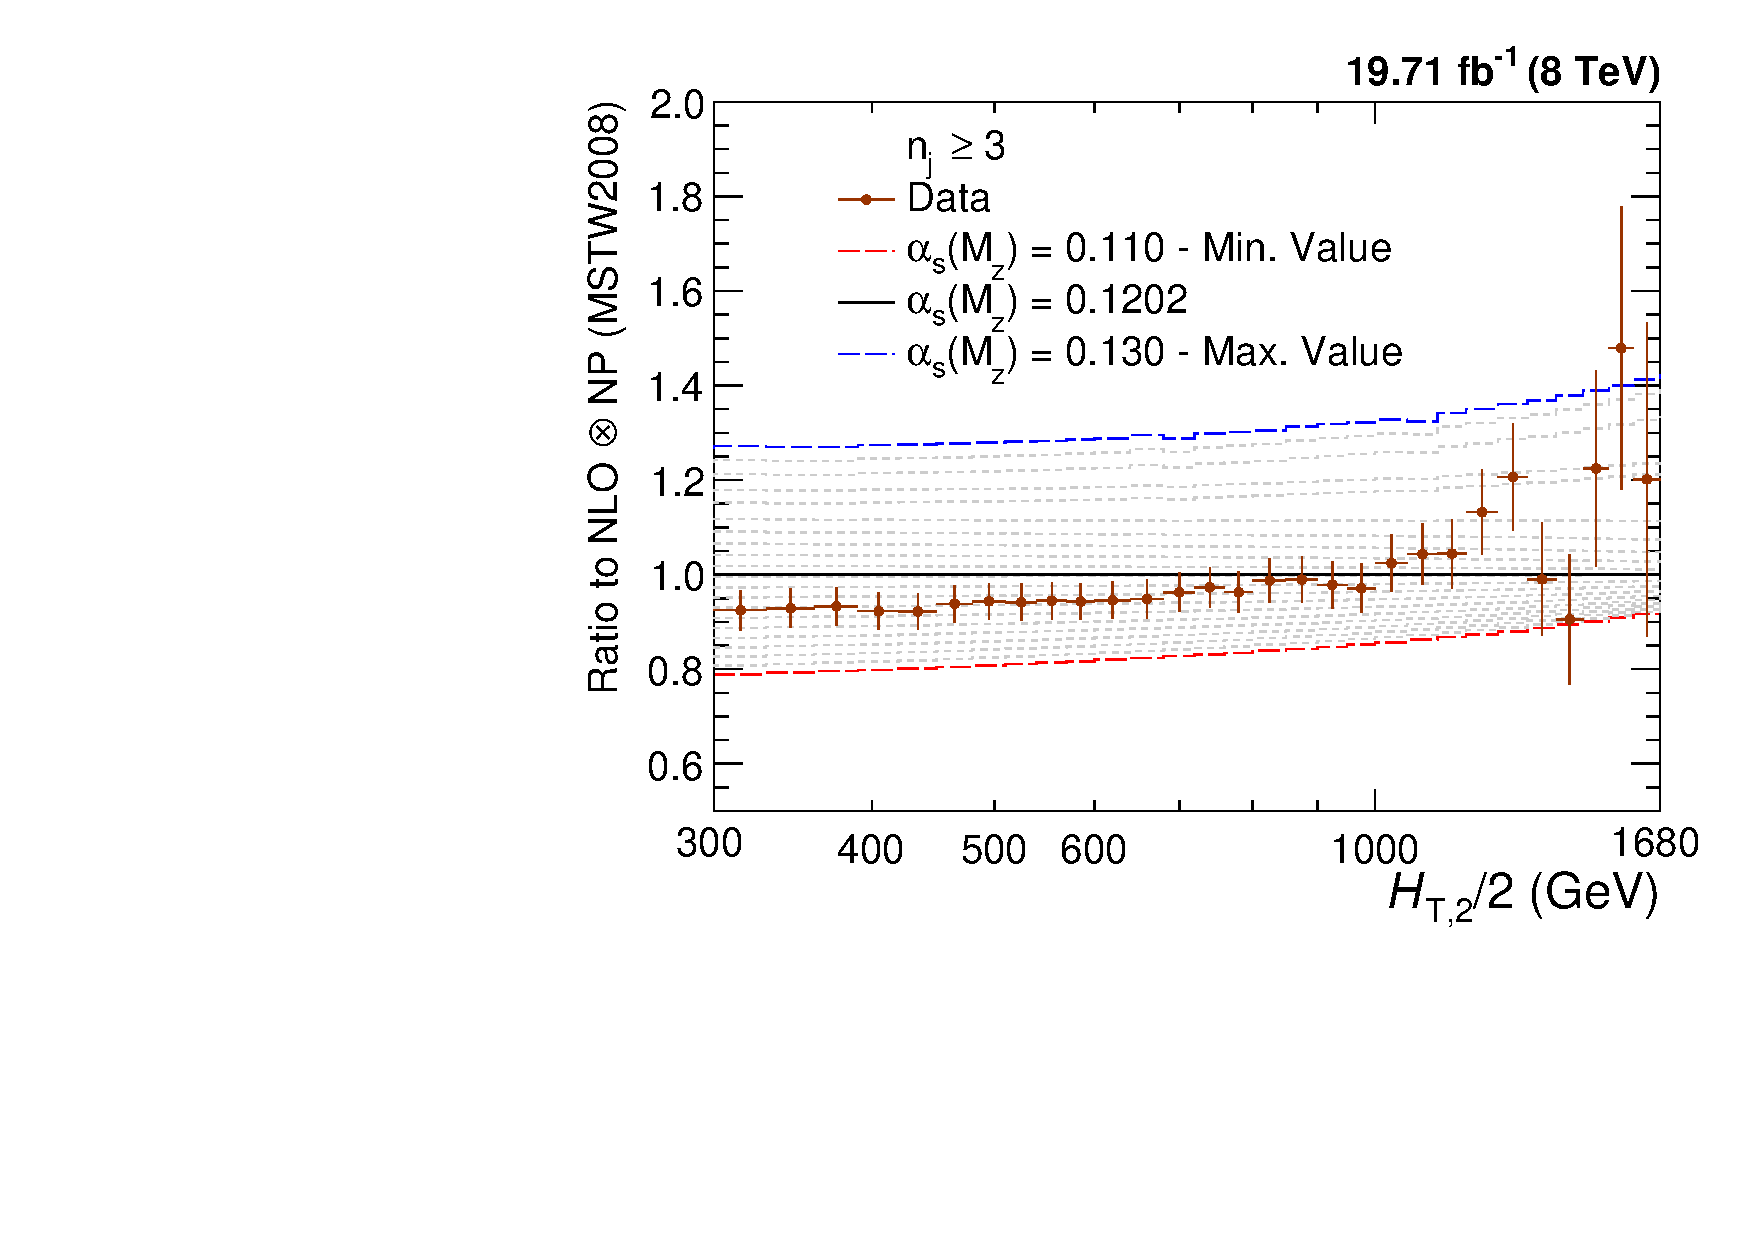
\includegraphics[width=0.51\textwidth]{Plots_HT_2_150/Sensitivity_3_ratio_NLO_MSTW2008.pdf}%
 ~~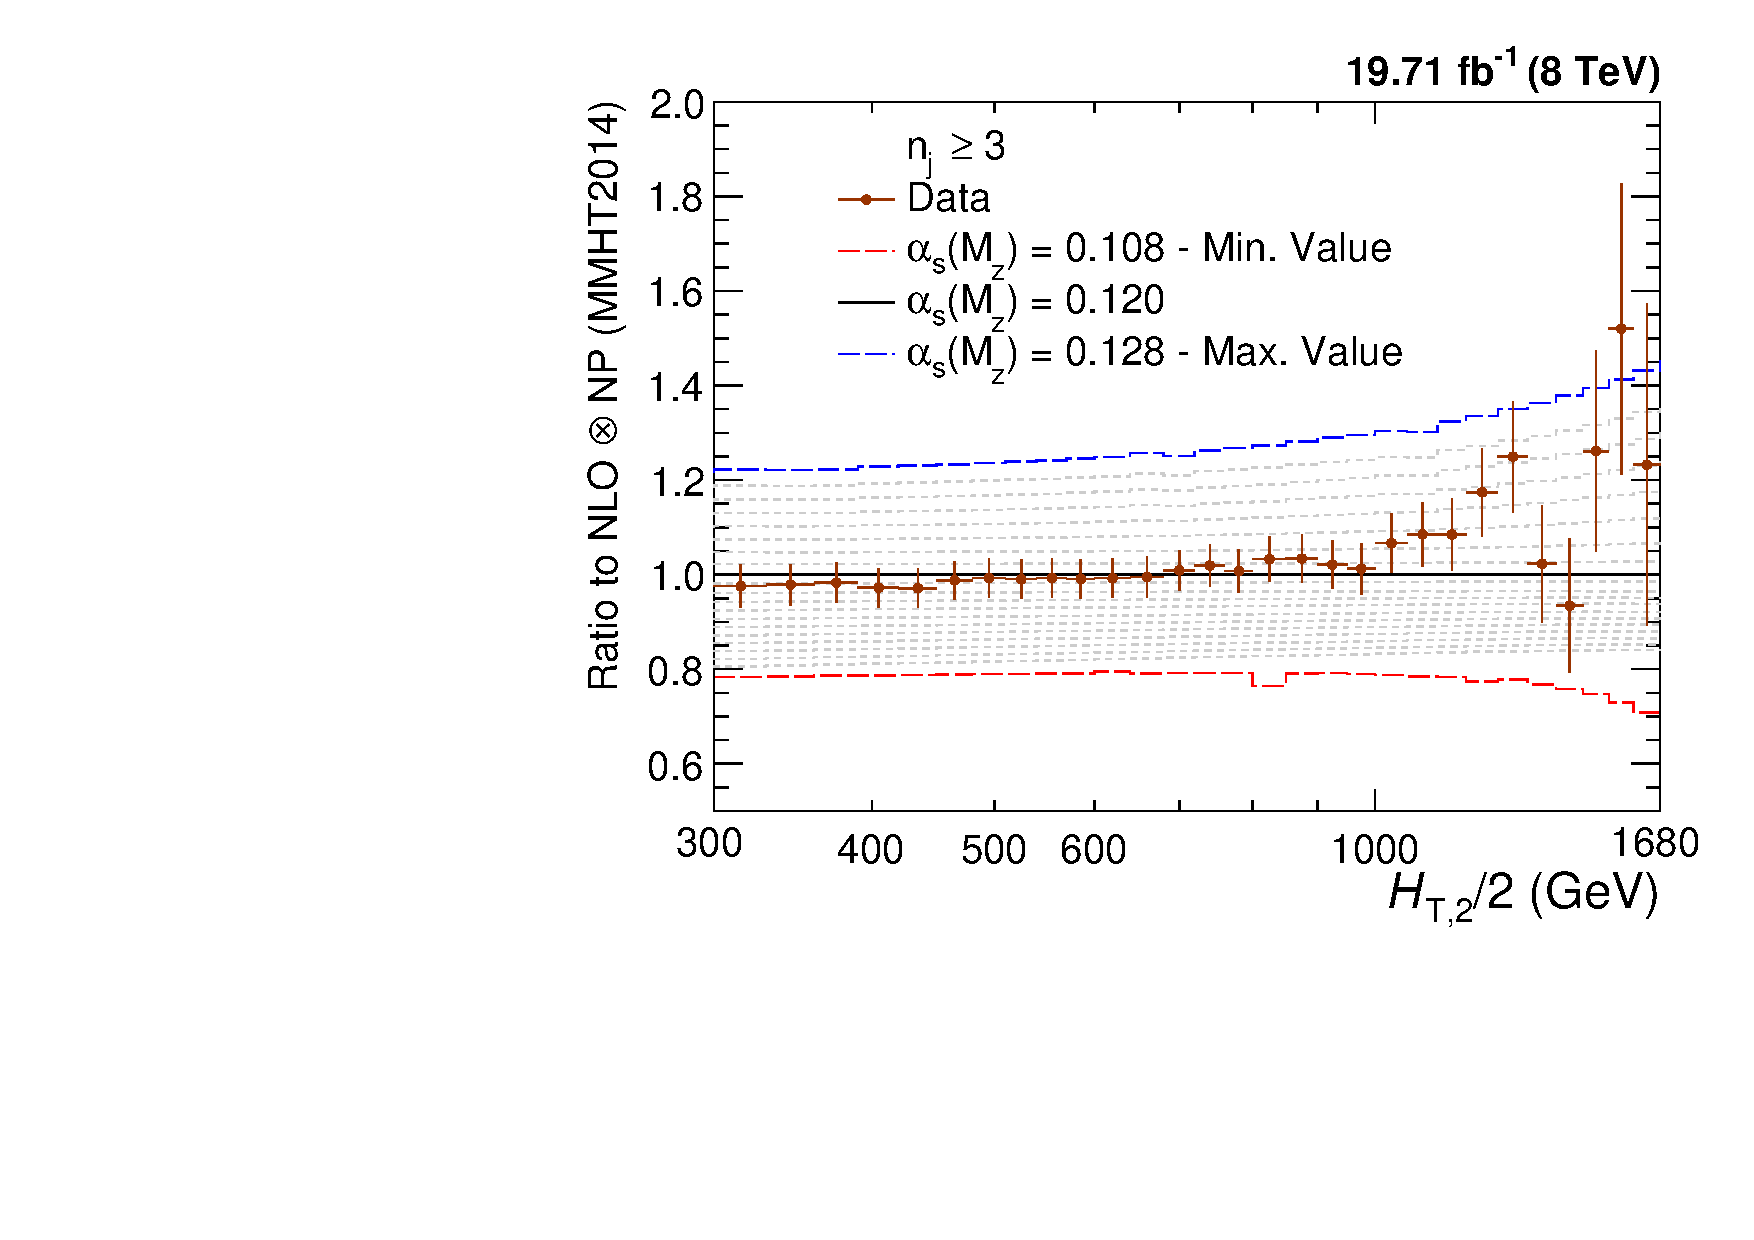
\includegraphics[width=0.51\textwidth]{Plots_HT_2_150/Sensitivity_3_ratio_NLO_MMHT2014.pdf}\\
 \vspace*{3mm}
 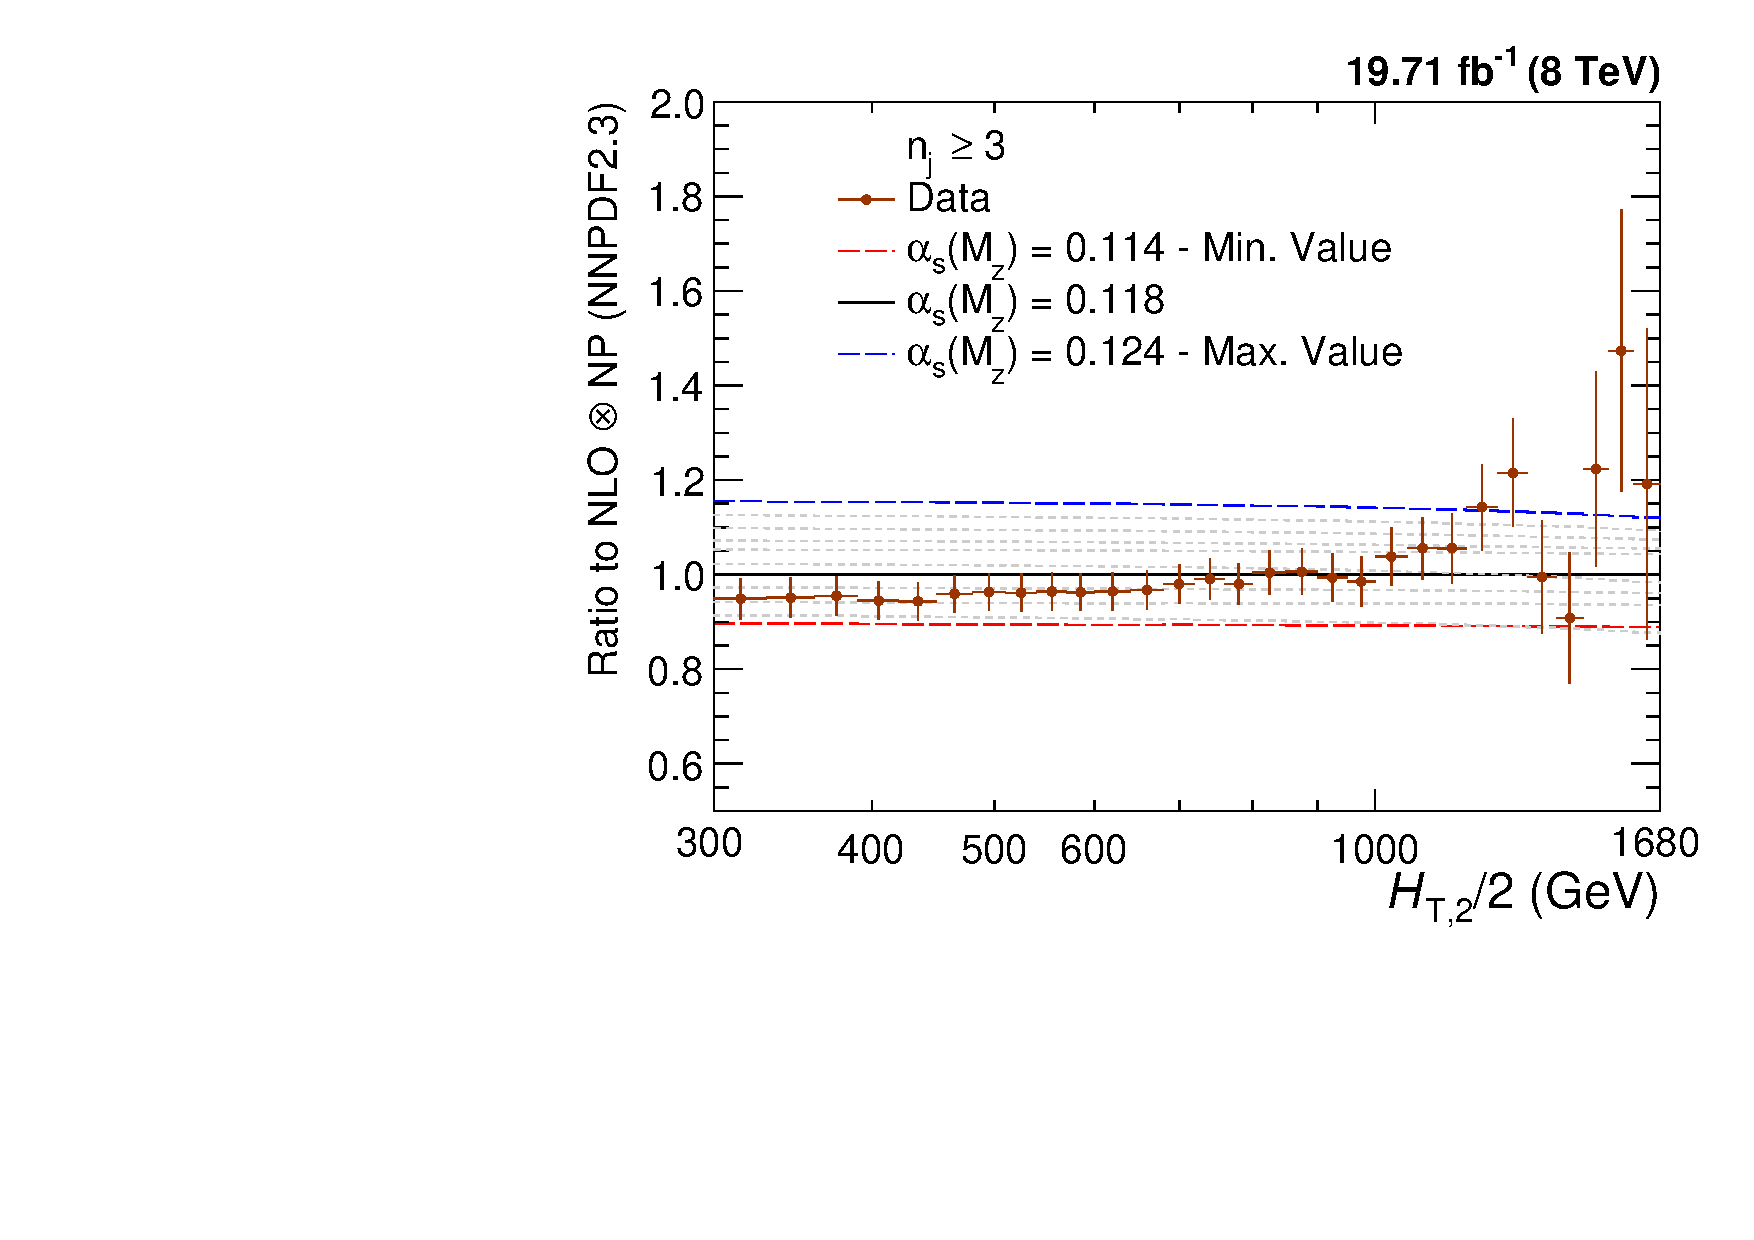
\includegraphics[width=0.51\textwidth]{Plots_HT_2_150/Sensitivity_3_ratio_NLO_NNPDF23.pdf}
 \caption{Ratio of the inclusive 3-jet differential cross section to theory predictions using the CT10 (top left), the CT14 (top right), the MSTW2008 (middle left), the MMHT2014 (middle right) and NNPDF2.3 (bottom) NLO PDF sets for a series of values of \alpsmz. The \alpsmz value is varied in the range 0.112-0.127, 0.111-123, 0.110-0.130, 0.108-0.128 and 0.114-0.124 in steps of 0.001 for the CT10, CT14, MSTW2008, MMHT2014 and NNPDF2.3 NLO PDF sets, respectively. The error bars correspond to the total experimental uncertainty. The theory predictions are corrected for non-perturbative (NP) effects.}
 \label{fig:sensitivity_3}
 \end{center}
\end{figure}

\begin{figure}[!htbp]
 \begin{center}
 \hspace*{-5mm}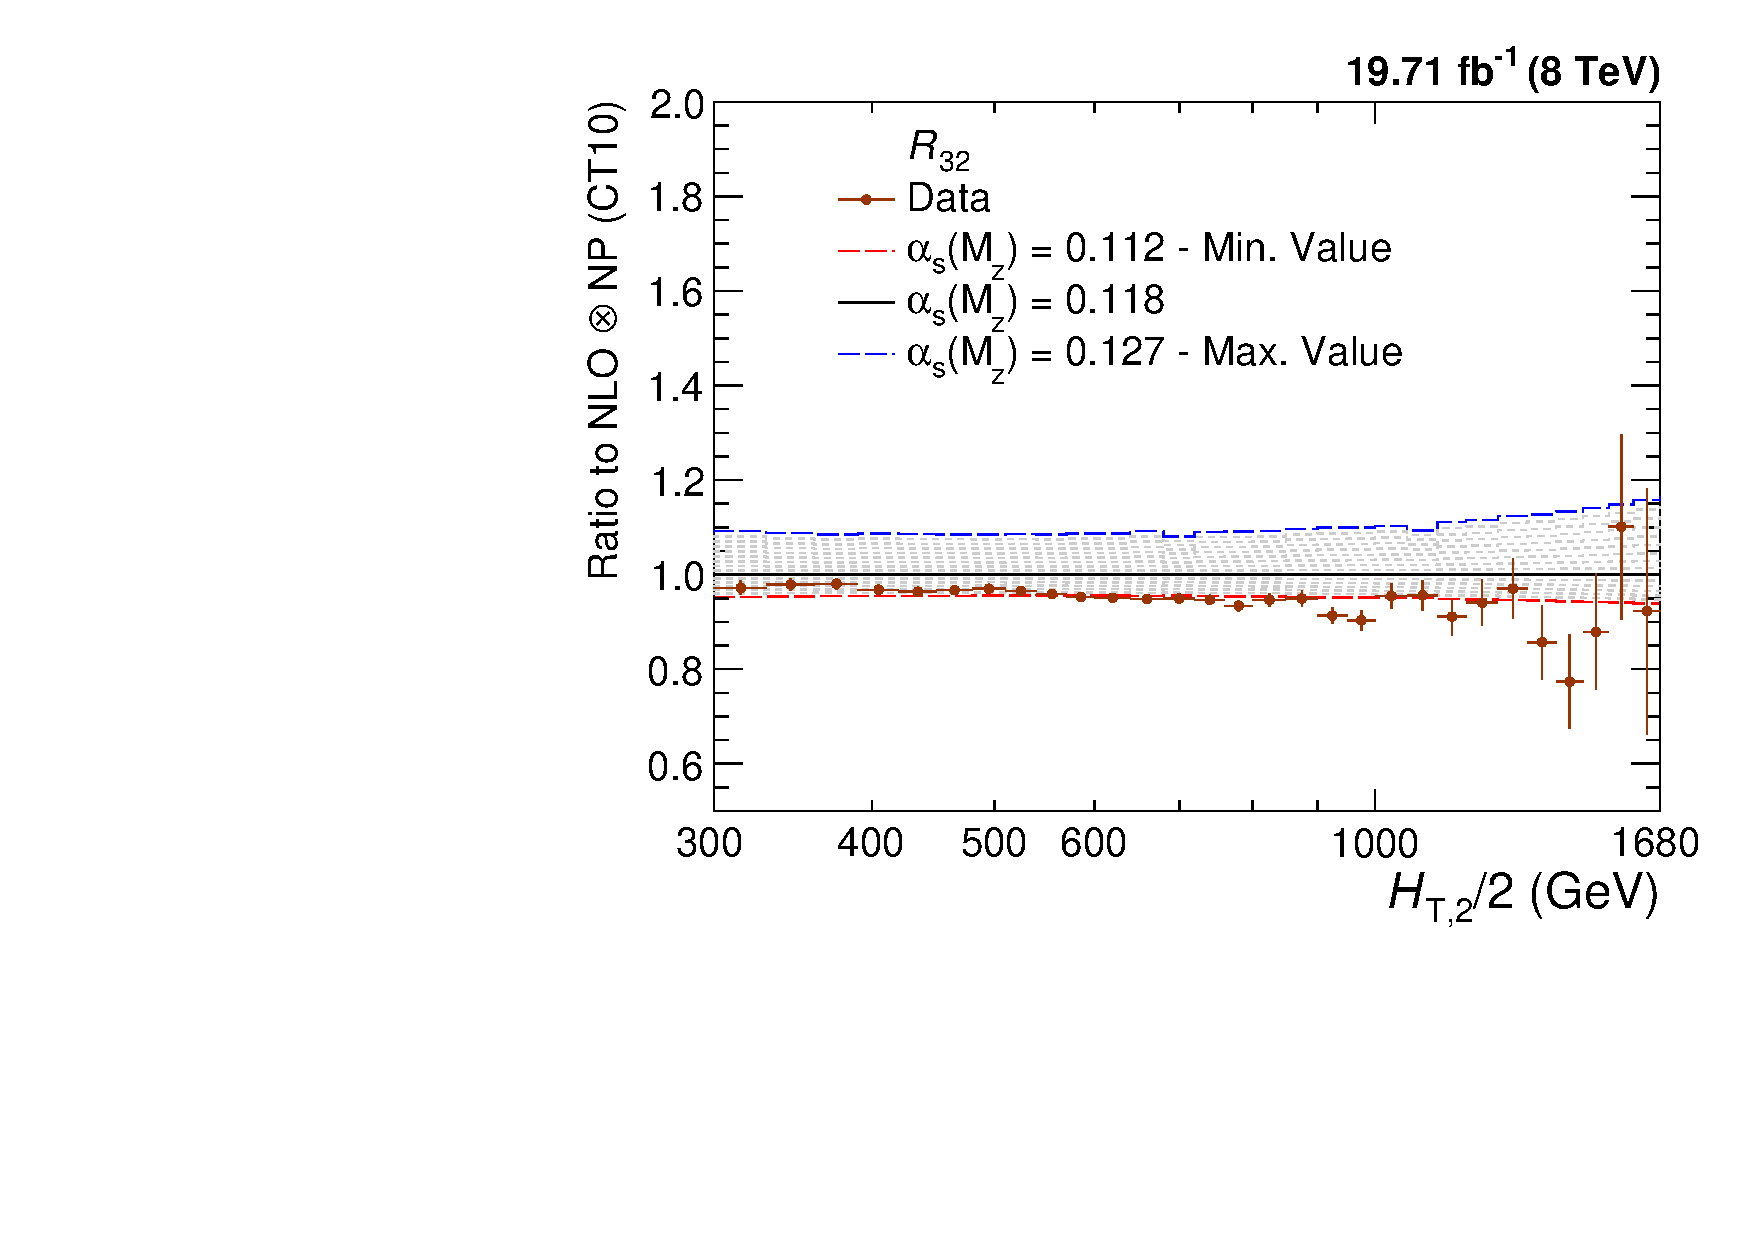
\includegraphics[width=0.51\textwidth]{Plots_HT_2_150/Sensitivity_double_ratio_32_CT10.pdf}%
 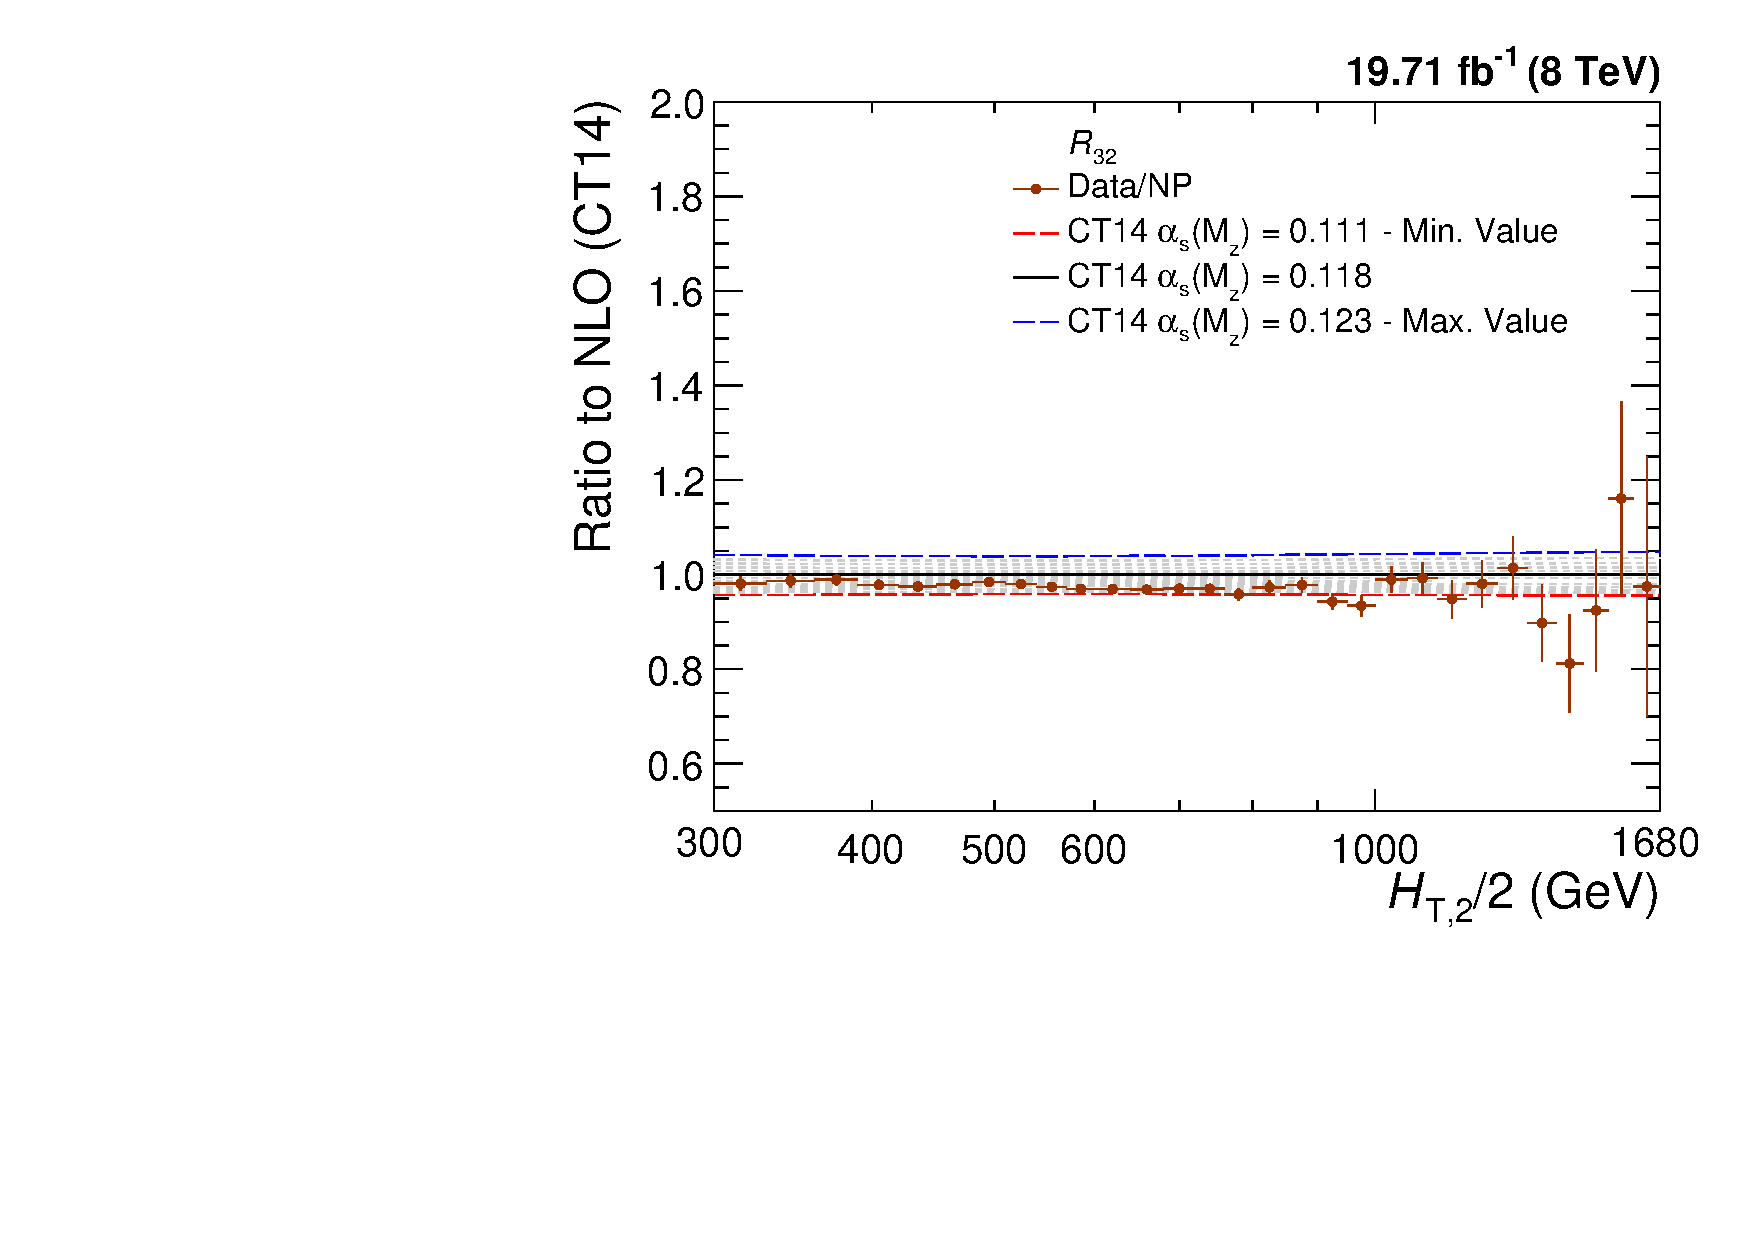
\includegraphics[width=0.51\textwidth]{Plots_HT_2_150/Sensitivity_double_ratio_32_CT14.pdf}\\
 \vspace*{3mm}
 \hspace*{-5mm}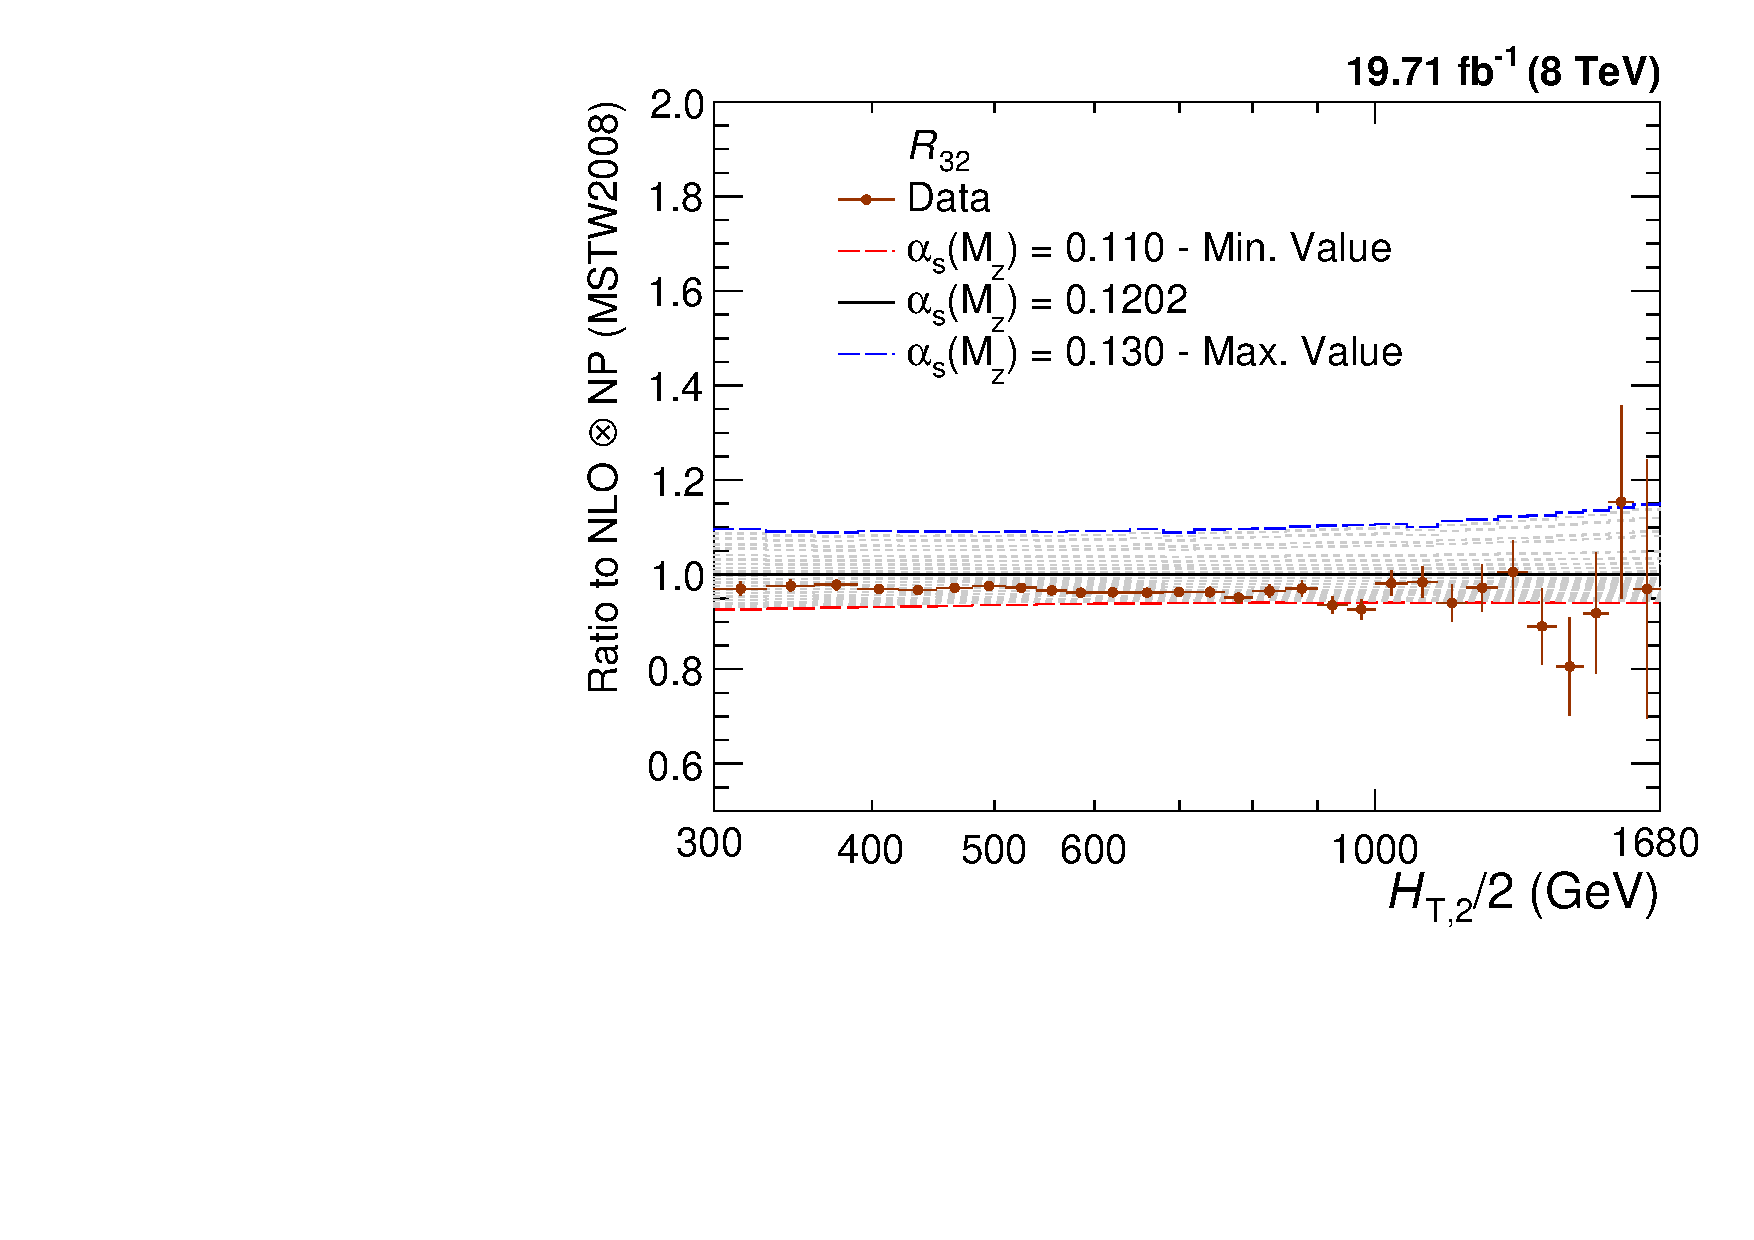
\includegraphics[width=0.51\textwidth]{Plots_HT_2_150/Sensitivity_double_ratio_32_MSTW2008.pdf}%
 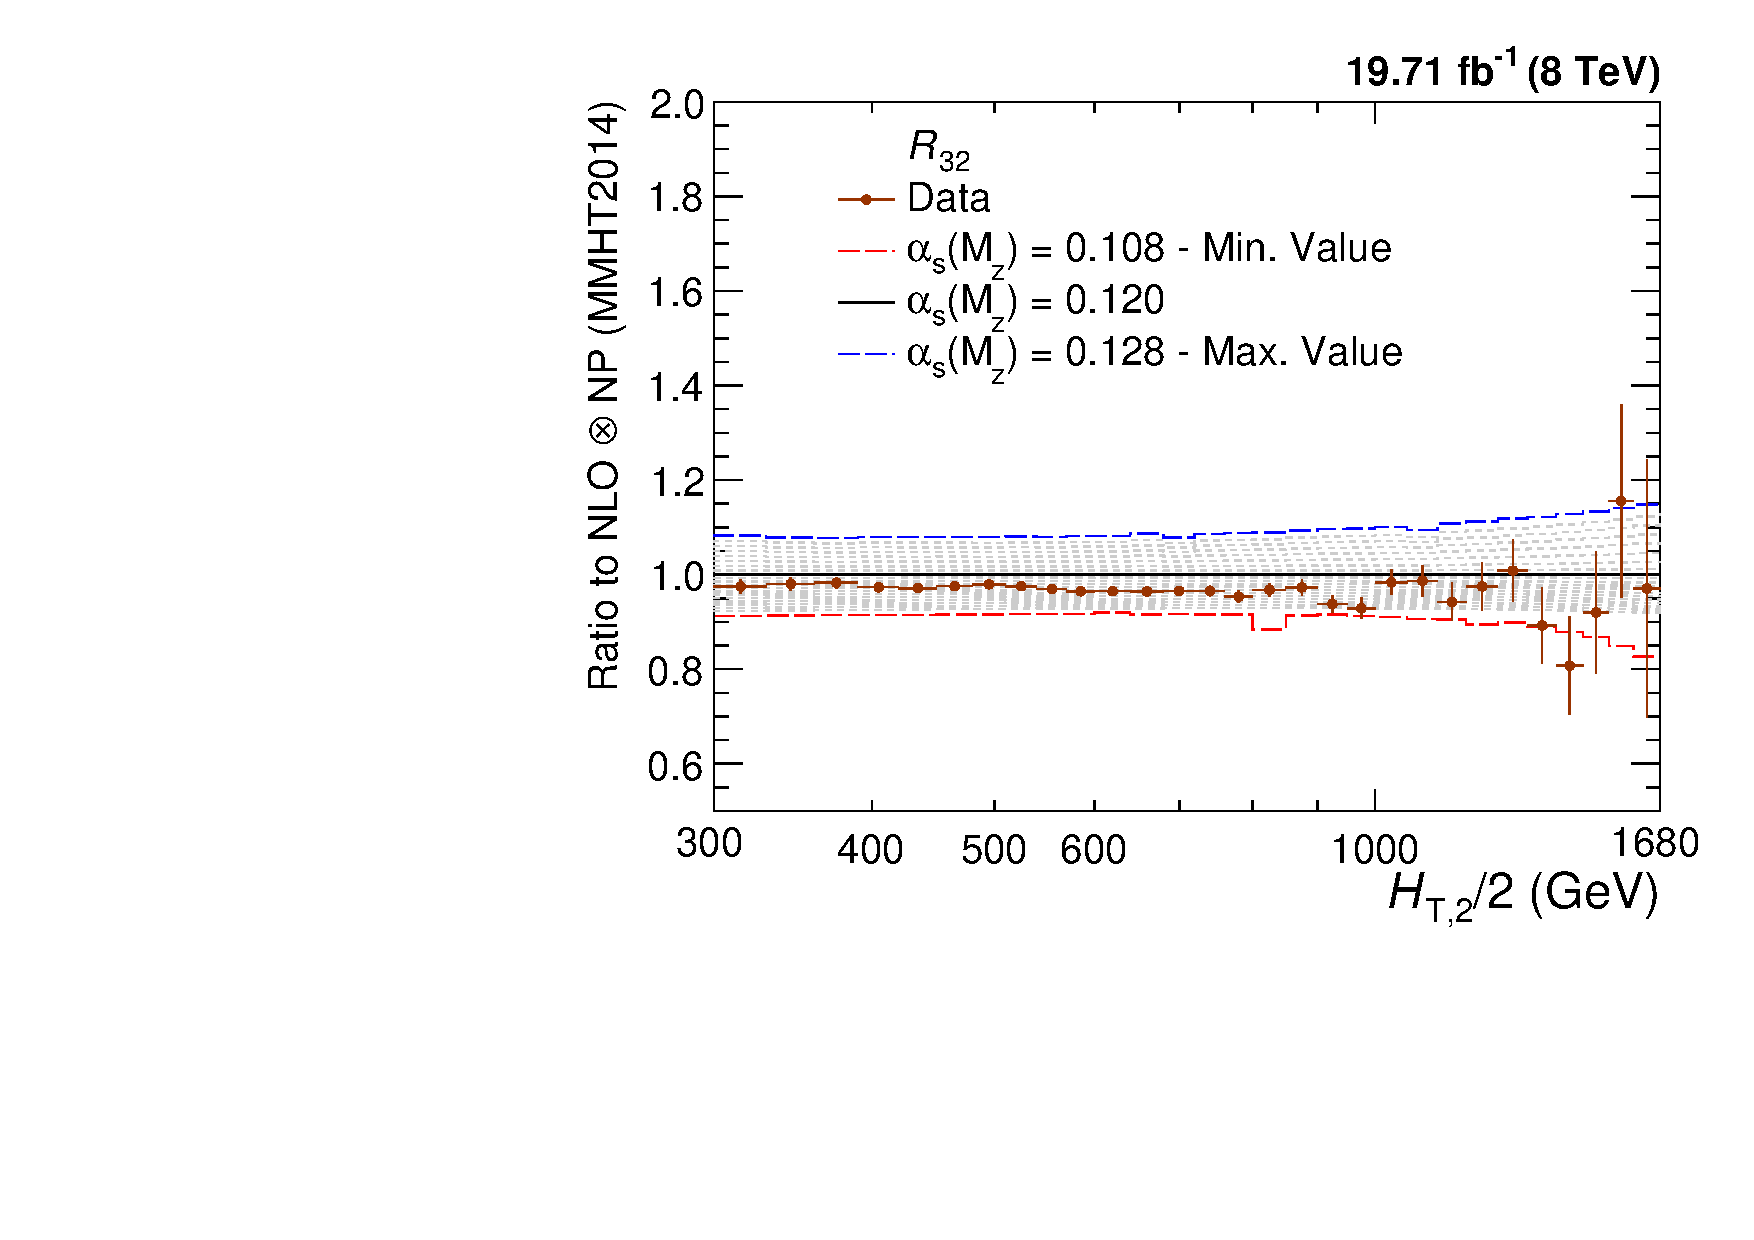
\includegraphics[width=0.51\textwidth]{Plots_HT_2_150/Sensitivity_double_ratio_32_MMHT2014.pdf}\\
 \vspace*{3mm}
 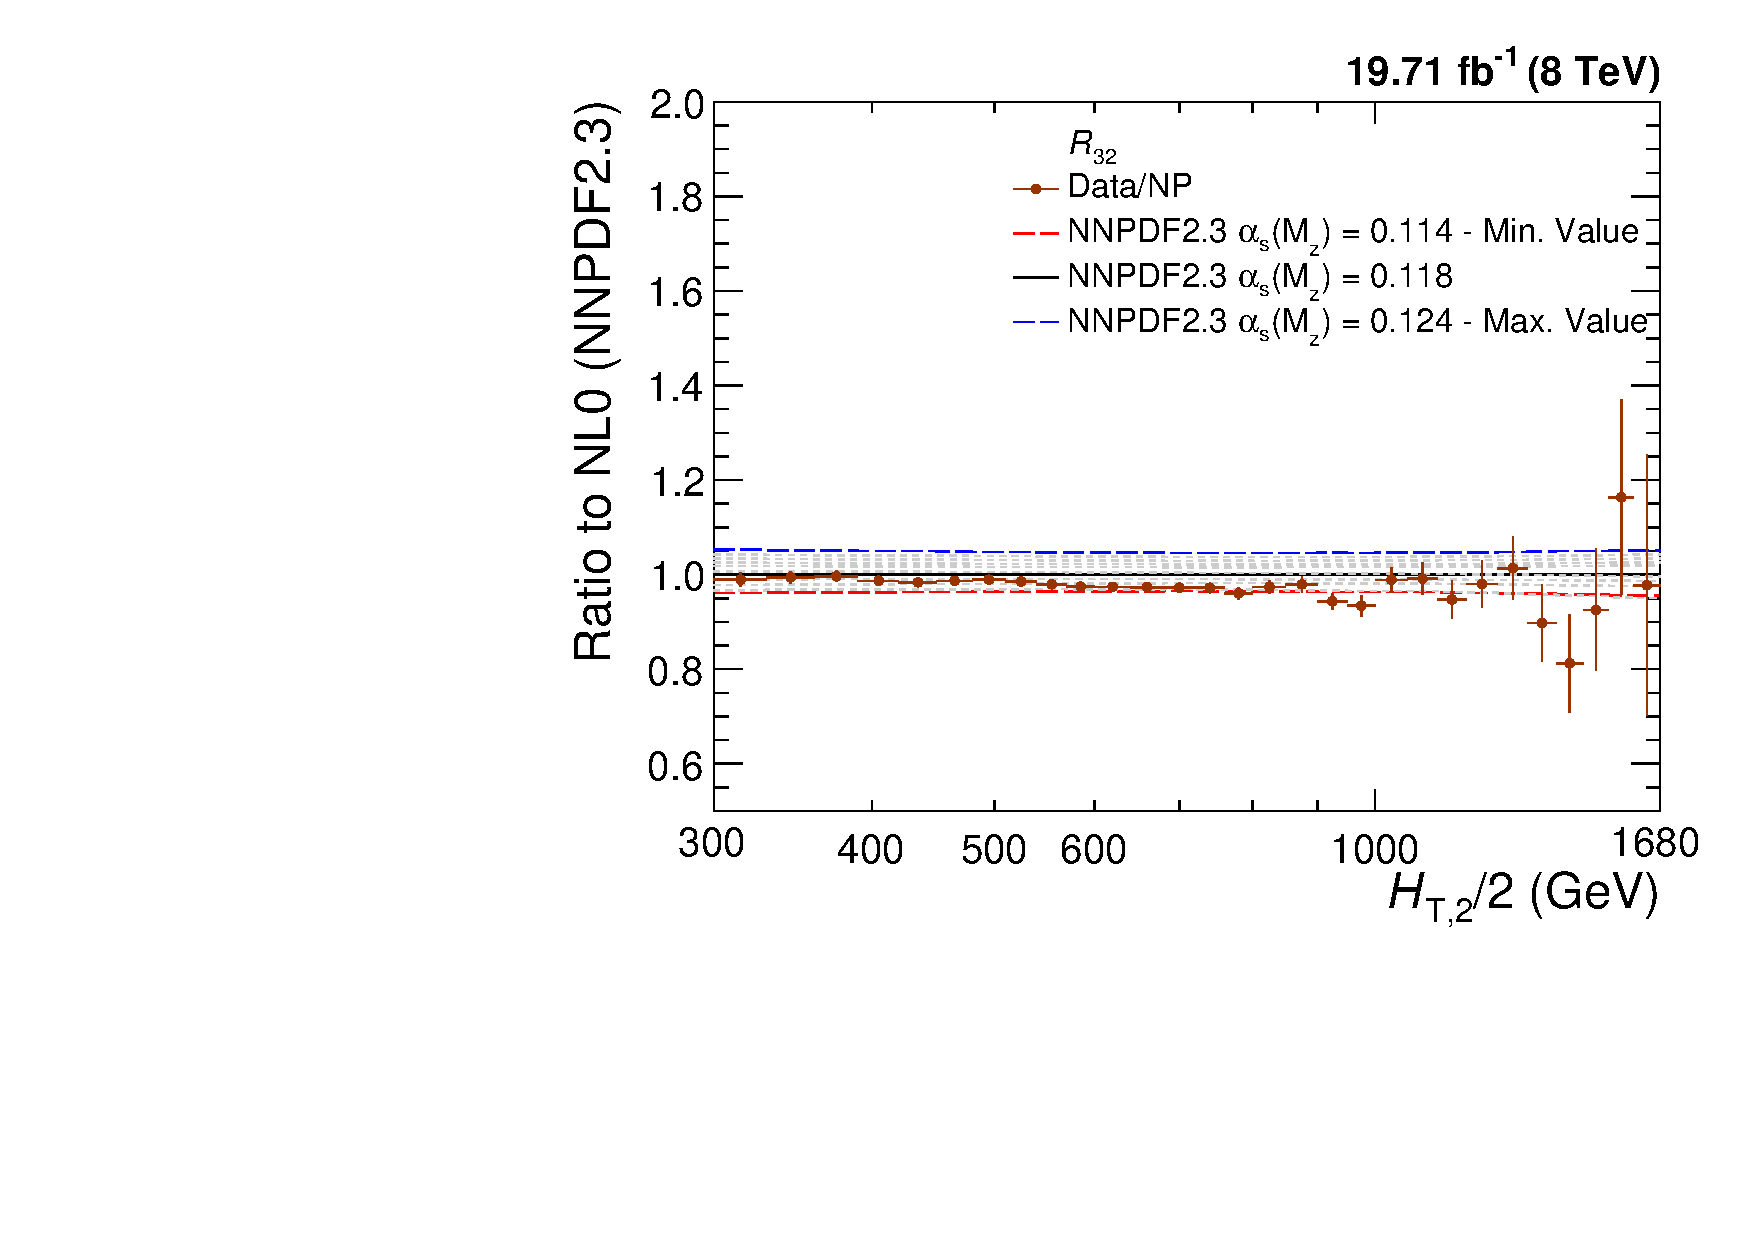
\includegraphics[width=0.51\textwidth]{Plots_HT_2_150/Sensitivity_double_ratio_32_NNPDF23.pdf}
 \caption{Ratio of the cross section ratio, \ratio to theory predictions using the CT10 (top left), the CT14 (top right), the MSTW2008 (middle left), the MMHT2014 (middle right) and NNPDF2.3 (bottom) NLO PDF sets for a series of values of \alpsmz. The \alpsmz value is varied in the range 0.112-0.127, 0.111-123, 0.110-0.130, 0.108-0.128 and 0.114-0.124 in steps of 0.001 for the CT10, CT14, MSTW2008, MMHT2014 and NNPDF2.3 NLO PDF sets, respectively. The error bars correspond to the total experimental uncertainty. The theory predictions are corrected for non-perturbative (NP) effects.}
 \label{fig:sensitivity_double_ratio}
 \end{center}
\end{figure}

\section{Determination of \texorpdfstring{\alpsmz}{alpha-S(M(Z))}}

As discussed in the previous section, the measured inclusive 2-jet and 3-jet event cross sections and their ratio \ratio can be used for a determination of the strong coupling constant \alpsmz. To extract the value of \alpsmz, a general fit procedure \cite{Chatrchyan:2013txa,Khachatryan:2014waa} has been followed and is described in the following section. 

\subsection{Fitting Procedure}
\label{sec:Fits}
The value of \alpsmz is determined by minimizing the chi-square (\chisq) between the experimental measurement and the theoretical predictions. The \chisq is defined as:

\begin{equation}
  \label{chisq}
  \chisq = M^{T}C^{-1}M\,,
\end{equation}
where $M$ is the vector of the differences between the data ($D^{i}$) and the theoretical values ($T^{i}$) in each bin $i$,

\begin{equation}
 \label{eqn:M_matrix}
 M^{i}=D^{i}-T^{i}
\end{equation}
and $C$ is the covariance matrix including all experimental uncertainties as described in Sec.~\ref{sec:exp_unc} and some theoretical uncertainties discussed in Sec.~\ref{sec:theory_unc}. The covariance matrix $C=C_\mathrm{exp}~\plus C_\mathrm{theo}$ is defined as the sum of covariances of experimental and theoretical sources of uncertainty as follows : 

\begin{eqnarray}
  \label{eqn:c_exp}
  C_\mathrm{exp} &=& \mathrm{Cov}^\mathrm{ExpStat}~\plus \sum\mathrm{Cov}^\mathrm{JEC}~\plus \mathrm{Cov}^\mathrm{Unfolding}~\plus \mathrm{Cov}^\mathrm{Lumi}~\plus \mathrm{Cov}^\mathrm{Residual}\,,\\
  C_\mathrm{theo} &=& \mathrm{Cov}^\mathrm{TheoStat}~\plus \mathrm{Cov}^\mathrm{NP}~\plus \mathrm{Cov}^\mathrm{PDF}\,,
  \label{eqn:c_theo}
\end{eqnarray}
where the labelled covariance matrices account for the following effects:

\begin{itemize}
\item{$\mathrm{Cov}^\mathrm{ExpStat}$: statistical uncertainty of the data including correlations introduced by the unfolding,}
\item{$\mathrm{Cov}^\mathrm{JEC}$: the JEC systematic uncertainty,}
\item{$\mathrm{Cov}^\mathrm{Unfolding}$: the unfolding systematic uncertainty including the JER,}
\item{$\mathrm{Cov}^\mathrm{Lumi}$: the luminosity uncertainty,}
\item{$\mathrm{Cov}^\mathrm{Residual}$: a residual uncorrelated systematic uncertainty summarizing individual causes such as small trigger and identification inefficiencies, time dependence of the jet \pt resolution, and uncertainty on the trigger prescale factors,}
\item{$\mathrm{Cov}^\mathrm{TheoStat}$: statistical uncertainty caused by numerical integrations in the cross section computations,}
\item{$\mathrm{Cov}^\mathrm{NP}$: the systematic uncertainty of the NP corrections, and}
\item{$\mathrm{Cov}^\mathrm{PDF}$: the PDF uncertainties.}
\end{itemize}

The Unfolding, JEC, Lumi and PDF and NP systematics are treated as 100$\%$ correlated among \httwo bins. If $\delta_i$ is the
total uncertainty on the double differential cross section, for the $i$-th \httwo bin, for any of these fully correlated sources, then the
$i,j$-th element of the corresponding covariance matrix is given by
\begin{equation*}
 COV_{ij} = \delta_i \times \delta_j
\end{equation*}

In fits of the ratio \ratio, the luminosity and residual uncorrelated
uncertainties cancel completely. Partial cancellations between the
other sources of uncertainty are taken into account in the fit.

The scale uncertainty is obtained by
varying the renormalization and factorization
scale by the six combinations of scale factors : ($\mu_F/\mu,\mu_R/\mu) = (0.5,0.5)$, $(2,2)$, $(1,0.5)$, $(1,2)$,
$(0.5,1)$, $(2,1)$, where $\mu=$ \httwo. The largest upwards and downwards deviations from the default factors are defined as the
scale uncertainty.

The treatment of PDF uncertainty depends on the individual PDF set. The PDF covariance matrix construction varies among different PDF sets. CT10 NLO PDF set has $N_{ev}=$26 eigen vectors with two PDF members viz. positive('+') and negative('-'). The PDF sets are denoted as $S_k^{\pm}$ for a given eigen vector $k$. Symmetric uncertainties due to PDF are then calculated using the formula \cite{CT10ERR}:

\begin{equation}
(\Delta X)^2 = \frac{1}{4} \sum_{k=1}^{N_{ev}} [X(S_k^{+}) - X(S_k^{-})]^2 \,,
\end{equation}

where $X(S_k^{\pm})$ are the double differential inclusive jet cross section for the $S_k^{\pm}$ PDF eigenvectors respectively.
The CT10 uncertainties are downscaled by a factor of 1.64 in order to have the uncertainties at the 68.3\% confidence level CL(1$\sigma$)
instead of 90\% CL(2$\sigma$).  
\begin{comment}
% The JES, unfolding, and luminosity uncertainties can be treated as
% multiplicative or additive.  When an uncertainty source is treated
% as multiplicative then $Cov_{i,j}=\sigma_i\sigma_j$ with $\sigma_i =
% \delta_{i} s^{Theory}_{i}$ where $\delta$ the uncertainty of each
% source and $s$ the cross section.  When an uncertainty source is
% treated as additive then $Cov_{i,j}=\sigma_i\sigma_j$ with $\sigma_i
% = \delta_{i} s^{Data}_{i}$.  The JES sources, the unfolding and
% luminosity uncertainties are multiplicative uncertainties and
% treated in this way.

The NNPDF2.3 PDF set comes with hundred different replicas ($N_{rep}$) instead of different eigenvectors, as for the previously discussed PDF sets. The mean uncertainty is calculated as average uncertainty from 100 different replicas. Following the prescription given in~\cite{NNPDFERR}, the PDF uncertainty is calculated as :

\begin{equation}
(\Delta X)^2 = \frac{1}{N_{rep}-1} \sum_{k=1}^{N_{rep}} [X(S_k) - \langle X(S_k) \rangle]^2 \,,
\end{equation}

where $\Delta X$ is the uncertainty on predicted double differential cross section, $X(S_k)$ is the double differential cross section for $k$-th replica and $\langle X \rangle$ is the average double differential cross section from all the replicas. 

The MSTW-2008 NLO PDF sets are also used to cross-check the \alpsmz extraction. The PDF uncertainties are derived in the same way as CT10, using 20 `+' and `-' eigenvectors.

First, fits to the cross sections are performed, where the range in
\httwo is restricted to be between 300\GeV and 1\TeV to avoid the
region close to the minimal \pt threshold of 150\GeV for each jet at
low \pt and the onset of electroweak effects at high \pt, which are
available for the dijet case only. The results are reported in
Table~\ref{tab:xsep300-1000} for the 2-jet and 3-jet event cross
sections and in Table~\ref{tab:xcomb300-1000} for a simultaneous fit
of both cross sections and for their ratio. In the ratio, EWK effects
are assumed to cancel as do the luminosity and the uncorrelated
uncertainty.

All cross section fits give compatible values for \alpsmz in the range
of 0.115--0.118; for the ratio \ratio somewhat smaller values are
obtained.  A common issue, except for the ratio fits, is the rather
small \chisqndof. A possible explanation is an overestimation of the
residual uncorrelated uncertainty of 1\% that is cancelled for \ratio.
If the fits are repeated with an assumed uncertainty of 0.25\%
instead, the \chisqndof values lie around unity while the \alpsmz
values are still compatible with the previous results but with
slightly reduced uncertainties.

%
% 300 - 1000 GeV
%
\begin{table}[htbp]
  \caption{Determination of \alpsmz from the inclusive 2-jet and
    3-jet event cross sections using five PDF sets at NLO\@. Only
    total uncertainties without scale variations are quoted.
    The results are obtained from a simultaneous fit to all 19 \httwo
    bins in the restricted range of $0.3 < \httwo < 1.0\TeV$.}
  \label{tab:xsep300-1000}
  \centering
  \begin{tabular}{lcccccc}
    \hline\hline
    \multirow{2}{*}{PDF set} & \multicolumn{3}{c}{2-jets} & \multicolumn{3}{c}{3-jets} \\
    & \alpsmz & $\pm\Delta\alpsmz$ & \chisqndof &\alpsmz & $\pm\Delta\alpsmz$ & \chisqndof \\\hline
    % v1 preapp
    % % ABM11          & 0.1240 & 0.0025 & 11./18 & 0.1241 & 0.0020 & 10./18 \\
    % CT10           & 0.1168 & 0.0033 & 2.6/18 & 0.1168 & 0.0027 & 5.6/18 \rbtrr\\
    % CT14           & 0.1157 & 0.0034 & 4.4/18 & 0.1155 & 0.0030 & 6.4/18 \rbtrr\\
    % MSTW2008       & 0.1150 & 0.0029 & 4.9/18 & 0.1162 & 0.0025 & 5.7/18 \rbtrr\\
    % MMHT2014       & 0.1154 & 0.0038 & 5.2/18 & 0.1161 & 0.0031 & 5.8/18 \rbtrr\\
    % NNPDF2.3       & 0.1156 & \color{Red}$^{+0.0033}_{-0.0026}$ & \color{Red}8.1/18 & 0.1163 & 0.0029 & 14./18 \rbtrr\\
    % v2
    % % ABM11          & 0.1304 & \color{Red}$^{+0.0011}_{-0.0024}$ & 29./18 & 0.1267 & 0.0016 & 17./18 \\
    % CT10           & 0.1169 & 0.0033 & 3.2/18 & 0.1169 & 0.0027 & 5.5/18 \rbtrr\\
    % CT14           & 0.1153 & 0.0036 & 5.7/18 & 0.1159 & 0.0031 & 6.2/18 \rbtrr\\
    % MSTW2008       & 0.1143 & 0.0027 & 8.9/18 & 0.1161 & 0.0021 & 6.8/18 \rbtrr\\
    % MMHT2014       & 0.1157 & 0.0034 & 10./18 & 0.1166 & 0.0025 & 7.1/18 \rbtrr\\
    % NNPDF2.3       & 0.1181 & 0.0025 & 14./18 & 0.1178 & 0.0021 & 9.1/18 \rbtrr\\
    % v2 2j ew
    % ABM11          & 0.1302 & \color{Red}$^{+0.0013}_{-0.0022}$ & 22./18 & 0.1267 & 0.0016 & 17./18 \\
    % CT10           & 0.1171 & 0.0032 & 3.1/18 & 0.1169 & 0.0027 & 5.5/18 \rbtrr\\
    % CT14           & 0.1158 & 0.0035 & 3.5/18 & 0.1159 & 0.0031 & 6.2/18 \rbtrr\\
    % MSTW2008       & 0.1158 & 0.0025 & 5.3/18 & 0.1161 & 0.0021 & 6.8/18 \rbtrr\\
    % MMHT2014       & 0.1163 & 0.0034 & 5.9/18 & 0.1166 & 0.0025 & 7.1/18 \rbtrr\\
    % NNPDF2.3       & 0.1182 & 0.0025 & 9.9/18 & 0.1178 & 0.0021 & 9.1/18 \rbtrr\\
    % v3 2j ew
    % ABM11          & 0.1302 & \color{Red}$^{+0.0013}_{-0.0022}$ & 22./18 & 0.1267 & 0.0016 & 17./18 \\
    CT10           & 0.1174 & 0.0032 & 3.0/18 & 0.1169 & 0.0027 & 5.4/18 \rbtrr\\
    CT14           & 0.1160 & 0.0035 & 3.5/18 & 0.1159 & 0.0031 & 6.1/18 \rbtrr\\
    MSTW2008       & 0.1159 & 0.0025 & 5.3/18 & 0.1161 & 0.0021 & 6.7/18 \rbtrr\\
    MMHT2014       & 0.1165 & 0.0034 & 5.9/18 & 0.1166 & 0.0025 & 7.1/18 \rbtrr\\
    NNPDF2.3       & 0.1183 & 0.0025 & 9.7/18 & 0.1179 & 0.0021 & 9.1/18 \rbtrr\\
    \hline\hline
  \end{tabular}
\end{table}

\begin{table}[htbp]
  \caption{Determination of \alpsmz from the inclusive 2-jet and
    3-jet event cross sections simultaneously and from their ratio
    \ratio using five PDF sets at NLO\@. Only
    total uncertainties without scale variations are quoted.
    The results are obtained from a simultaneous fit to all 38 (19) \httwo
    bins in the restricted range of $0.3 < \httwo < 1.0\TeV$.}
  \label{tab:xcomb300-1000}
  \centering
  \begin{tabular}{lcccccc}
    \hline\hline
    \multirow{2}{*}{PDF set} & \multicolumn{3}{c}{2- \& 3-jets} & \multicolumn{3}{c}{\ratio} \\
    & \alpsmz & $\pm\Delta\alpsmz$ & \chisqndof &\alpsmz & $\pm\Delta\alpsmz$ & \chisqndof \\\hline
    % v1 preapp
    % ABM11          & 0.1250 & 0.0018 & 19./37 & 0.1250 & 0.0024 & 23./18 \\
    % CT10           & 0.1167 & 0.0026 & 8.1/37 & \color{Red}0.1130 & \color{Red}$^{+0.0027}_{-0.0018}$ & \color{Red}14./18 \rbtrr\\
    % CT14           & 0.1159 & 0.0029 & 9.9/37 & 0.1140 & 0.0035 & 11./18 \rbtrr\\
    % MSTW2008       & 0.1156 & 0.0024 & 10./37 & 0.1161 & 0.0032 & 12./18 \rbtrr\\
    % MMHT2014       & 0.1161 & 0.0030 & 11./37 & 0.1162 & 0.0031 & 12./18 \rbtrr\\
    % NNPDF2.3       & 0.1169 & 0.0025 & 14./37 & 0.1181 & 0.0026 & 9.4/18 \rbtrr\\
    % v3 2j ew
    % ABM11          & 0.1278 & 0.0015 & 31./37 & 0.1233 & 0.0016 & 30./18 \\
    % CT10           & 0.1170 & 0.0026 & 8.2/37 & 0.1138 & 0.0027 & 15./18 \rbtrr\\
    % CT14           & 0.1161 & 0.0029 & 9.1/37 & 0.1137 & 0.0032 & 11./18 \rbtrr\\
    % MSTW2008       & 0.1161 & 0.0021 & 11./37 & 0.1149 & 0.0024 & 15./18 \rbtrr\\
    % MMHT2014       & 0.1168 & 0.0025 & 11./37 & 0.1143 & 0.0022 & 13./18 \rbtrr\\
    % NNPDF2.3       & 0.1188 & 0.0019 & 15./37 & 0.1181 & 0.0021 & 9.3/18 \rbtrr\\
    % v4 2j ew
    % ABM11          & 0.1278 & 0.0015 & 31./37 & 0.1238 & 0.0016 & 41./18 \\
    CT10           & 0.1170 & 0.0026 & 8.2/37 & 0.1141 & 0.0028 & 19./18 \rbtrr\\
    CT14           & 0.1161 & 0.0029 & 9.1/37 & 0.1139 & 0.0032 & 15./18 \rbtrr\\
    MSTW2008       & 0.1161 & 0.0021 & 11./37 & 0.1150 & 0.0023 & 21./18 \rbtrr\\
    MMHT2014       & 0.1168 & 0.0025 & 11./37 & 0.1142 & 0.0022 & 19./18 \rbtrr\\
    NNPDF2.3       & 0.1188 & 0.0019 & 15./37 & 0.1184 & 0.0021 & 12./18 \rbtrr\\
    \hline\hline
  \end{tabular}
\end{table}

To investigate how the EWK corrections affect the fit results for
\alpsmz, the range in \httwo is extended to $0.3 < \httwo < 1.68\TeV$.
Table~\ref{tab:xsep300-1680} reports the values obtained for \alpsmz
from fits to the 2-jet event cross section in this range with or
without EWK factors. The largest impact is a reduction in \chisqndof,
which indicates a better agreement when EWK effects are included. In
addition, a tendency to slightly smaller \alpsmz values is observed
without the EWK corrections. For the ratio \ratio it is expected that
these effects are much reduced.

%
% 300 - 1680 GeV, 2j only, w/o ew
%
\begin{table}[htbp]
  \caption{Determination of \alpsmz from the inclusive 2-jet
    event cross section using five PDF sets at NLO with (right) and
    without (left) EWK corrections. Only
    total uncertainties without scale variations are quoted.
    The results are obtained from a simultaneous fit to all 29 \httwo
    bins in the range of $0.3 < \httwo < 1.68\TeV$.}
  \label{tab:xsep300-1680}
  \centering
  \begin{tabular}{lcccccc}
    \hline\hline
    \multirow{2}{*}{PDF set} & \multicolumn{3}{c}{2-jets, no EWK} &
			    \multicolumn{3}{c}{2-jets, with EWK} \\
    & \alpsmz & $\pm\Delta\alpsmz$ & \chisqndof &\alpsmz & $\pm\Delta\alpsmz$ & \chisqndof \\\hline
    % v2                         v2 ew
    % % ABM11          & 0.1260 & 0.0019 & 50./28 & 0.1272 & 0.0018 & 39./28 \\
    % CT10           & 0.1157 & 0.0034 & 14./28 & 0.1160 & 0.0032 & 13./28 \rbtrr\\
    % CT14           & 0.1132 & 0.0031 & 22./28 & 0.1139 & 0.0031 & 15./28 \rbtrr\\
    % MSTW2008       & 0.1092 & \color{Red}$^{+0.0026}_{-0.0002}$ & 25./28 & 0.1131 & 0.0023 & 18./28 \rbtrr\\
    % MMHT2014       & 0.1124 & 0.0032 & 30./28 & 0.1137 & 0.0032 & 19./28 \rbtrr\\
    % NNPDF2.3       & 0.1159 & 0.0024 & 30./28 & 0.1165 & 0.0024 & 23./28 \rbtrr\\
    % v3                         v3 ew
    % ABM11          & 0.1262 & 0.0020 & 51./28 & 0.1273 & 0.0018 & 39./28 \\
    CT10           & 0.1163 & 0.0034 & 15./28 & 0.1165 & 0.0032 & 14./28 \rbtrr\\
    CT14           & 0.1137 & 0.0033 & 24./28 & 0.1144 & 0.0033 & 17./28 \rbtrr\\
    MSTW2008       & 0.1093 & 0.0028 & 27./28 & 0.1133 & 0.0023 & 19./28 \rbtrr\\
    MMHT2014       & 0.1127 & 0.0032 & 32./28 & 0.1141 & 0.0032 & 21./28 \rbtrr\\
    NNPDF2.3       & 0.1162 & 0.0024 & 31./28 & 0.1168 & 0.0024 & 23./28 \rbtrr\\
    \hline\hline
  \end{tabular}
\end{table}

From Figure~\ref{fig:R32_sensitivity} follows that only the PDF sets
MSTW2008 and MMHT2014 provide a large enough range in \alpsmz values
to ensure fits without extrapolation. The other three PDF sets are at
the limit such that reliable fits cannot be performed for all scale
settings and/or bins in scale
$Q=\httwo$. Tables~\ref{tab:xcomb300-1680}--\ref{tab:as_values_qbins}
give the complete results for MSTW2008 and MMHT2014 for the full range
in \httwo of 0.3\TeV up to 1.68\TeV, for scale variations in this
range, and for subranges in \httwo.

Using the MSTW PDF set, which dates from before the LHC start, the
strong coupling constant finally is determined to
%
\begin{eqnarray*}
  \alpsmz &=& 0.1150\,\pm0.0010\,\textrm{(exp)}\,\pm0.0013\,\textrm{(PDF)}\,\pm0.0015\,\textrm{(NP)}\,^{+0.0050}_{-0.0000}\,\textrm{(scale)}\\
  &=& 0.1150\,\pm0.0023\,\textrm{(all except scale)}\,^{+0.0050}_{-0.0000}\,\textrm{(scale)}\,.
\end{eqnarray*}
%
The MMHT PDF set, although using LHC jet data to determine the PDF
parameters, leads to a very similar result of
\begin{eqnarray*}
  \alpsmz &=& 0.1142\,\pm0.0010\,\textrm{(exp)}\,\pm0.0013\,\textrm{(PDF)}\,\pm0.0014\,\textrm{(NP)}\,^{+0.0049}_{-0.0006}\,\textrm{(scale)}\\
  &=& 0.1142\,\pm0.0022\,\textrm{(all except scale)}\,^{+0.0049}_{-0.0006}\,\textrm{(scale)}\,.
\end{eqnarray*}

%
% 300 - 1680 GeV, R_32 only, only MSTW/MMHT, pol2, asredrange
%
% Base fit
%
\begin{table}[p]
  \caption{Determination of \alpsmz from the ratio \ratio
    using the two most compatible PDF sets MSTW2008 and MMHT2014 at NLO\@.
    The results are obtained from a simultaneous fit to all 29 \httwo
    bins in the full range of $0.3 < \httwo < 1.68\TeV$.}
  \label{tab:xcomb300-1680}
  \centering
  \begin{tabular}{lccccccc}
    \hline\hline
    \multirow{2}{*}{PDF set} & & \multicolumn{5}{c}{\ratio: $\Delta\alpsmz\cdot1000$} & \\
    & \alpsmz & exp. & PDF & NP & all exc.\ scale & scale & \chisqndof \rbthm\\\hline
    % v1 preapp
    % MSTW2008       & 0.1149 & $\pm10$ & $\pm29$ & $\pm32$ & $^{+45}_{-0}$ & 16./28 \rbtrr\\
    % MMHT2014       & 0.1143 & $\pm10$ & $\pm29$ & $\pm31$ & $^{+47}_{-0}$ & 14./28 \rbtrr\\
    % v3
    % MSTW2008       & 0.1149 & $\pm11$ & & $\pm15$ $\pm15$ & $\pm24$ & $^{+50}_{-0}$ & 16./28 \rbtrr\\
    % MMHT2014       & 0.1143 & $\pm11$ & & $\pm11$ $\pm15$ & $\pm22$ & $^{+48}_{-2}$ & 14./28 \rbtrr\\
    % v4
    MSTW2008       & 0.1150 & $\pm10$ & $\pm13$ & $\pm15$ & $\pm23$ & $^{+50}_{-0}$ & 26./28 \rbtrr\\
    MMHT2014       & 0.1142 & $\pm10$ & $\pm13$ & $\pm14$ & $\pm22$ & $^{+49}_{-6}$ & 24./28 \rbtrr\\
    \hline\hline
  \end{tabular}
\end{table}
%
% Scale variations
%
\begin{table}[htbp]
  \caption{Fitted values of \alpsmz using \ratio in the \httwo range from 0.3 up
    to 1.68\TeV at the central scale and for the six scale factor
    combinations for the two PDF sets MSTW2008 and MMHT2014.}
  \label{tab:as_values_scalevar}
  \centering
  \begin{tabular}{cccccc}
    \hline\hline
    \multirow{2}{*}{$\mur/\httwo$} & \multirow{2}{*}{$\muf/\httwo$} &
    \multicolumn{2}{c}{MSTW2008} & \multicolumn{2}{c}{MMHT2014}\rbtrr\\
    & & \alpsmz & \chisqndof & \alpsmz & \chisqndof\rbthm\\\hline
    % v1 preapp
    % $1$    & $1$    & $0.1159$ & $14./28$ & $0.1160$ & $14./28$\rbtrr\\
    % $1/2$  & $1/2$  & $0.1212$ & $30./28$ & $0.1209$ & $31./28$\rbtrr\\
    % $2$    & $2$    & $0.1200$ & $11./28$ & $0.1197$ & $12./28$\rbtrr\\
    % $1/2$  & $1$    & $0.1182$ & $21./28$ & $0.1175$ & $21./28$\rbtrr\\
    % $1$    & $1/2$  & $0.1169$ & $15./28$ & $0.1165$ & $15./28$\rbtrr\\
    % $1$    & $2$    & $0.1169$ & $13./28$ & $0.1164$ & $13./28$\rbtrr\\
    % $2$    & $1$    & $0.1187$ & $12./28$ & $0.1184$ & $12./28$\rbtrr\\
    % v3
    % $1$    & $1$    & $0.1149$ & $16./28$ & $0.1143$ & $14./28$\rbtrr\\
    % $1/2$  & $1/2$  & $0.1176$ & $52./28$ & $0.1169$ & $50./28$\rbtrr\\
    % $2$    & $2$    & $0.1198$ & $9.7/28$ & $0.1191$ & $10./28$\rbtrr\\
    % $1/2$  & $1$    & $0.1152$ & $35./28$ & $0.1141$ & $32./28$\rbtrr\\
    % $1$    & $1/2$  & $0.1149$ & $19./28$ & $0.1143$ & $17./28$\rbtrr\\
    % $1$    & $2$    & $0.1153$ & $14./28$ & $0.1148$ & $13./28$\rbtrr\\
    % $2$    & $1$    & $0.1178$ & $11./28$ & $0.1175$ & $11./28$\rbtrr\\
    % v3
    $1$    & $1$    & $0.1150$ & $26./28$ & $0.1142$ & $24./28$\rbtrr\\
    $1/2$  & $1/2$  & $0.1165$ & $77./28$ & $0.1160$ & $73./28$\rbtrr\\
    $2$    & $2$    & $0.1120$ & $18./28$ & $0.1191$ & $18./28$\rbtrr\\
    $1/2$  & $1$    & $0.1150$ & $53./28$ & $0.1136$ & $48./28$\rbtrr\\
    $1$    & $1/2$  & $0.1150$ & $30./28$ & $0.1142$ & $28./28$\rbtrr\\
    $1$    & $2$    & $0.1155$ & $23./28$ & $0.1147$ & $22./28$\rbtrr\\
    $2$    & $1$    & $0.1180$ & $19./28$ & $0.1175$ & $19./28$\rbtrr\\
    \hline\hline
  \end{tabular}
\end{table}
%
% Q bins
%
\begin{table}[htbp]
  \caption{Uncertainty composition for \alpsmz from the determination
    of \alps from the jet event rate \ratio in bins of \httwo.
    The statistical uncertainty of the NLO computation is negligible
    in comparison to any of the other sources of uncertainty.
    Electroweak corrections, significant only at high \httwo,
    are assumed to cancel between the numerator and denominator.}
  \label{tab:as_values_qbins}
  \centering
  \begin{tabular}{ccccccccccc}
    \hline\hline
    \httwo & % $\langle{}Q\rangle$ &
    \multicolumn{5}{c}{MSTW2008: $\Delta\alpsmz\cdot1000$} &
    \multicolumn{5}{c}{MMHT2014: $\Delta\alpsmz\cdot1000$} \\
    (\GeV) & % (\GeV) &
    \alpsmz & exp. & PDF & NP & scale &
    \alpsmz & exp. & PDF & NP & scale \rbthm\\\hline
    % v1 preapp
    % 300--420 \rbtrr  & %474 &
    % 0.1169 & $\pm{15}$ & $\pm{27}$      & $^{+73}_{-18}$ &
    % 0.1170 & $\pm{15}$ & $\pm{25}$      & $^{+73}_{-17}$\\
    % 420--600 \rbtrr  & %664 &
    % 0.1158 & $\pm{11}$ & $\pm{31}$      & $^{+54}_{-12}$ &
    % 0.1161 & $\pm{11}$ & $\pm{31}$      & $^{+57}_{-9}$\\
    % 600--1000\rbtrr  & %896 &
    % 0.1143 & $\pm{13}$ & $\pm{31}$      & $^{+52}_{-10}$ &
    % 0.1148 & $\pm{12}$ & $\pm{29}$      & $^{+49}_{-10}$\\
    % 1000--1680\rbtrr & %896 &
    % 0.1168 & $\pm{33}$ & $^{+26}_{-56}$ & $^{+42}_{-6}$ &
    % 0.1171 & $\pm{30}$ & $^{+25}_{-48}$ & $^{+44}_{-6}$\\\hline
    % 300--1680\rbtrr  & %896 &
    % 0.1159 & $\pm{10}$ & $\pm{29}$      & $^{+46}_{-9}$ &
    % 0.1160 & $\pm{10}$ & $\pm{29}$      & $^{+47}_{-4}$\\
    % v3
    % 300--420 \rbtrr  & %474 &
    % 0.1157 & $\pm{15}$ & $\pm{13}$    & $\pm{20}$     & $^{+53}_{-0}$ &
    % 0.1159 & $\pm{15}$ & $\pm{12}$    & $\pm{19}$     & $^{+51}_{-0}$\\
    % 420--600 \rbtrr  & %664 &
    % 0.1153 & $\pm{12}$ & $\pm{14}$    & $\pm{18}$     & $^{+57}_{-0}$ &
    % 0.1155 & $\pm{11}$ & $\pm{12}$    & $\pm{17}$     & $^{+55}_{-0}$\\
    % 600--1000\rbtrr  & %896 &
    % 0.1135 & $\pm{14}$ & $\pm{14}$    & $\pm{19}$     & $^{+55}_{-0}$ &
    % 0.1141 & $\pm{13}$ & $\pm{12}$    & $\pm{18}$     & $^{+48}_{-0}$\\
    % 1000--1680\rbtrr & %896 &
    % 0.1147 & $\pm{38}$ & $\pm{16}$    & $\pm{18}$     & $^{+63}_{-11}$ &
    % 0.1154 & $\pm{34}$ & $\pm{13}$    & $\pm{17}$     & $^{+56}_{-10}$\\\hline
    % 300--1680\rbtrr  & %896 &
    % 0.1149 & $\pm{11}$ & $\pm{15}$    & $\pm{15}$     & $^{+50}_{-0}$ &
    % 0.1143 & $\pm{11}$ & $\pm{11}$    & $\pm{15}$     & $^{+48}_{-2}$\\
    % v4
    300--420 \rbtrr  & %474 &
    0.1157 & $\pm{15}$ & $\pm{14}$    & $\pm{19}$     & $^{+53}_{-0}$ &
    0.1158 & $\pm{14}$ & $\pm{10}$    & $\pm{19}$     & $^{+52}_{-0}$\\
    420--600 \rbtrr  & %664 &
    0.1153 & $\pm{11}$ & $\pm{14}$    & $\pm{18}$     & $^{+57}_{-0}$ &
    0.1154 & $\pm{11}$ & $\pm{12}$    & $\pm{17}$     & $^{+56}_{-0}$\\
    600--1000\rbtrr  & %896 &
    0.1134 & $\pm{13}$ & $\pm{16}$    & $\pm{19}$     & $^{+52}_{-0}$ &
    0.1140 & $\pm{12}$ & $\pm{12}$    & $\pm{18}$     & $^{+45}_{-0}$\\
    1000--1680\rbtrr & %896 &
    0.1147 & $\pm{29}$ & $\pm{17}$    & $\pm{18}$     & $^{+63}_{-11}$ &
    0.1154 & $\pm{25}$ & $\pm{14}$    & $\pm{15}$     & $^{+56}_{-11}$\\\hline
    300--1680\rbtrr  & %896 &
    0.1150 & $\pm{10}$ & $\pm{13}$    & $\pm{15}$     & $^{+50}_{-0}$ &
    0.1142 & $\pm{10}$ & $\pm{13}$    & $\pm{14}$     & $^{+49}_{-6}$\\
    \hline\hline
  \end{tabular}
\end{table}
%\begin{figure}[!htbp]
%\begin{center}
%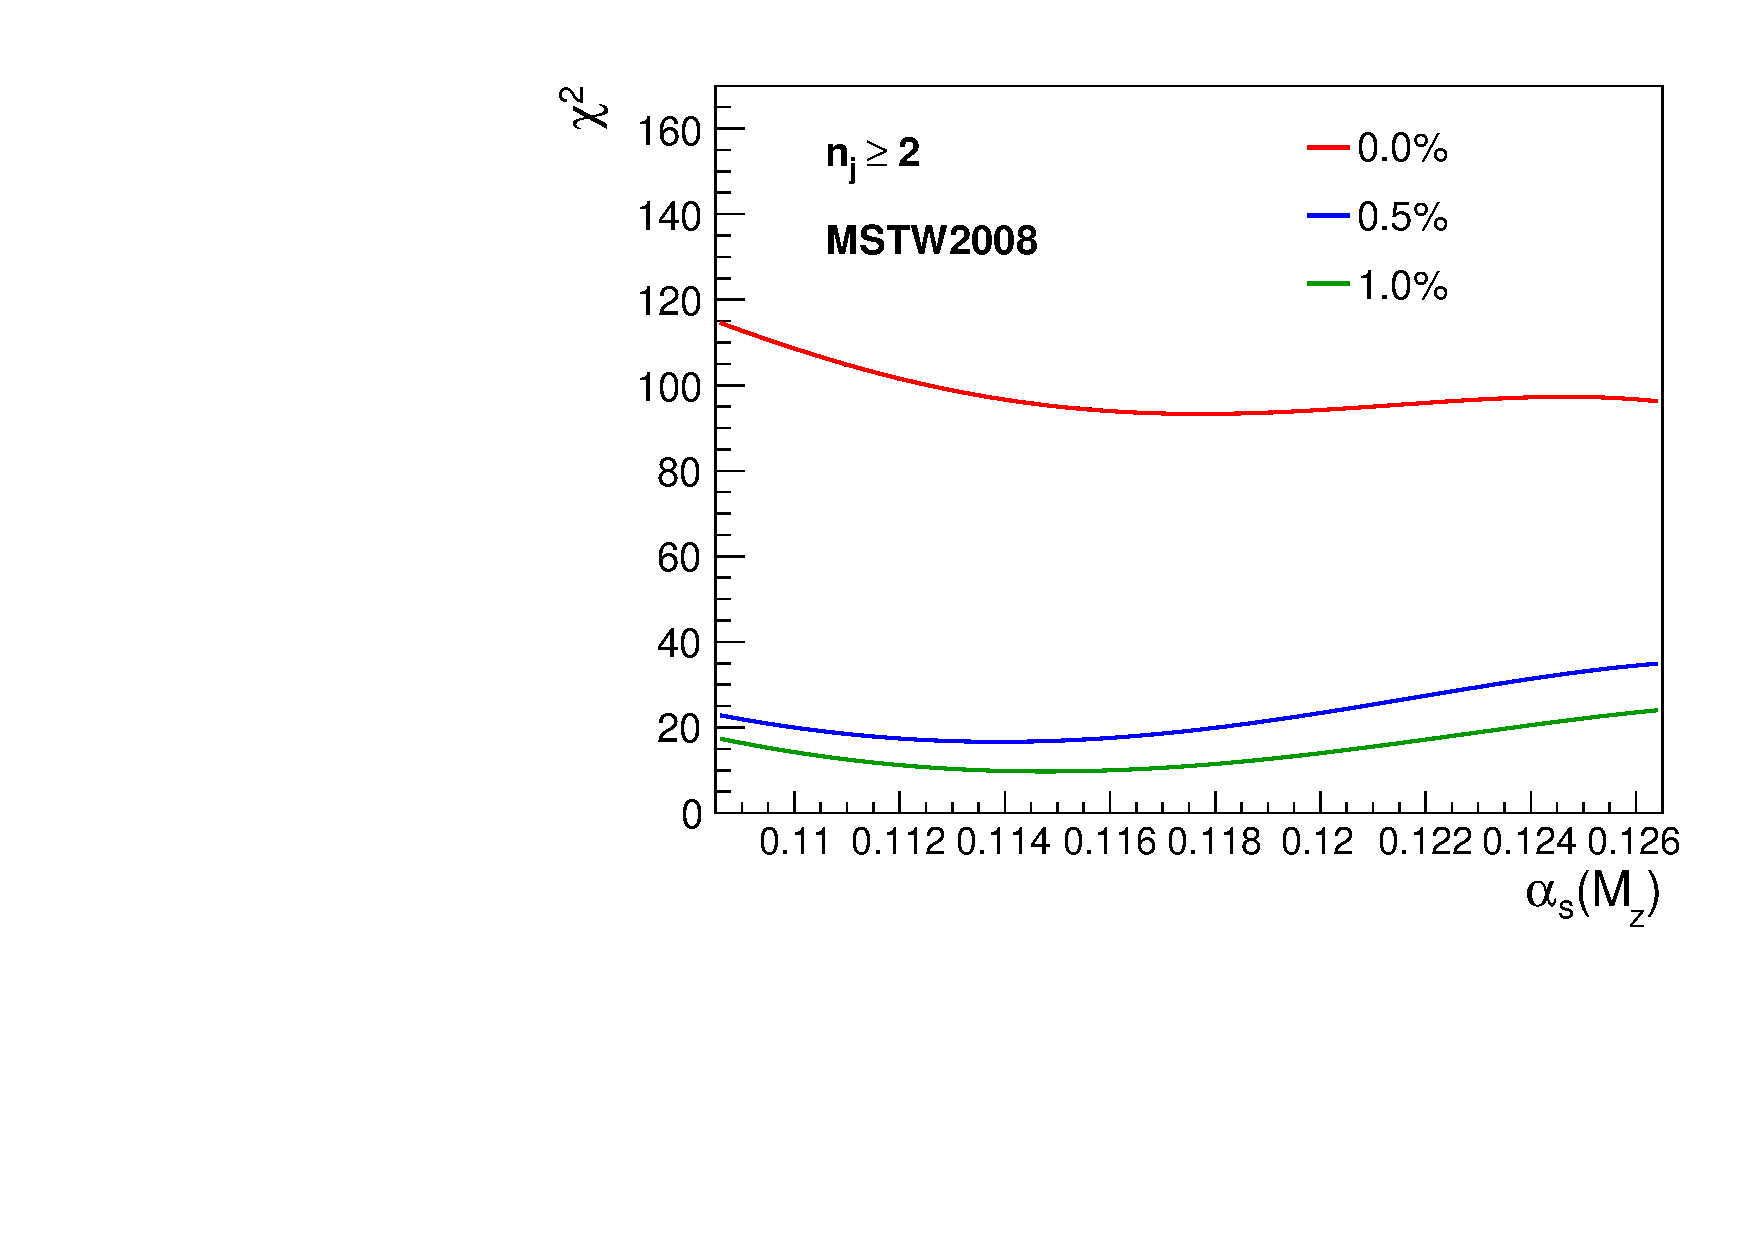
\includegraphics[width=0.5\textwidth]{Plots_HT_2_150/Fits/OutputPlot_2j_mstw.pdf}%
%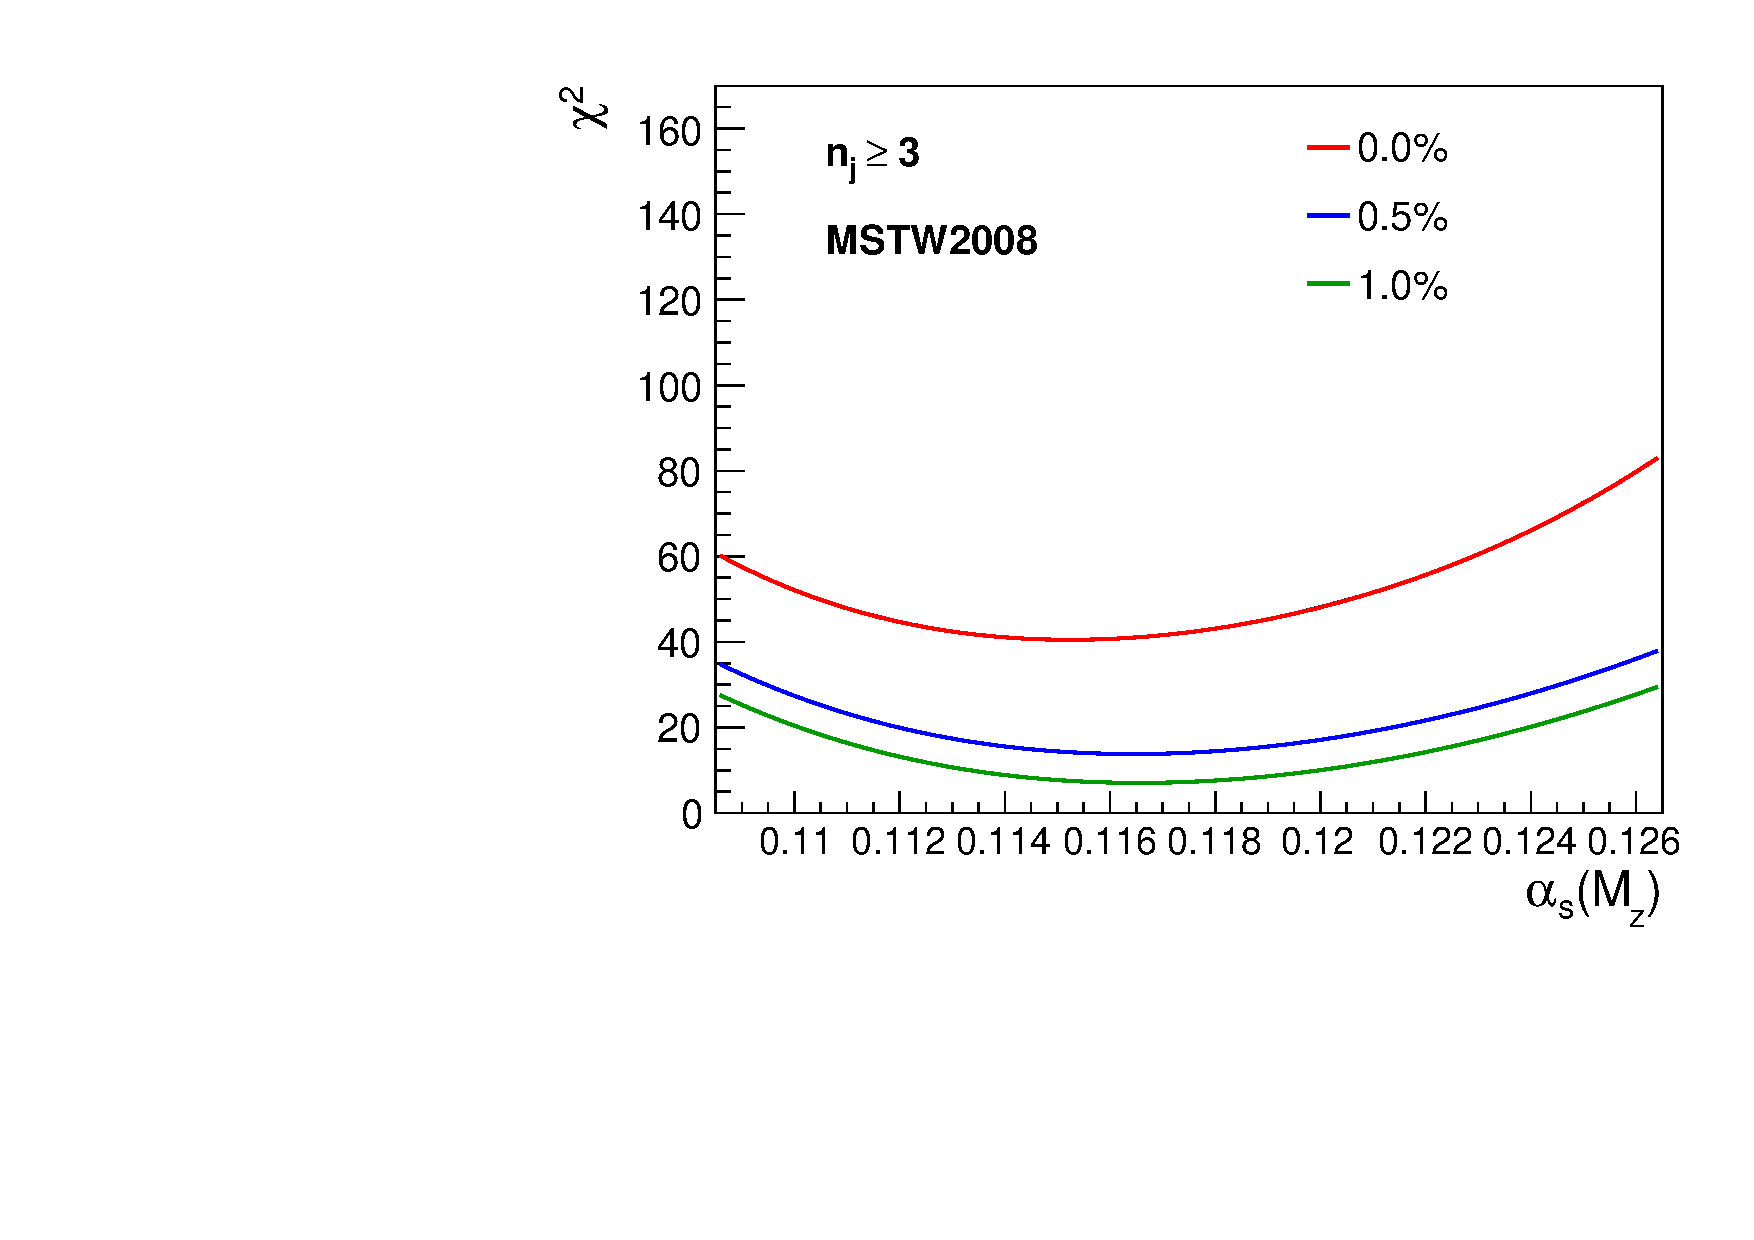
\includegraphics[width=0.5\textwidth]{Plots_HT_2_150/Fits/OutputPlot_3j_mstw.pdf}\\
%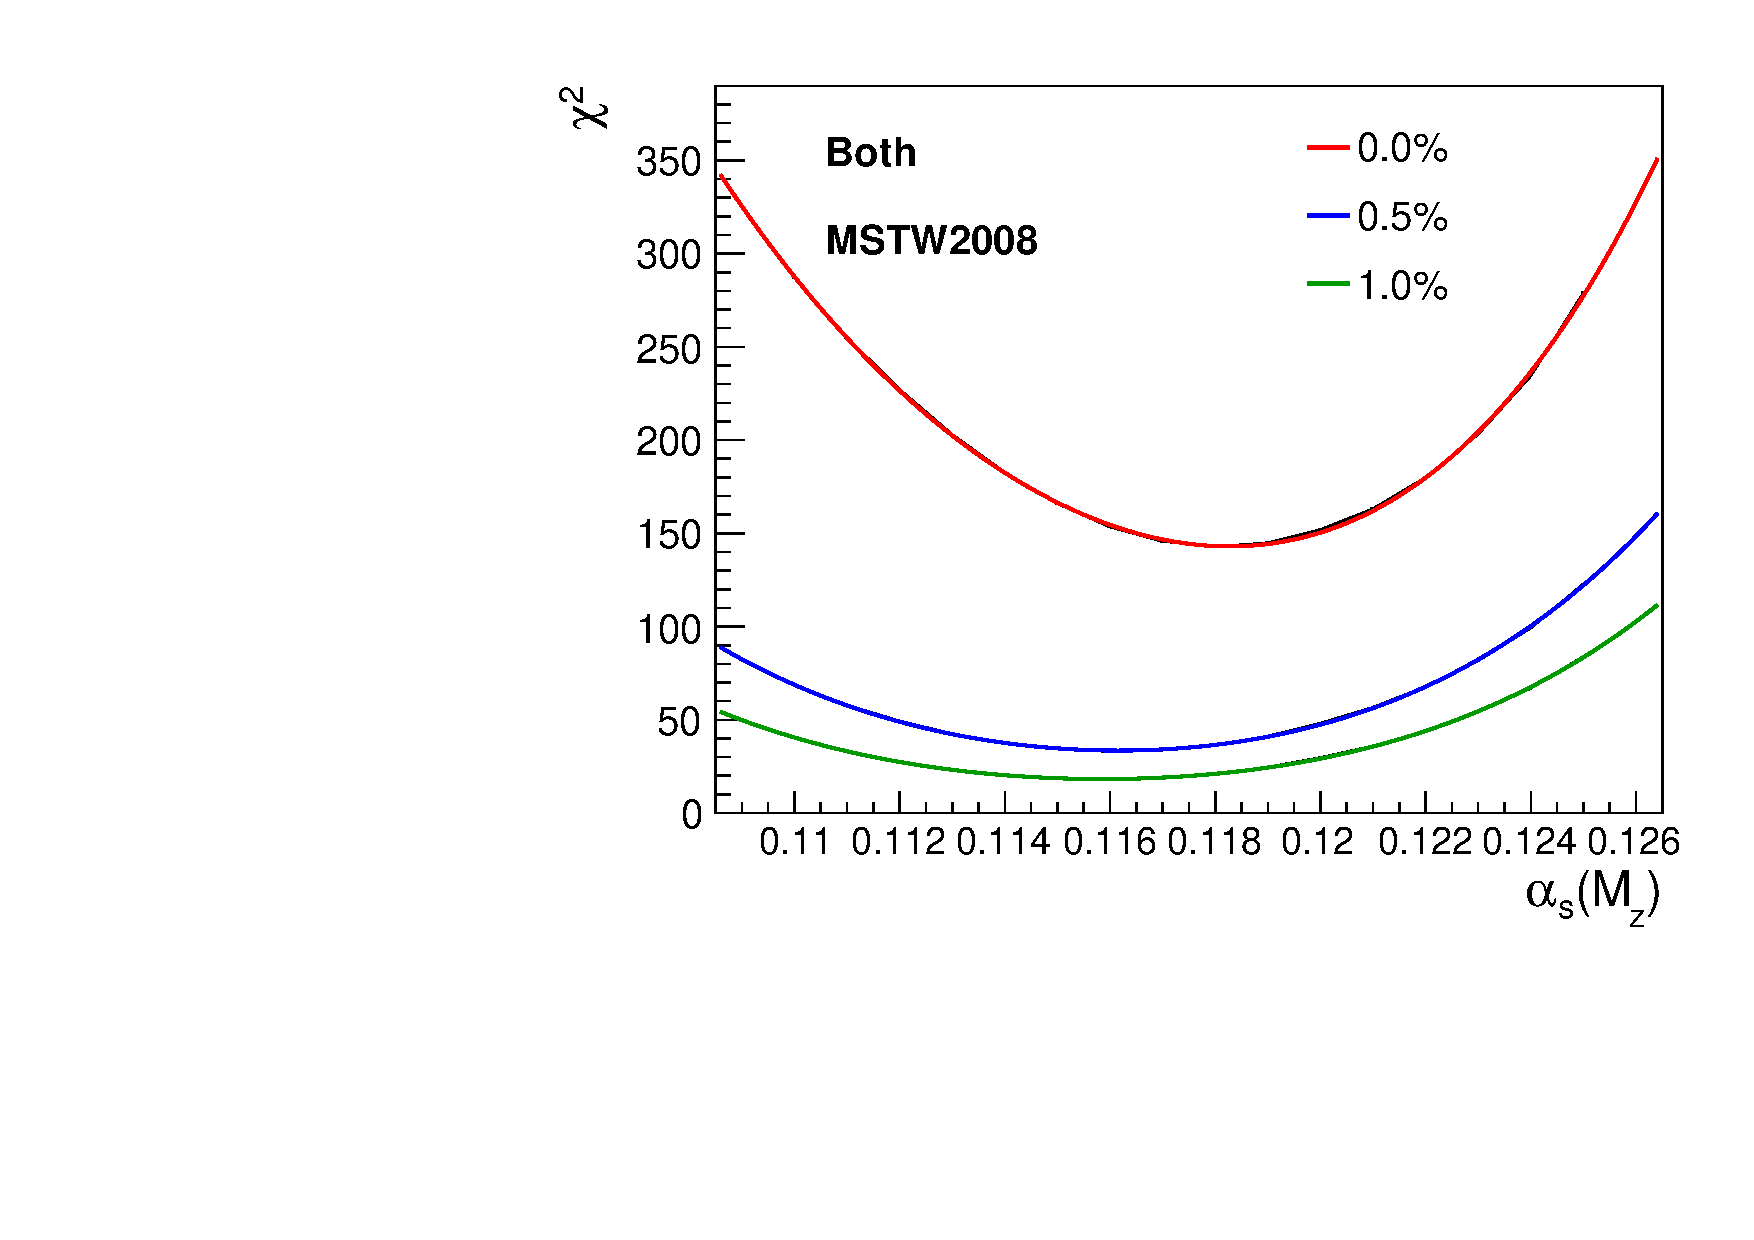
\includegraphics[width=0.5\textwidth]{Plots_HT_2_150/Fits/OutputPlot_nj_mstw.pdf}%
%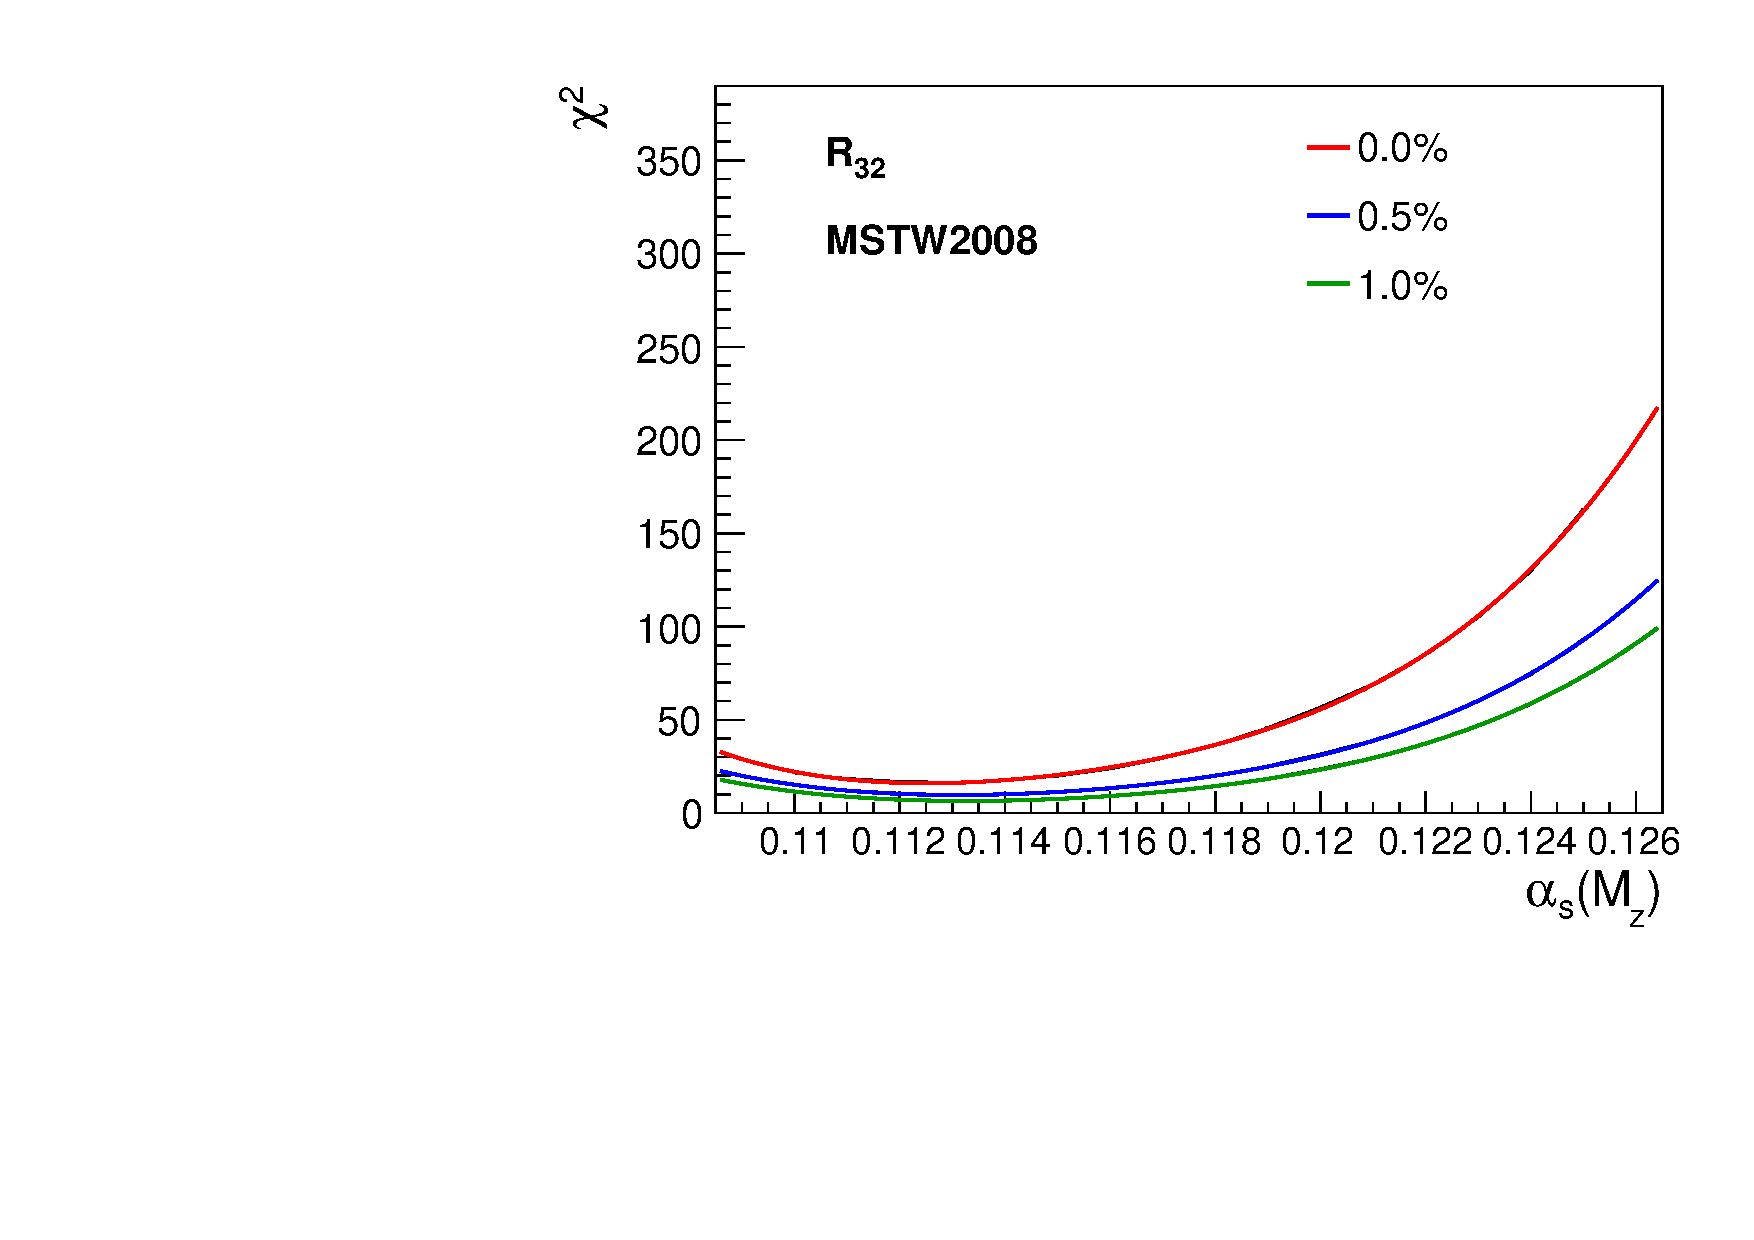
\includegraphics[width=0.5\textwidth]{Plots_HT_2_150/Fits/OutputPlot_r32_mstw.pdf}\\
%\caption{Variation of Uncorrelated Uncertainty.}
%\label{fig:unc_variation}
%\end{center}
%\end{figure}
%
%\begin{figure}[!htbp]
%\begin{center}
%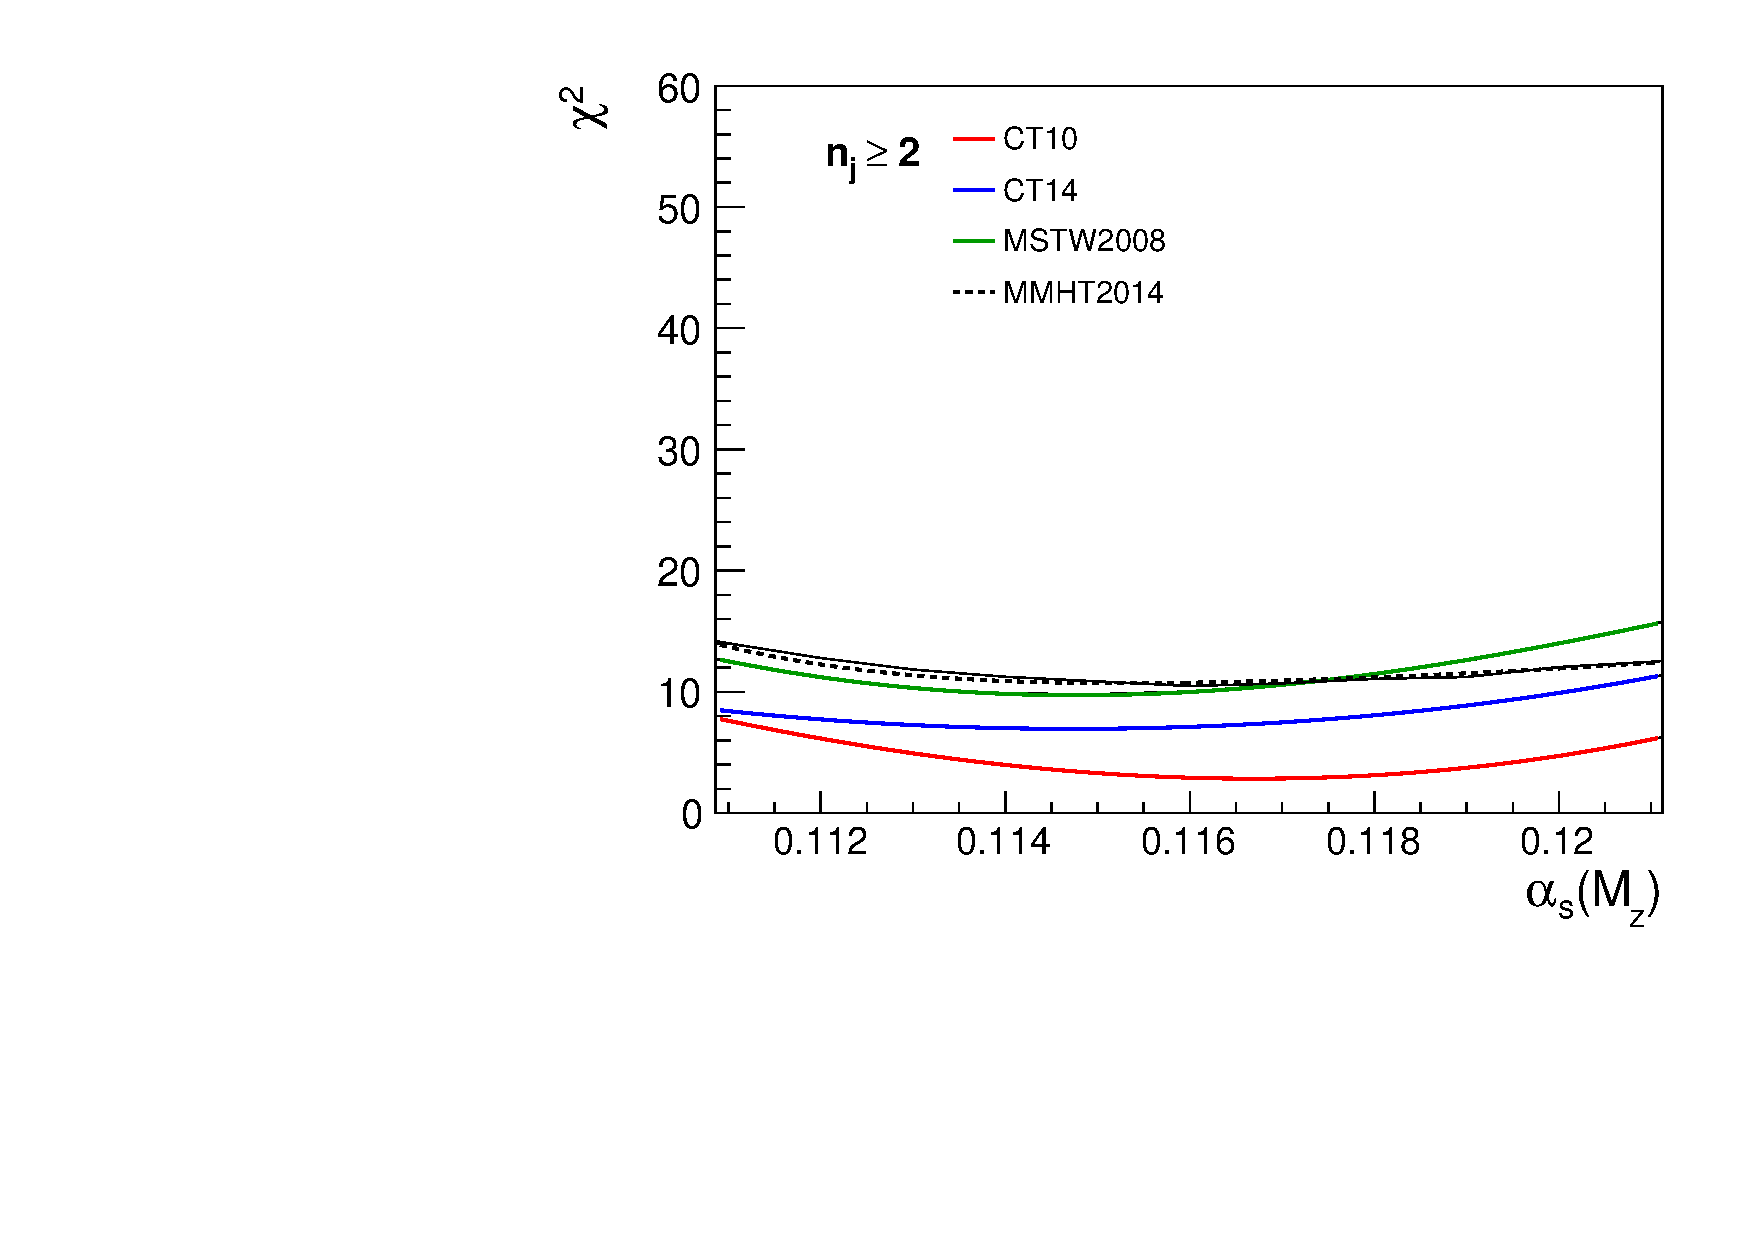
\includegraphics[width=0.5\textwidth]{Plots_HT_2_150/Fits/OutputPlot_2j_100.pdf}%
%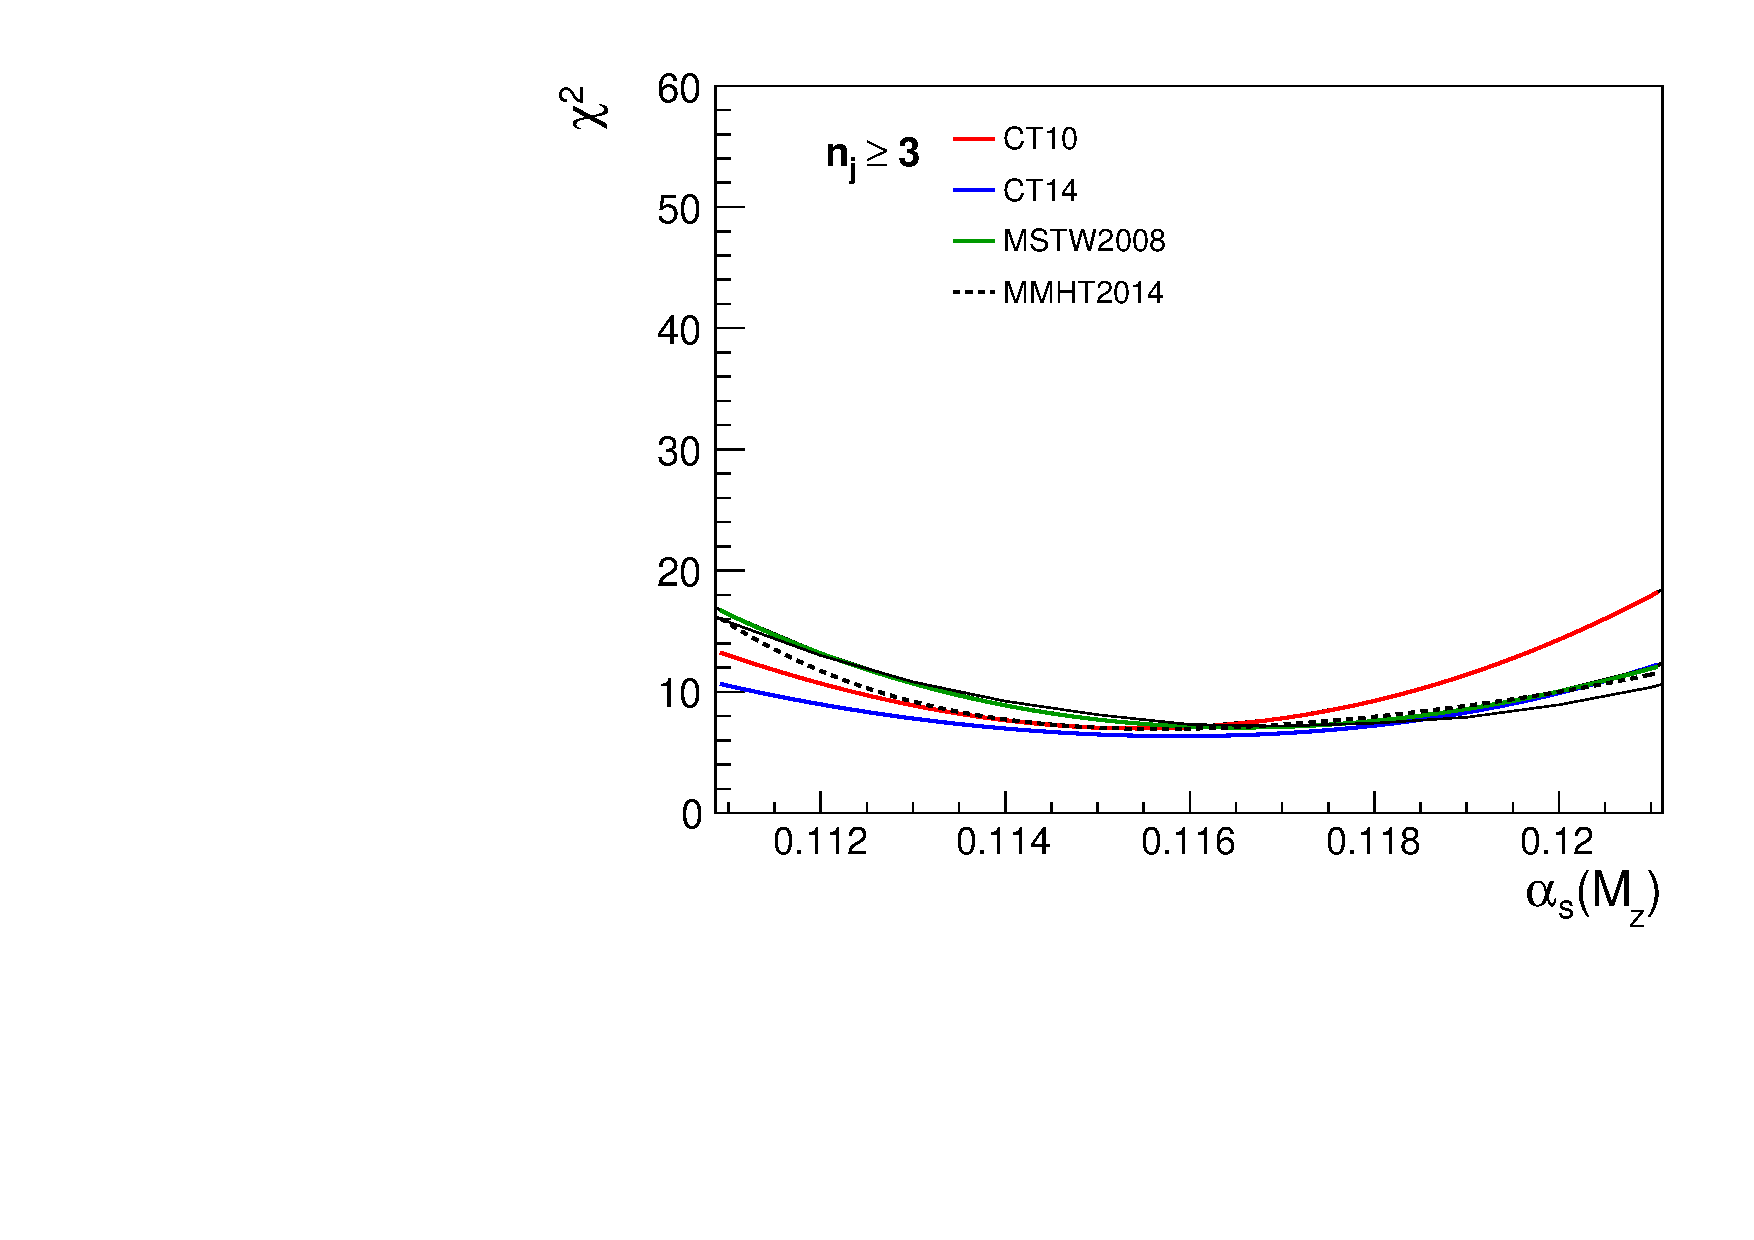
\includegraphics[width=0.5\textwidth]{Plots_HT_2_150/Fits/OutputPlot_3j_100.pdf}\\
%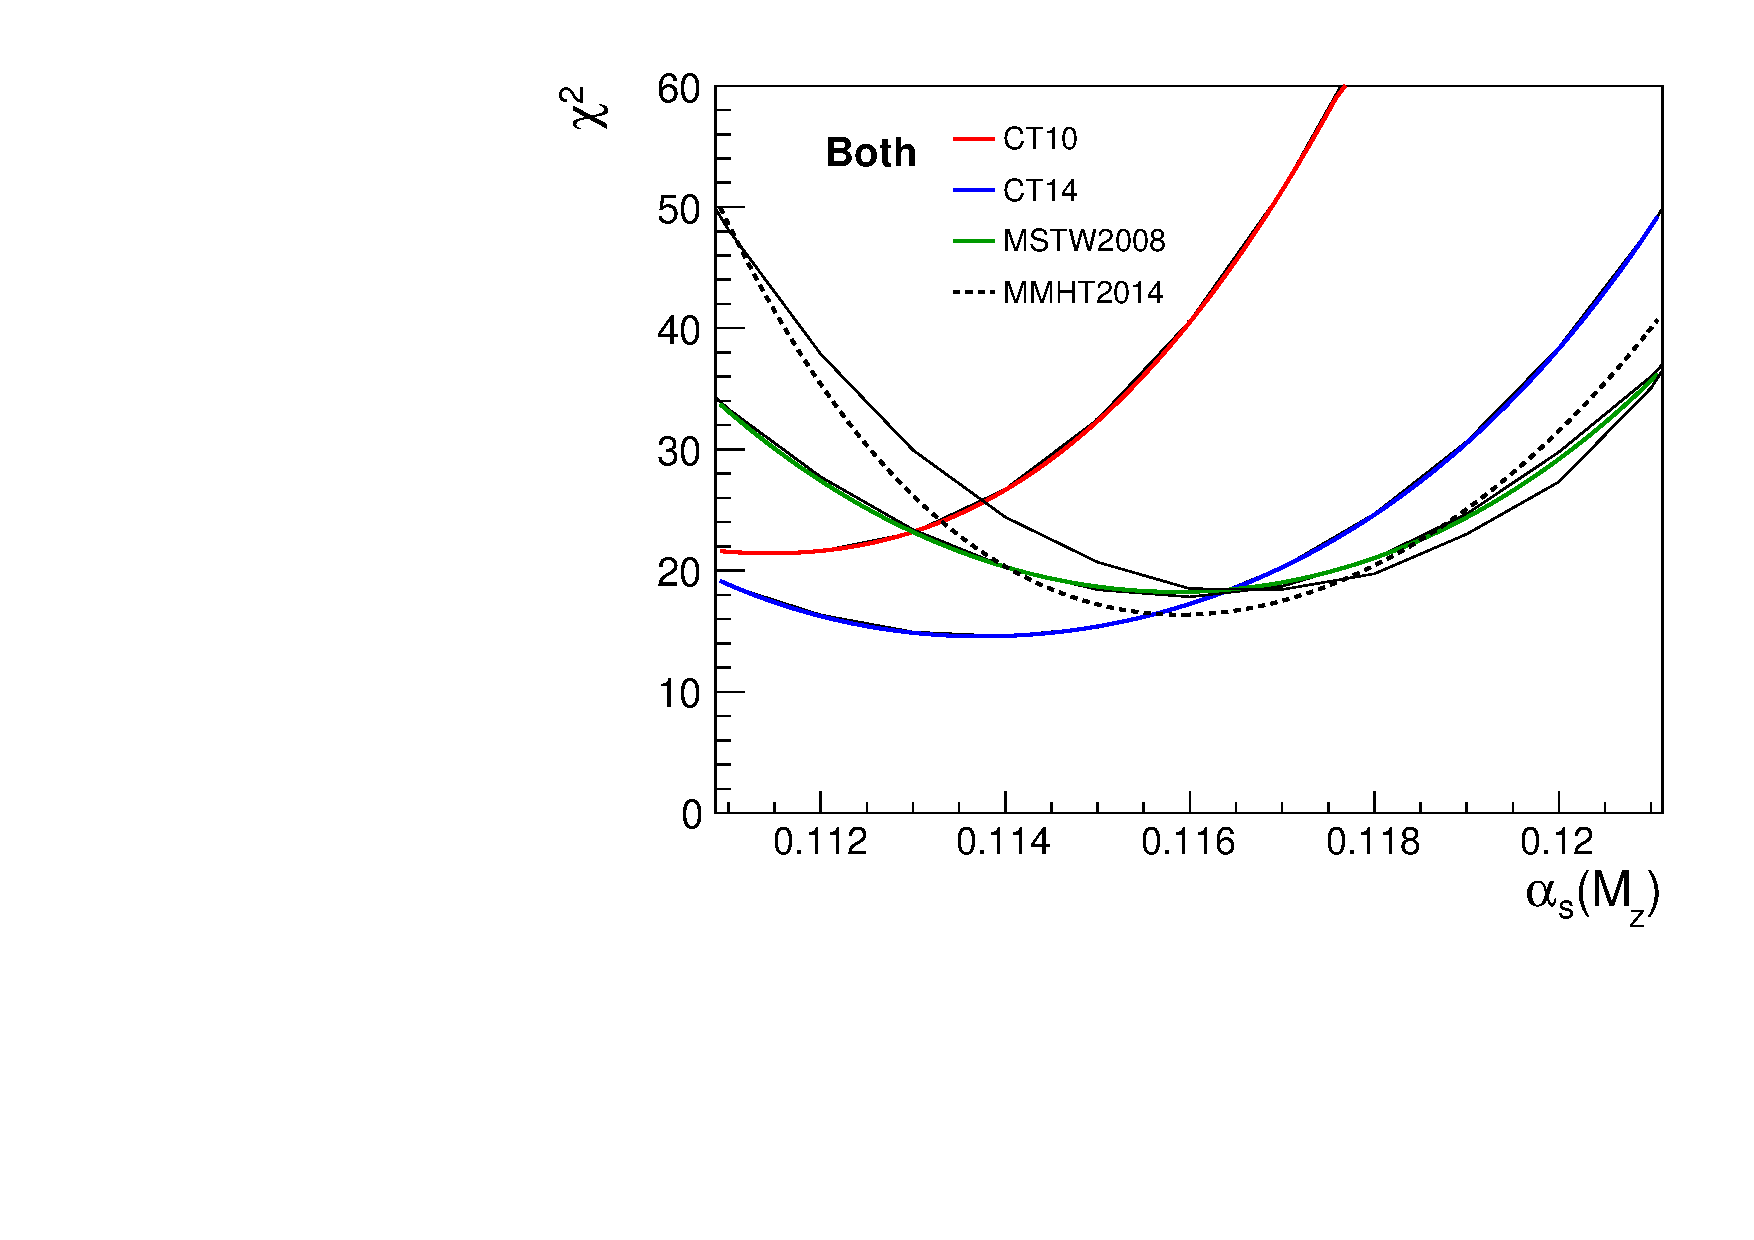
\includegraphics[width=0.5\textwidth]{Plots_HT_2_150/Fits/OutputPlot_nj_100.pdf}%
%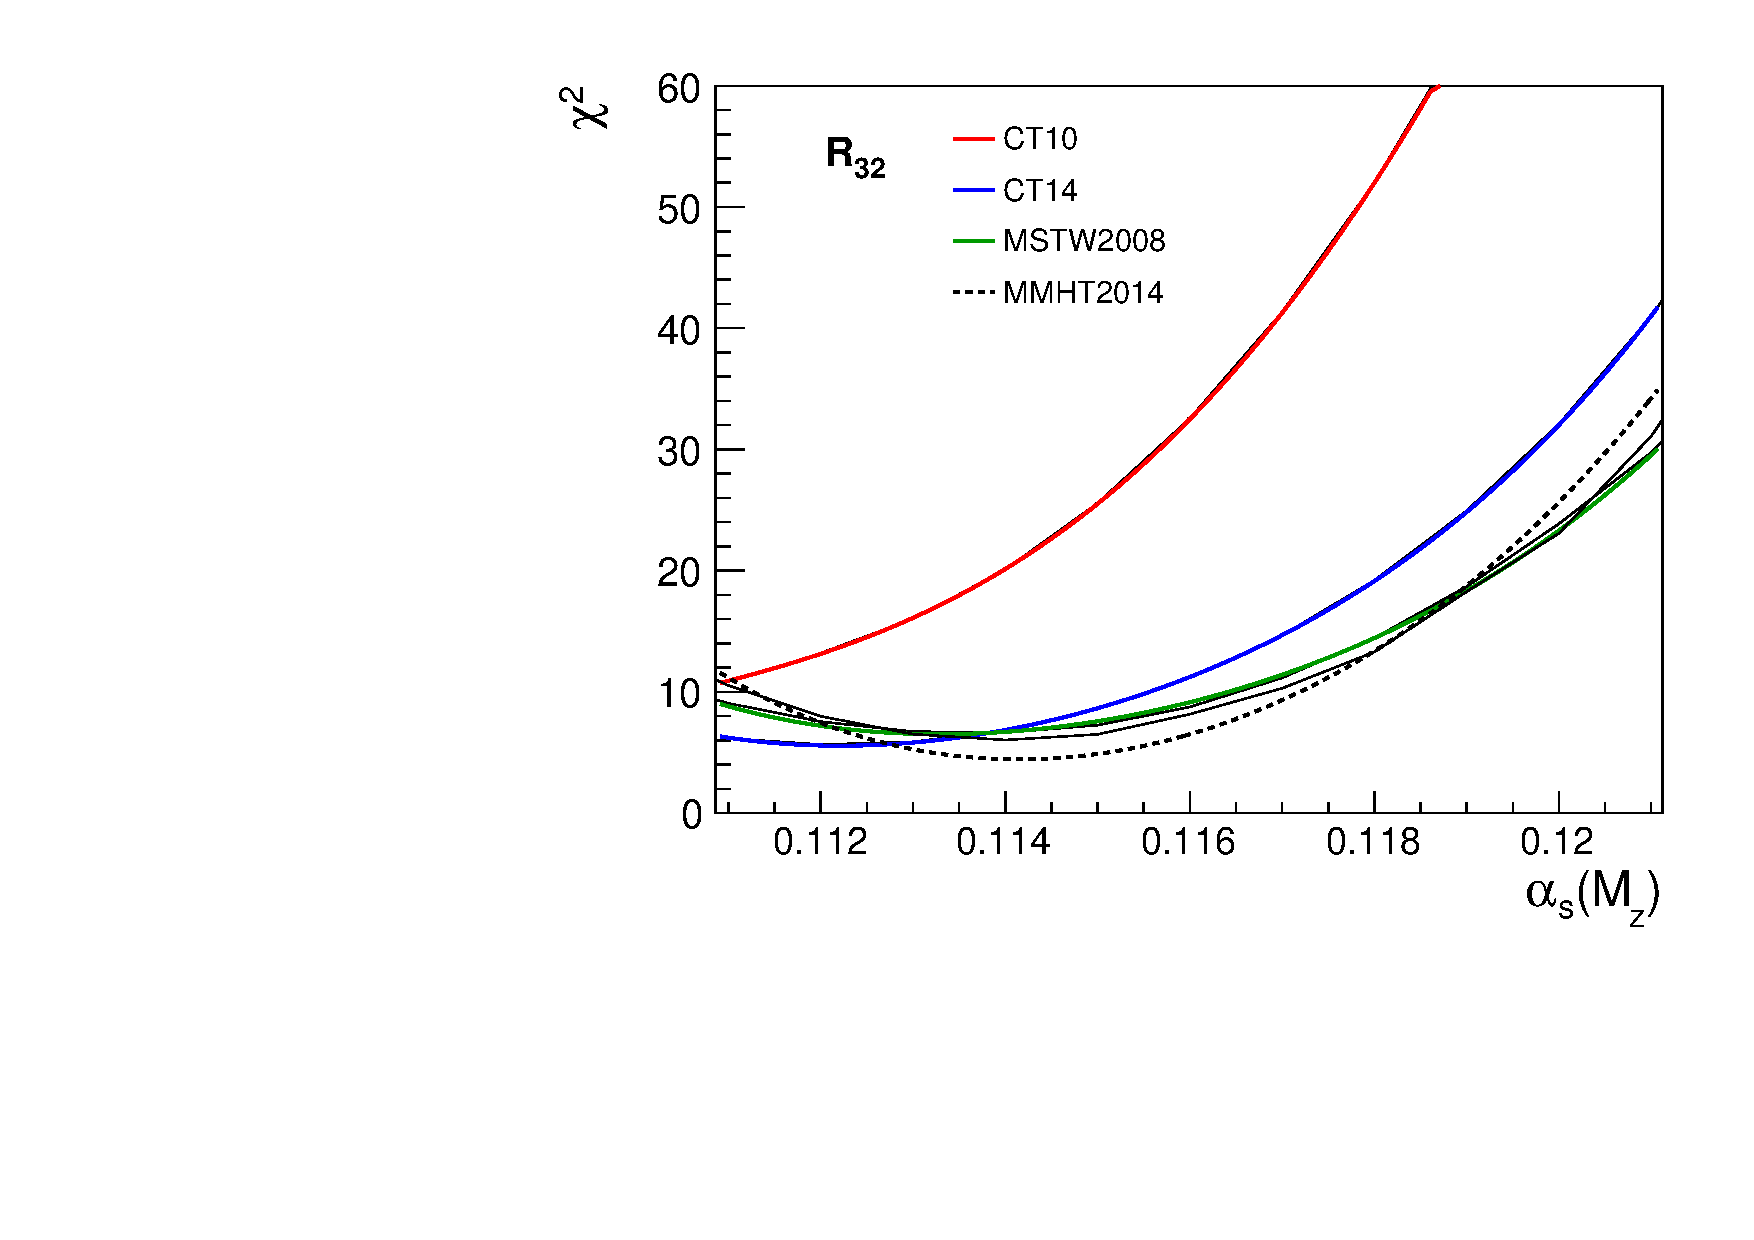
\includegraphics[width=0.5\textwidth]{Plots_HT_2_150/Fits/OutputPlot_r32_100.pdf}\\
%\caption{Variation of Pdf sets.}
%\label{fig:pdf_variation}
%\end{center}
%\end{figure}
%
%\begin{figure}[!htbp]
%\begin{center}
%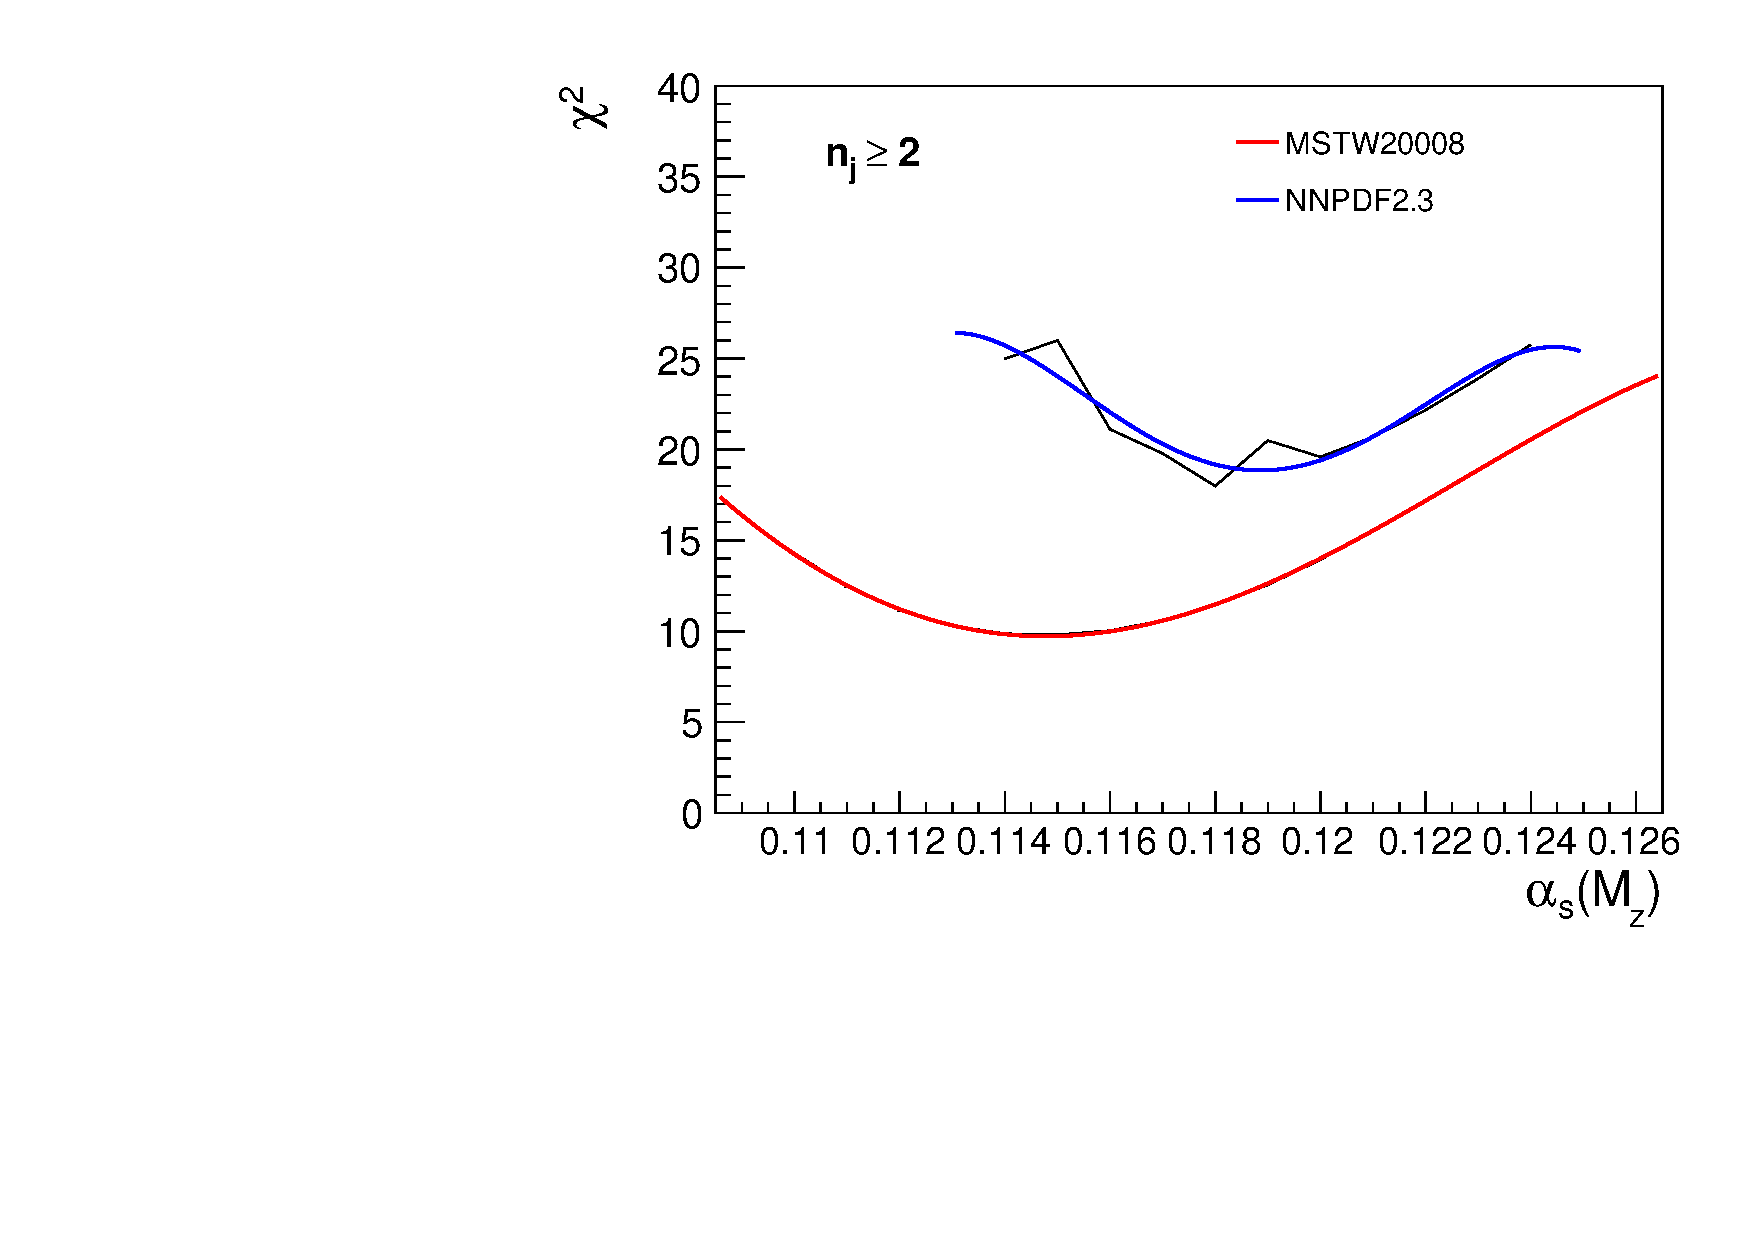
\includegraphics[width=0.5\textwidth]{Plots_HT_2_150/Fits/OutputPlot_2j_100_nn.pdf}%
%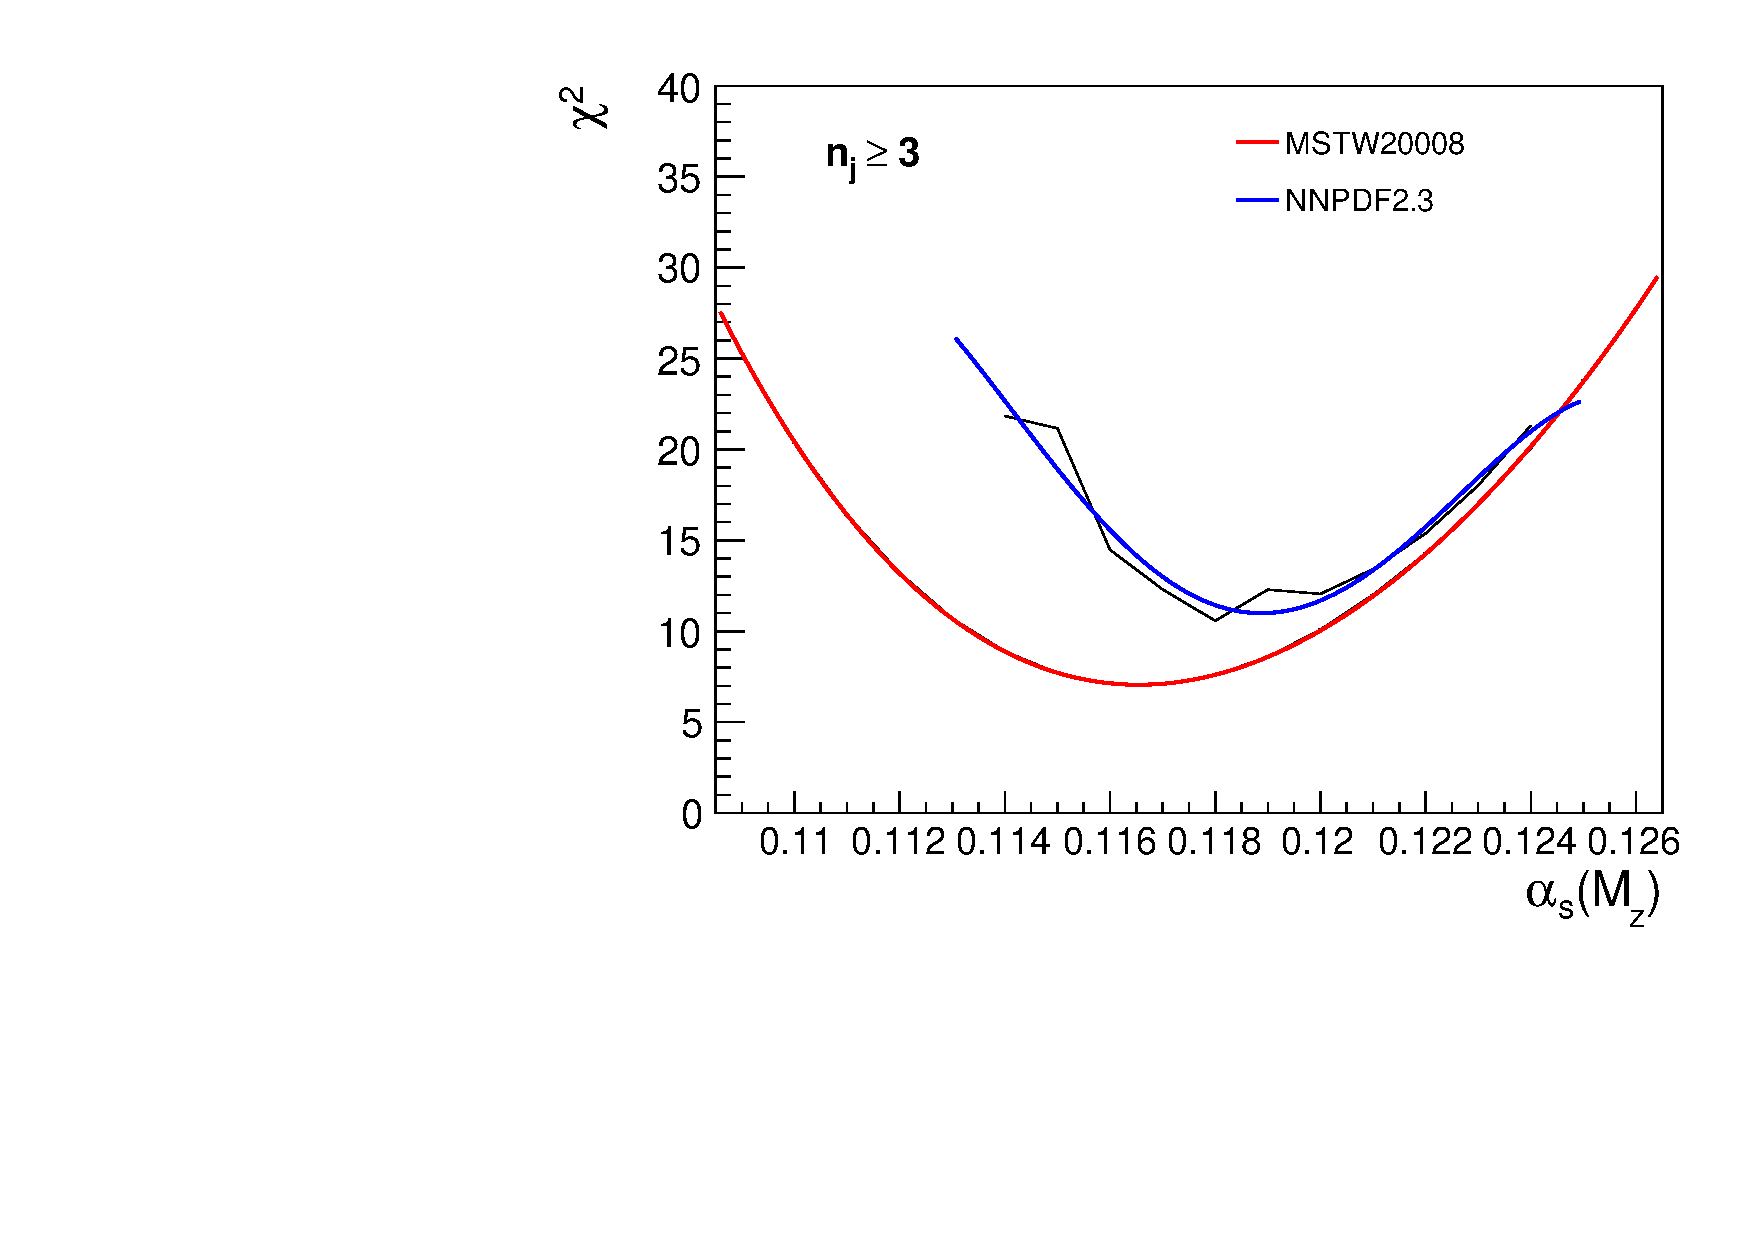
\includegraphics[width=0.5\textwidth]{Plots_HT_2_150/Fits/OutputPlot_3j_100_nn.pdf}\\
%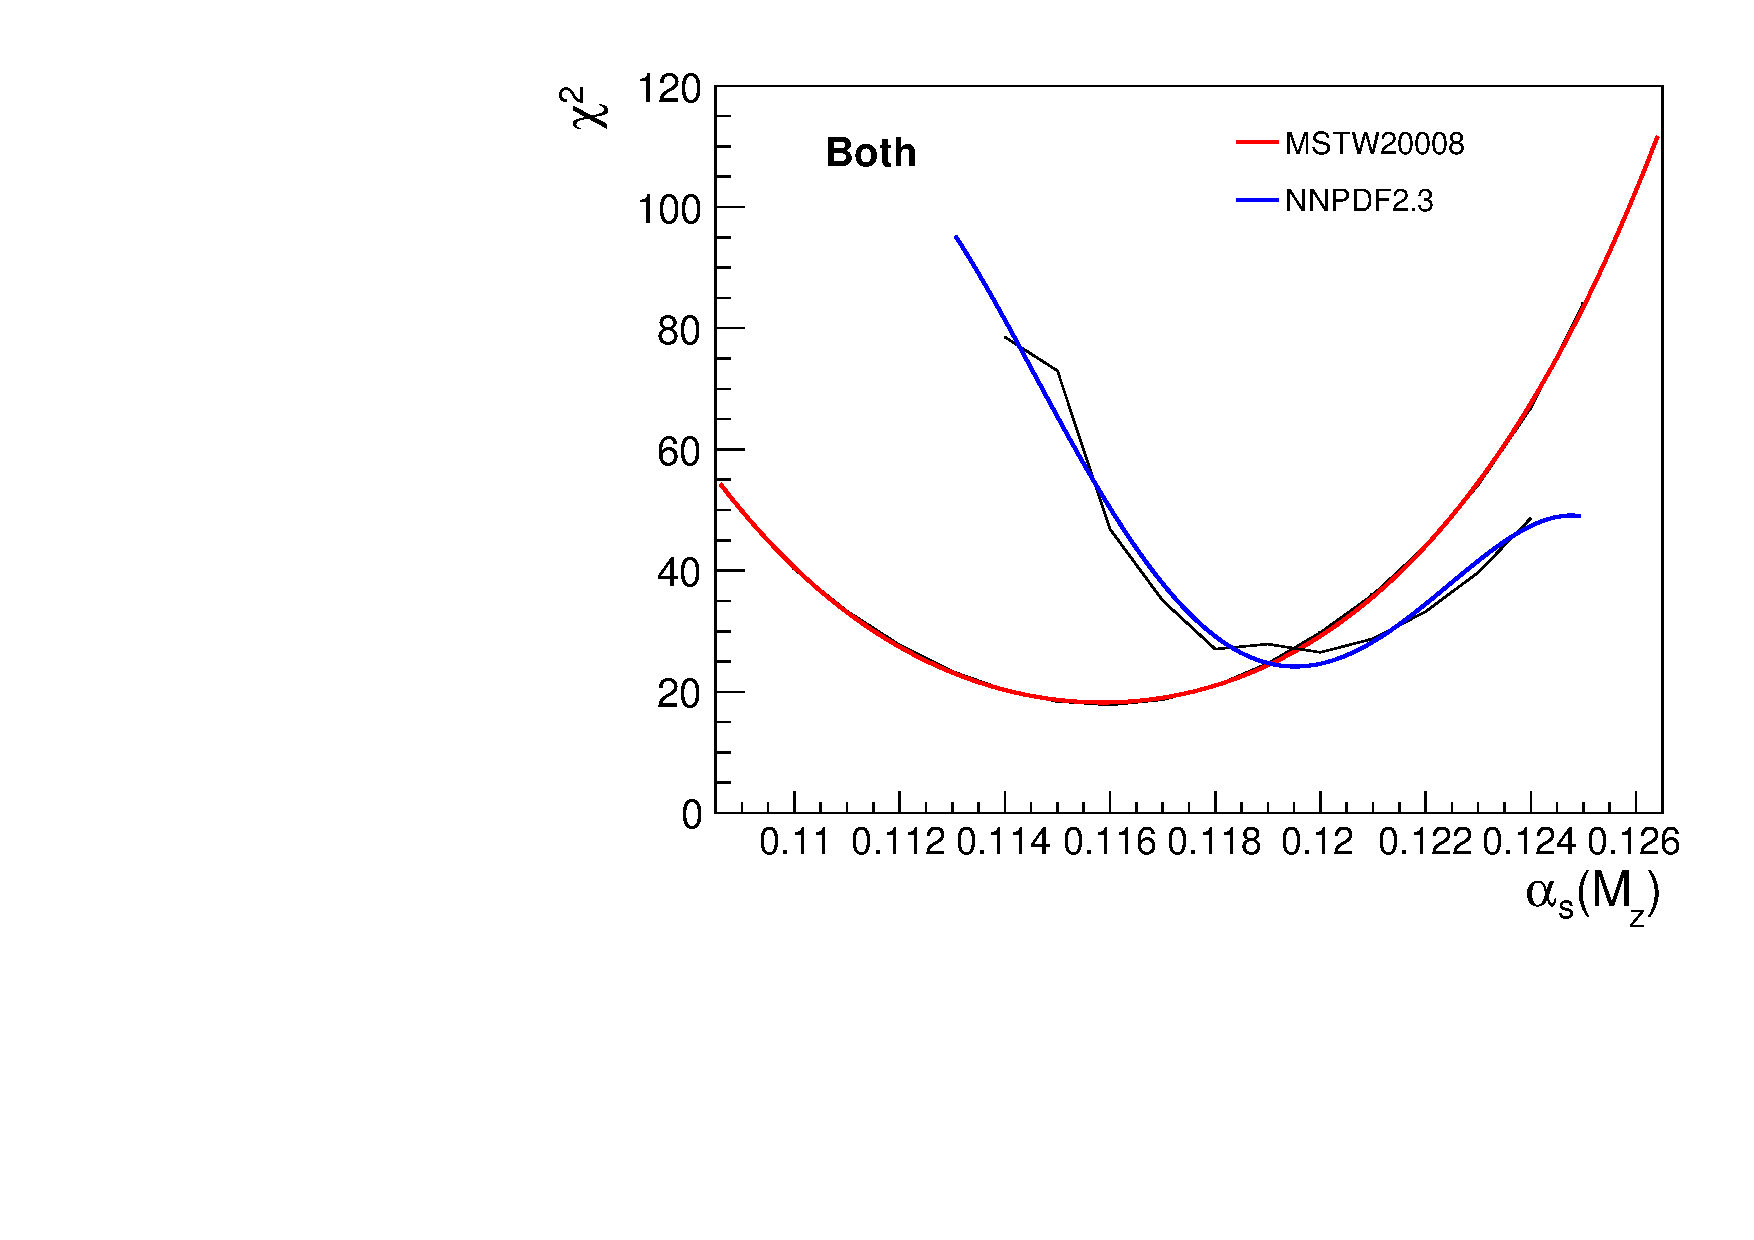
\includegraphics[width=0.5\textwidth]{Plots_HT_2_150/Fits/OutputPlot_nj_100_nn.pdf}%
%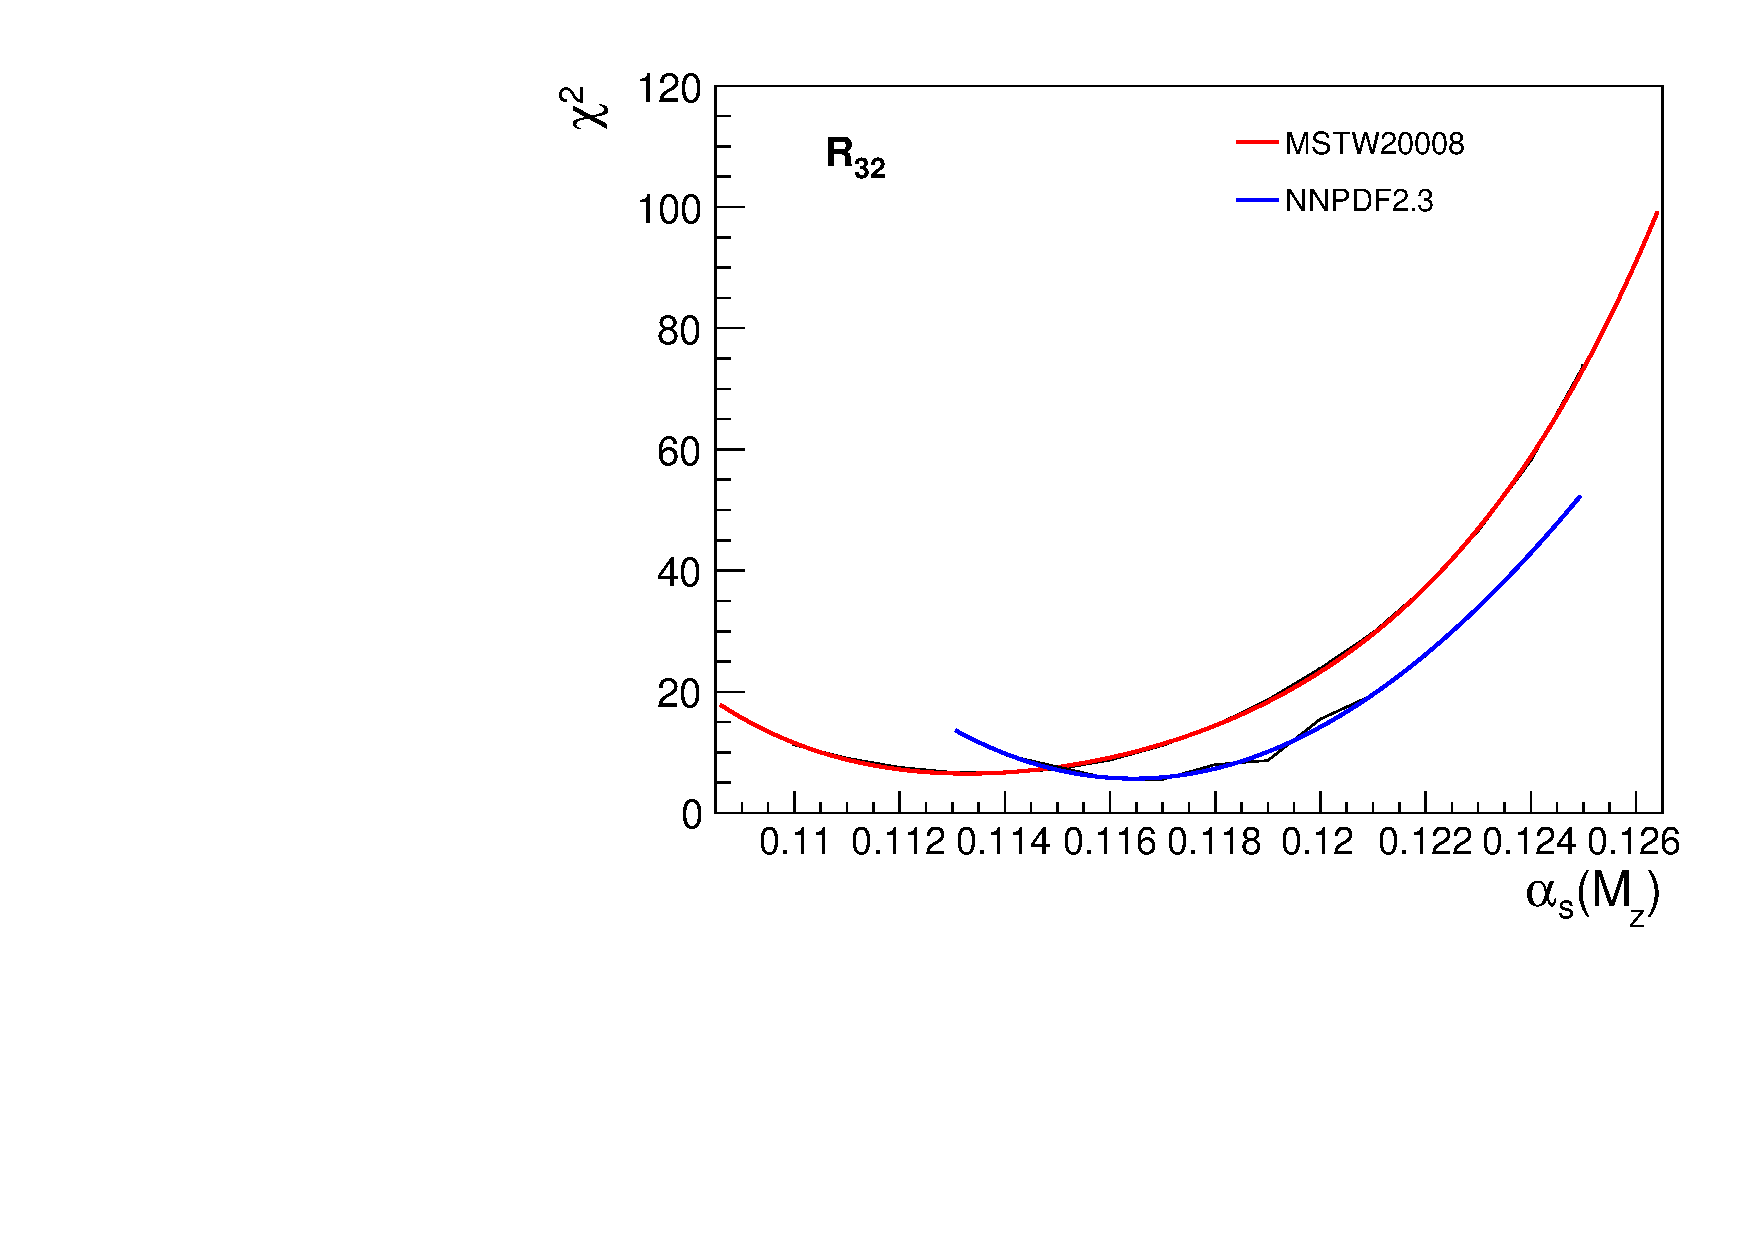
\includegraphics[width=0.5\textwidth]{Plots_HT_2_150/Fits/OutputPlot_r32_100_nn.pdf}\\
%\caption{Effect of randomized NNPDF samples.}
%\label{fig:NNPDF}
%\end{center}
%\end{figure}
\end{comment}
